% Purpose: an example .tex file for the thesis.

\documentclass[11pt,leqno]{report}

\usepackage{ur_thesis}
\usepackage{times}
\usepackage{hyperref}
\usepackage{amsmath}
\usepackage{amsfonts}
\usepackage{graphicx}
\usepackage{tabularx}
\usepackage{listings}
\usepackage[dvipsnames]{xcolor}
\usepackage[font=small]{caption}
\usepackage[nohyperlinks]{acronym}
\usepackage[utf8x]{inputenc}
\definecolor{darkblue}{rgb}{0, 0, 0.5}
\hypersetup{colorlinks=true,citecolor=darkblue, linkcolor=darkblue, urlcolor=darkblue}

\DeclareMathOperator*{\argmin}{argmin}
\DeclareMathOperator*{\argmax}{argmax}
\newcommand{\arr}[0]{\texorpdfstring{$\Rightarrow$}{=>}}
  
% citation style can be whatever is "accepted in your field"
\usepackage[numbers]{natbib}
%\usepackage{natbib}

\begin{document}

\definecolor{codegreen}{rgb}{0,0.6,0}
\definecolor{codegray}{rgb}{0.5,0.5,0.5}
\definecolor{codepurple}{rgb}{0.58,0,0.82}
\definecolor{backcolour}{rgb}{0.95,0.95,0.92}
\lstdefinestyle{mystyle}{
  backgroundcolor=\color{backcolour},   commentstyle=\color{codegreen},
  keywordstyle=\color{magenta},
  numberstyle=\tiny\color{codegray},
  stringstyle=\color{codepurple},
  basicstyle=\ttfamily\footnotesize,
  breakatwhitespace=false,         
  breaklines=true,                 
  captionpos=b,                    
  keepspaces=true,                 
  numbers=left,                    
  numbersep=5pt,                  
  showspaces=false,                
  showstringspaces=false,
  showtabs=false,                  
  tabsize=4
}
\lstset{style=mystyle}

\newcommand{\IE}{\mathbb{E}}
\sloppy
\title{Creating and exploiting metadata for video content recommendation}
\author{Guillaume SANCHEZ}
\thesissupervisor{Frédéric BOUCHARA, Ricard MARXER, Vincente GUIS}
\thesisdepartment{Laboratoire Informatique et Systèmes}
\maketitle

%%%dedication page
\thispagestyle{empty}
%\thispagestyle{plain}
\newenvironment{dedication}
{\cleardoublepage \thispagestyle{empty} \vspace*{\stretch{1}}
  \begin{center} \em}
  {\end{center} \vspace*{\stretch{3}} }
\begin{dedication}

  %% To ... 

\end{dedication}

%%% CV page
%\begin{curriculumvitae}\end{curriculumvitae}

%\begin{acknowledgments}
%  Thanks to collaborators and supporters.
%\end{acknowledgments}

\begin{abstract}

  A brief summary.
  
\end{abstract}



\begin{contributors}

This work was supervised by a dissertation committee consisting of Professors
X, Y, and Z. 
This material is based upon work supported by the National Science Foundation Award
XXXXXXX.  Any opinions, findings, and conclusions or recommendations
expressed in this material are those of the author and do not necessarily
reflect the views of above named organization.

\end{contributors}


\tableofcontents
%\listoftables
%\listoffigures

%\include{facerec}

\chapter{TODO}

The code is available at \url{https://github.com/Vermeille/thesis-code}.

Plan d'action :

Hexa:
\begin{itemize}
    \item Proposer un call à Frank/PA pour faire une lecture rapide et récupérer des infos complémentaires

\end{itemize}

Reco Actions
\begin{enumerate}
    \item DONE: resultat
    \item DONE: ablation: sans transfert
\end{enumerate}

Face rec
\begin{enumerate}
    \item arcface verif -> classifiers \url{https://github.com/TreB1eN/InsightFace_Pytorch}
    
    \item Calibration: avant / après, distribution
\end{enumerate}

Expiration VQ
\begin{enumerate}
    \item DONE: histogram utilisation (age, entropy)
    \item DONE: histogram utilisation sans aging (age, entropy)
    \item DONE: Usage over testset
    \item DONE: regarder xp robust vqvae (ppl vs iter (train / test), test MSE vs codebook size)
    \item Classifier from features
\end{enumerate}

VQFace
\begin{enumerate}
    \item résultat négatif : Images dégueu VAE
\end{enumerate}

CondGAN Facegen ?

Recommender:
\begin{itemize}
    \item Algorithms
    \item figures
\end{itemize}

Tch:
\begin{itemize}
    \item Examples
\end{itemize}

Threshol softmax?
\chapter{Hexaglobe}

%CF ANRT

%\url{https://docs.google.com/document/d/1P65-ilrIhAxT9u5X-E_sTAplCMeGbK9IrOjzs21DI1k/edit}

\section{Activities}

Hexaglobe provides all types of companies in the modern media landscape with technologies and professional services covering the entire process from video ingest to delivery.

Customers are numerous and diverse, from TV channels to radios and \ac{VOD} producers. Hexaglobe takes care of the whole video life cycle: uploading, storage, metadata extraction and management, encoding, referencing, search, and serving.

\section{Problems and motivations}

While classical software engineering is the right tool for encoding, managing, and serving the videos, it almost forces to consider them as impenetrable data blobs. Classical software engineering is very limited to the understanding and semantics that can be extracted from those data.

This is unfortunate. Being able to access the semantics of the videos would help improve the user experience in many ways \citep{contentretrieval}: it would make search more accurate, would allow for fine grain classification or help with recommendations. It would also be useful for the customers that would have more accurate insights into the type of videos that get more views, and would help data analytics with more intelligence. This is especially true for collaborative platforms, akin to YouTube, where the videos are uploaded by non professional people and the user given metadata cannot be relied on.

Very recent development have seen models such as \ac{CLIP} \citep{openaiclip} able to query images from natural languages, confirming the feasibility of the task.

The customer I have been affected to has a massive database of 9M+ user uploaded videos since 2006. That data has very little annotations and metadata, and it is fundamental that those videos can get recommended in a more impactful way, get more accurate categorization and more precise search. All in all, what is needed is to ease browsing and exploit that massive data and make sure nothing high value lies dormant or drowns in this data ocean.

It would also be interesting to modernize the older content with quality enhancement and super resolution techniques, a thing I kept in mind while learning about generative models. This, however, is far beyond the scope of this thesis.

\section{Data}

Throughout the thesis, three datasets have been created and are continuing to be developed as an ongoing process. Those datasets need to be refined, completed, and changed in order to fit the ever growing industrial needs. They are used for training and evaluating models before deployment.

Due to the confidential nature of the datasets, the nature of the data and example samples cannot be revealed.

\subsection{HActions}
\label{sec:hactions}

This first dataset has been manually labeled on my own. It contains pictures of natural images of people going on about what are supposed to be the 12 most popular activities on the website's videos, labeled A to M, plus an extra class that represents any other activity and another one for title screens / text screens showing no humans. The distribution of data samples is shown in Figure \ref{fig:xactions}.

In many activity recognition tasks, the environment can be extremely informative. For instance, karting, canyoning, sailing, driving, climbing, all take place in different environments and there activity clues scattered all over the picture. However, our situation, those activities are decided by body position rather than environment. In some sense, sleeping, singing, dining, watching TV or playing games all take place in a domestic environment and a classifier would have very little clues in the environment to sort them out. Special care would be needed to make sure the classifier do not overfit on spurious background elements for instance.

Since training and inference on full videos would require a lot of compute, we instead assume that still pictures taken from the videos contain enough information for the classification task. 300 evenly spaced frames are extracted throughout videos that lasts more than one minute. That way the computation budget remains fixed and controlled. For comparison sake, if we were to use all the video frames with a temporality aware model, 300 frames would represent a video of 10s only. Even if a video aware model performed much better, the associated costs would be too high, and reducing the frame rate in training and inference would need another pass of video transcoding, which already is expensive.

Instead of randomly splitting the pictures among train / validation / test sets, we randomly split the \emph{videos} in those sets. Not doing this would create validation and test sets containing examples very similar to the ones in the train sets as nearby frames look similar. We aim to have a model that generalizes to videos outside the training set, not frames of a closed set of videos, thus the validation/test sets must contain frames of unseen videos.

\begin{figure}
    \centering
    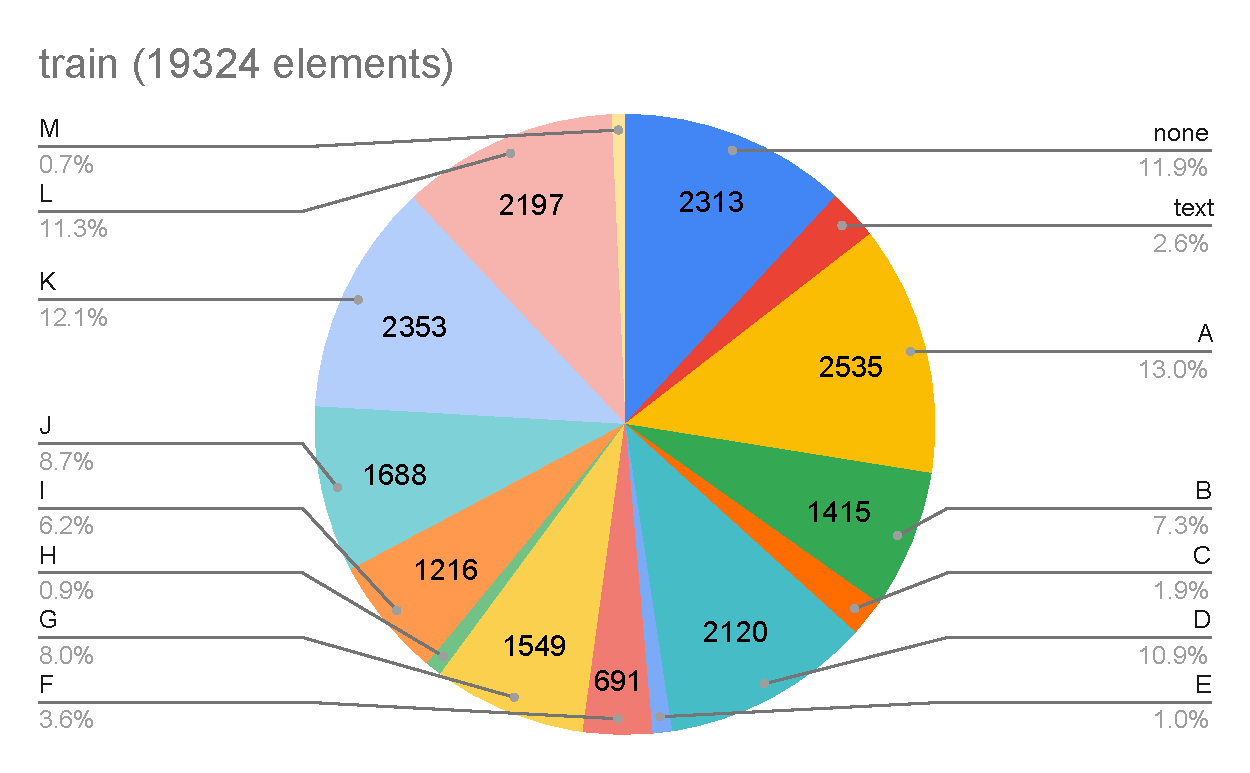
\includegraphics[width=0.45\columnwidth]{20-files/train.pdf}
    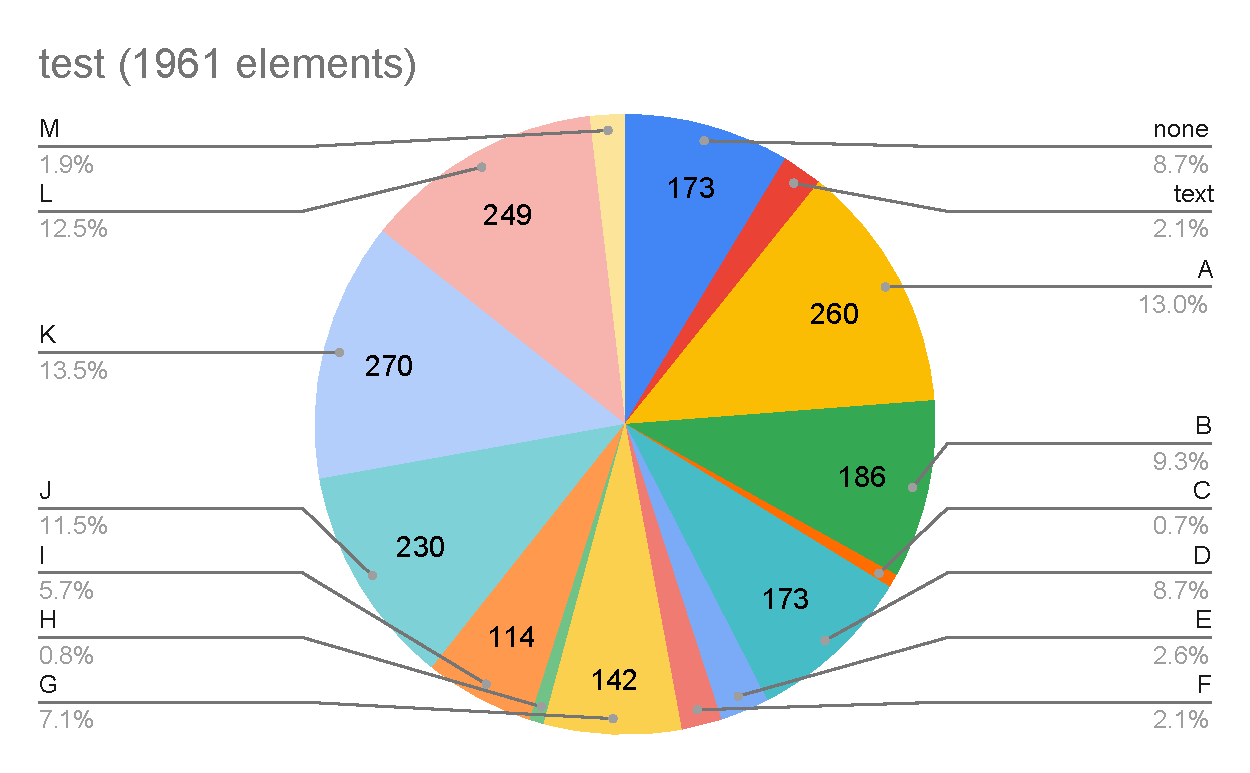
\includegraphics[width=0.45\columnwidth]{20-files/test.pdf}
    \caption{Distribution of samples per classes in HActions.}
    \label{fig:xactions}
\end{figure}

\begin{figure}
    \centering
    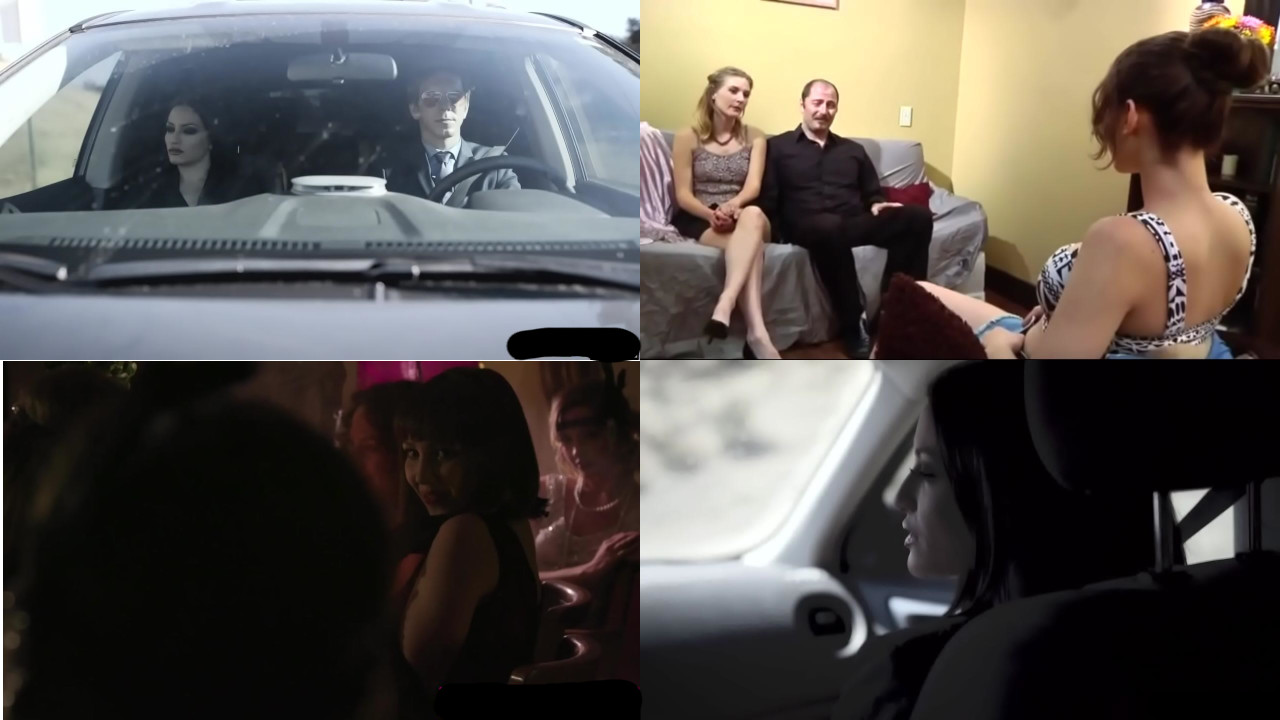
\includegraphics[width=0.7\columnwidth]{20-files/actions.jpg}
    \caption{A few samples from HActions, with class label "none"}
    \label{fig:xactionsamples}
\end{figure}


\subsection{HFaces}

Automatic face recognition would bring very valuable metadata to our content. In our business, identifying celebrities in our domain is one of the core feature that the website's visitors would find valuable.

The dataset contains 8938 identities, but is growing every day as we wish to recognize more people. The distribution of the number of pictures per identities is shown in Figure \ref{fig:xfaces-num}. The dataset has been built with balance in mind. After collecting few very famous identities with web scraping, the labelers have been tasked to manually collect 100 pictures per identity when possible.

Our face dataset is divided into two data sources: faces coming from promotional pictures and coming from videos. Faces coming from pictures are easier to collect but are prone to domain mismatch with videos as they are cleaner: the faces are usually not occluded, there is no motion blur, lighting is good and people tend to smile. In videos, none of this might hold true. We collected many pictures from photos and a smaller bunch from videos in order to evaluate and eventually mitigate the domain mismatch between both.

\begin{figure}
    \centering
    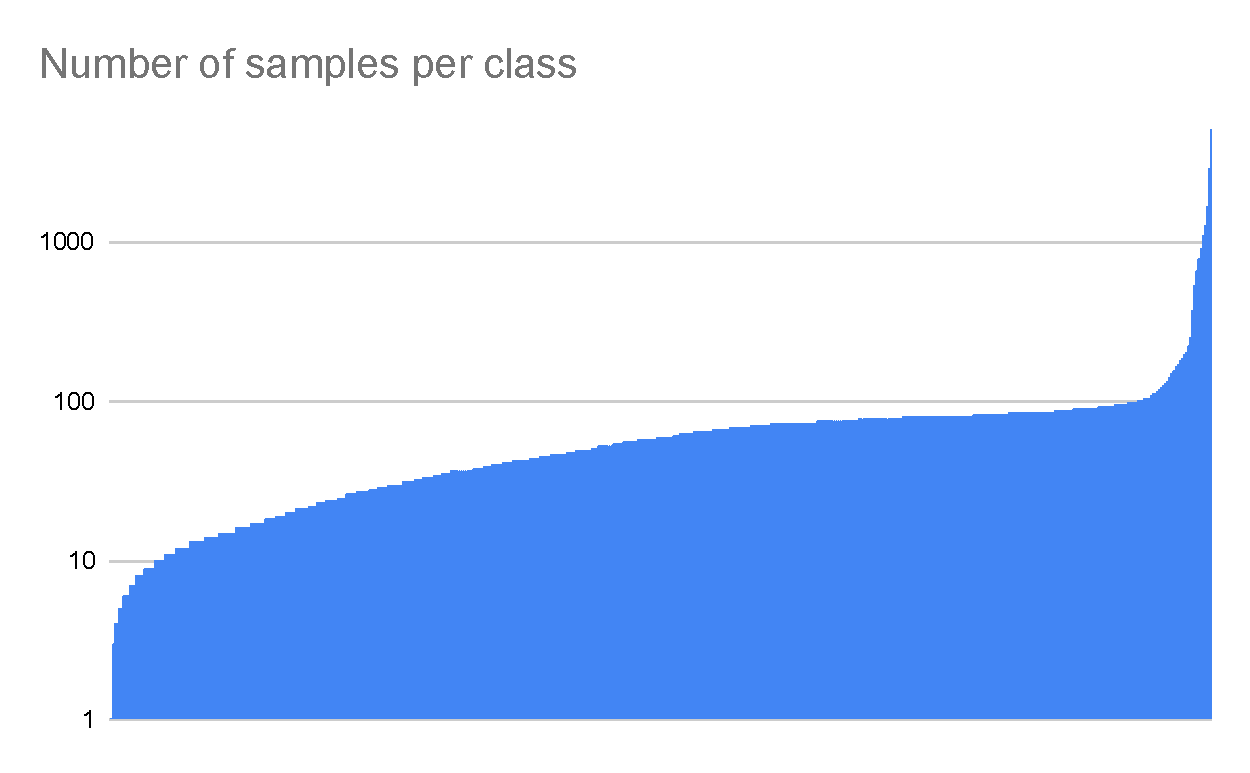
\includegraphics[width=0.7\columnwidth]{20-files/xfaces-num.pdf}
    \caption{Number of examples per identities in the photos subset of HFaces (sorted). Most identities have between 10 and 100 samples.}
    \label{fig:xfaces-num}
\end{figure}

\begin{figure}
    \centering
    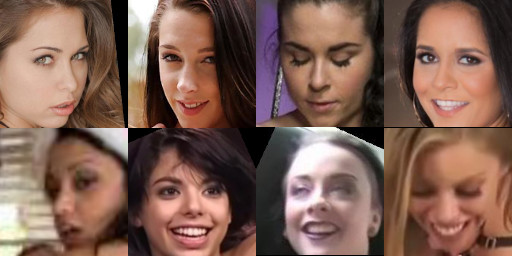
\includegraphics[scale=1.5]{20-files/xfaces-samples.jpg}
    \caption{Samples from HFaces. Top row: extracted from pictures. Bottom row: extracted from videos.}
    \label{fig:xfaces-samples}
\end{figure}

The dataset has been complemented with MS1Mv2 \citep{celeb1m} to provide the so-called "distractors", developped in section \ref{sec:facerec}.

\subsection{HHistory}

\begin{figure}
    \centering
    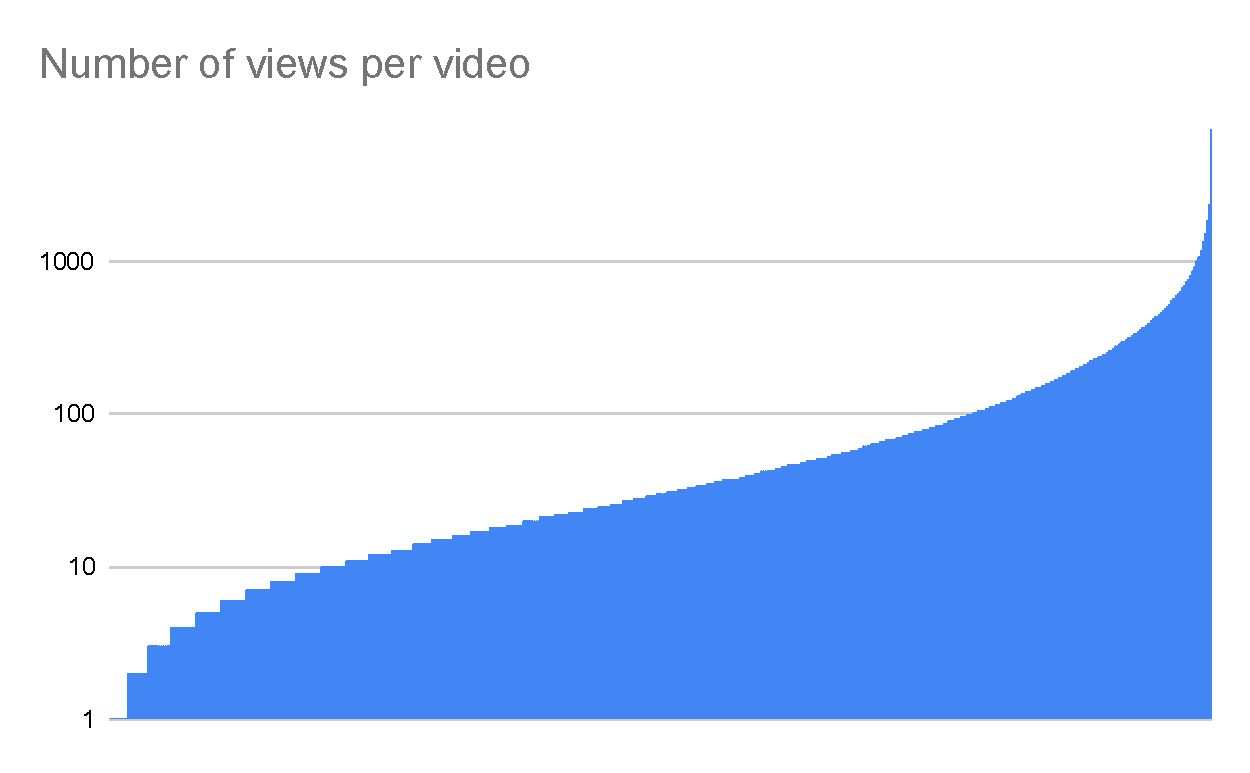
\includegraphics[width=\columnwidth]{20-files/video_views.pdf}
    \caption{Number of views per videos (sorted). Each video is a thin vertical bar.}
    \label{fig:my_label}
\end{figure}

Finally, there is a dataset of premium users' browsing history. This dataset is here to provide historical data for building a recommender system, analyze trends, study semantic proximity of items, etc. This could be useful in various way : videos frequently watched together can serve as contrastive / metric learning dataset to learn about visual features that makes them similar, can learn about tag proximity as well, etc. This dataset can be of many uses and the only metric really lacking is the lenght of watch time per video in order to assess the interest of the user.

Premium content is only a subset of the whole content. The dataset has 135,984 users (content uploader), 3,673 channels and 139,711 videos. It contains various user information, many being optional:

\begin{enumerate}
    \item user ID
    \item username
    \item country / region
    \item gender
    \item liked videos (and the like action timestamp)
    \item disliked videos (and the dislike action timestamp)
    \item favorited videos
    \item watched videos (and their watch timestamp)
    \item channels subscriptions
\end{enumerate}

Similarly, metadata about videos are:

\begin{enumerate}
    \item video ID
    \item main category
    \item the uploader's channel ID
    \item people appearing in the video (from the face recognition model or the previous system)
    \item title (possibly in multiple languages)
    \item various free form tags chosen by the uploader
    \item video encoding quality
    \item upload timestamp
\end{enumerate}

Finally, each channel has popularity scores per category and region.

\subsection{A note about open datasets}

The reader used to academic benchmark and comparisons might object and argue that there are open datasets covering the kind of problems dealt with here. Indeed none of those tasks are new. That being said, each use case is unique in its own way and models fitted on those datasets can't be straightly used for the industrial needs.

HActivity can be thought to be similar to YouTube-8M \citep{youtube8m}. The actions in HActivity have zero overlap with YouTube-8M, so it definitely cannot be used there. Also, as discussed before, the actions in YouTube-8M are often highly informed by environmental clues and much less by body pose.

HFaces resembles CelebA \citep{celeba} / MS1M \citep{celeb1m}. Both those datasets have a vast majority of neutral faces facing the camera. In our situation, the face are quite often non neutral and highly expressive, like faces during sports could be, are quite often not facing the camera, suffer from motion blur, occlusions, and MPEG encoding artifacts.

HHistory is harder to relate to MovieLens \citep{movielens} and Netflix \citep{netflix}. Those datasets are centered around ratings. While HHistory has some, they are both binary and scarce, and most of the training supervision has to be extracted from watch history instead.

\section{Machines}

To work, Hexaglobe provides me three machines, hosted by our Cloud computing provider.

\begin{enumerate}
    \item gpu1 has 2 NVIDIA GTX 1080 Ti and is used mainly for production and inference.
    \item gpu2 has 4 NVIDIA RTX 2080 and is used for my main experiments. It allows me to iterate quickly during development by using large batch sizes.
    \item gpu3 has 2 NVIDIA RTX 2080. This machine is used for runs that I don't mind waiting or for side experiments.
\end{enumerate}

The university also provided several clusters that I could use when working on public datasets.
\chapter{Machine Learning}

As an introductory material, this chapter introduces what Machine Learning is and how it works. This chapter will illustrate the notions through the lens of activity recognition in images. However, the foundations laid out here are not limited to this use case and are indeed more general. The explanations will alternate between the specific use cases, to ease the intuitive understanding, and the more abstract concepts in order to make the generality of the techniques clear.

At the end of this chapter we will illustrate the foundations laid out here with a practical example. This will allow us to introduce the basics of model training, evaluation, data augmentation, and fine-tuning a pretrained model.

\section{What is Machine Learning}

\subsubsection{ML as functions}

Let $\mathcal{X}$ be the set of  images we are interested in, and $\mathcal{Y}$ be the set of activities. In order to solve the problem of activity recognition, we wish to find a function $f:\mathcal{X}\mapsto\mathcal{Y}$ that maps an image from $\mathcal{X}$ to its correct activity. 

While researchers have tried to write themselves algorithms that deciphers natural images, applications such as "search images by text" in Google Photos, image colorization, natural image generation or captioning remained out of reach. Indeed, researchers found more success writing algorithms that \emph{search} for $f$ rather than finding $f$ themselves. Image understanding is now dominated by \emph{machine learning} approaches, that is, algorithms finding $f$ from examples.

In fact, $\mathcal{X}$ does not have to be images, and $\mathcal{Y}$ class labels. As long as there is a relationship between $\mathcal{X}$ and $\mathcal{Y}$, the former can be considered a random variable and the later a dependent variable. Machine Learning is about getting better at a task (with respect to a chosen metric) based on experience (or "examples", or "training samples").

\subsubsection{Parameters and hyperparameters}

In machine learning, we distinguish two kinds of values: parameters and hyper-parameters.

The values or decisions that are searched during learning for representing $f$ are the \emph{parameters}. For neural networks (defined later) they could be the individual neurons' synapses values, or \emph{weights}.

Sometimes, there are configurations for those algorithms that cannot be learnt during training, like the number of neurons or layers, the maximum depth of a decision tree, which are the aforementioned \emph{hyperparameters}.

\subsubsection{Train, validation, and test datasets}

Let a dataset $\mathcal{D}_t={(x_0, y_0), ...(x_N, y_N)}$ where the $x_i \in \mathcal{X}$ are the images and the $y_i \in \mathcal{Y}$ are their class labels (most of the time provided by humans), usually an integer between 0 and $|\mathcal{Y}|-1$. Machine Learning (ML) aims to find a function $f$ that, based on the examples provided in $D_t$, can approximate a correct $f$. This is usually called \emph{training or learning a model}.

Unfortunately, those functions found by ML techniques build complex relations hard to interpret by humans, sometimes known to be coarse approximations. Deep Learning solutions, and sometimes classical ML solutions are often considered black box. If we were able to understand it or not use approximations, we would have probably been able to write the function in the first place. It is often not possible to verify that the model solves the task in a meaningful way by checking its inner workings. Checking a ML model usually involves having a second set of annotated data $\mathcal{D}_v$ and checking the performance (accuracy, for instance) on this set of data, called \emph{validation set}. We have to rely on the validation set performance in order to trust that if the model solves them, then it has found an appropriate solution.

Finally, there is another catch. Some algorithms need to be configured with some \emph{hyperparameters} before learning on the training set. However, throughout a project's life, the model and algorithms evolve during development. In order to make sure those hyperparameters and this exact algorithm generalize well and are not just conveniently working for this validation set, there is usually a third set, the \emph{validation set} that is used in place of the test set during both development and hyperparameters selection. The test set $\mathcal{D}_e$ is used as little as possible, only when trying to have a clear evaluation of the performance of the model. The test set, in order to be predictive of the model's final performance, should be representative of the real world data.

Every time the developer or the learning algorithm tunes parameters or hyperparameters, there is a risk that they become tailored to this dataset exactly. This is called overfitting: decreasing generalization and improving the performance on the training set. The test set exists to test whether the learning algorithm overfitted parameters on the training set.

The developer adjusts various hyperparameters (model size, learning rate, etc) in order to maximize the performance on the validation set. In order to make sure that those hyperparameters decisions generalize beyond the test set, we need a third set, the validation set. Unfortunately, as we use more and more the validation set to test various models, there is a risk of overffiting it as well.

Indeed, some datasets are used so commonly by researchers that there is a risk that the models and algorithms tested on those don't generalize as well and are accidentally tuned to those datasets specifically \citep{imagenetgeneralizeimagenet}.


\section{Neural Networks}

\subsection{Neural Networks in computer vision}

While there are many algorithms that are able to learn from examples, computer vision is nowadays largely dominated by neural networks. They gained a lot of traction in 2012 when the ImageNet challenge \citep{imagenet} was won by a large margin with neural networks \citep{alexnet} rather than classical image processing techniques using classical machine learning (kNN, SVM, decision trees, etc \citep{bishop}). The next year, in 2013, all competitors used neural networks. In 2015, they started gaining traction in the industry as well. I can remember, that year, when interning in Google, Sundar Pichai pitching Google Photos and explaining how big resnets \citep{resnet} made it possible, less than a full year after their discovery.

\subsection{Neurons}

\begin{figure}[h]
    \centering
    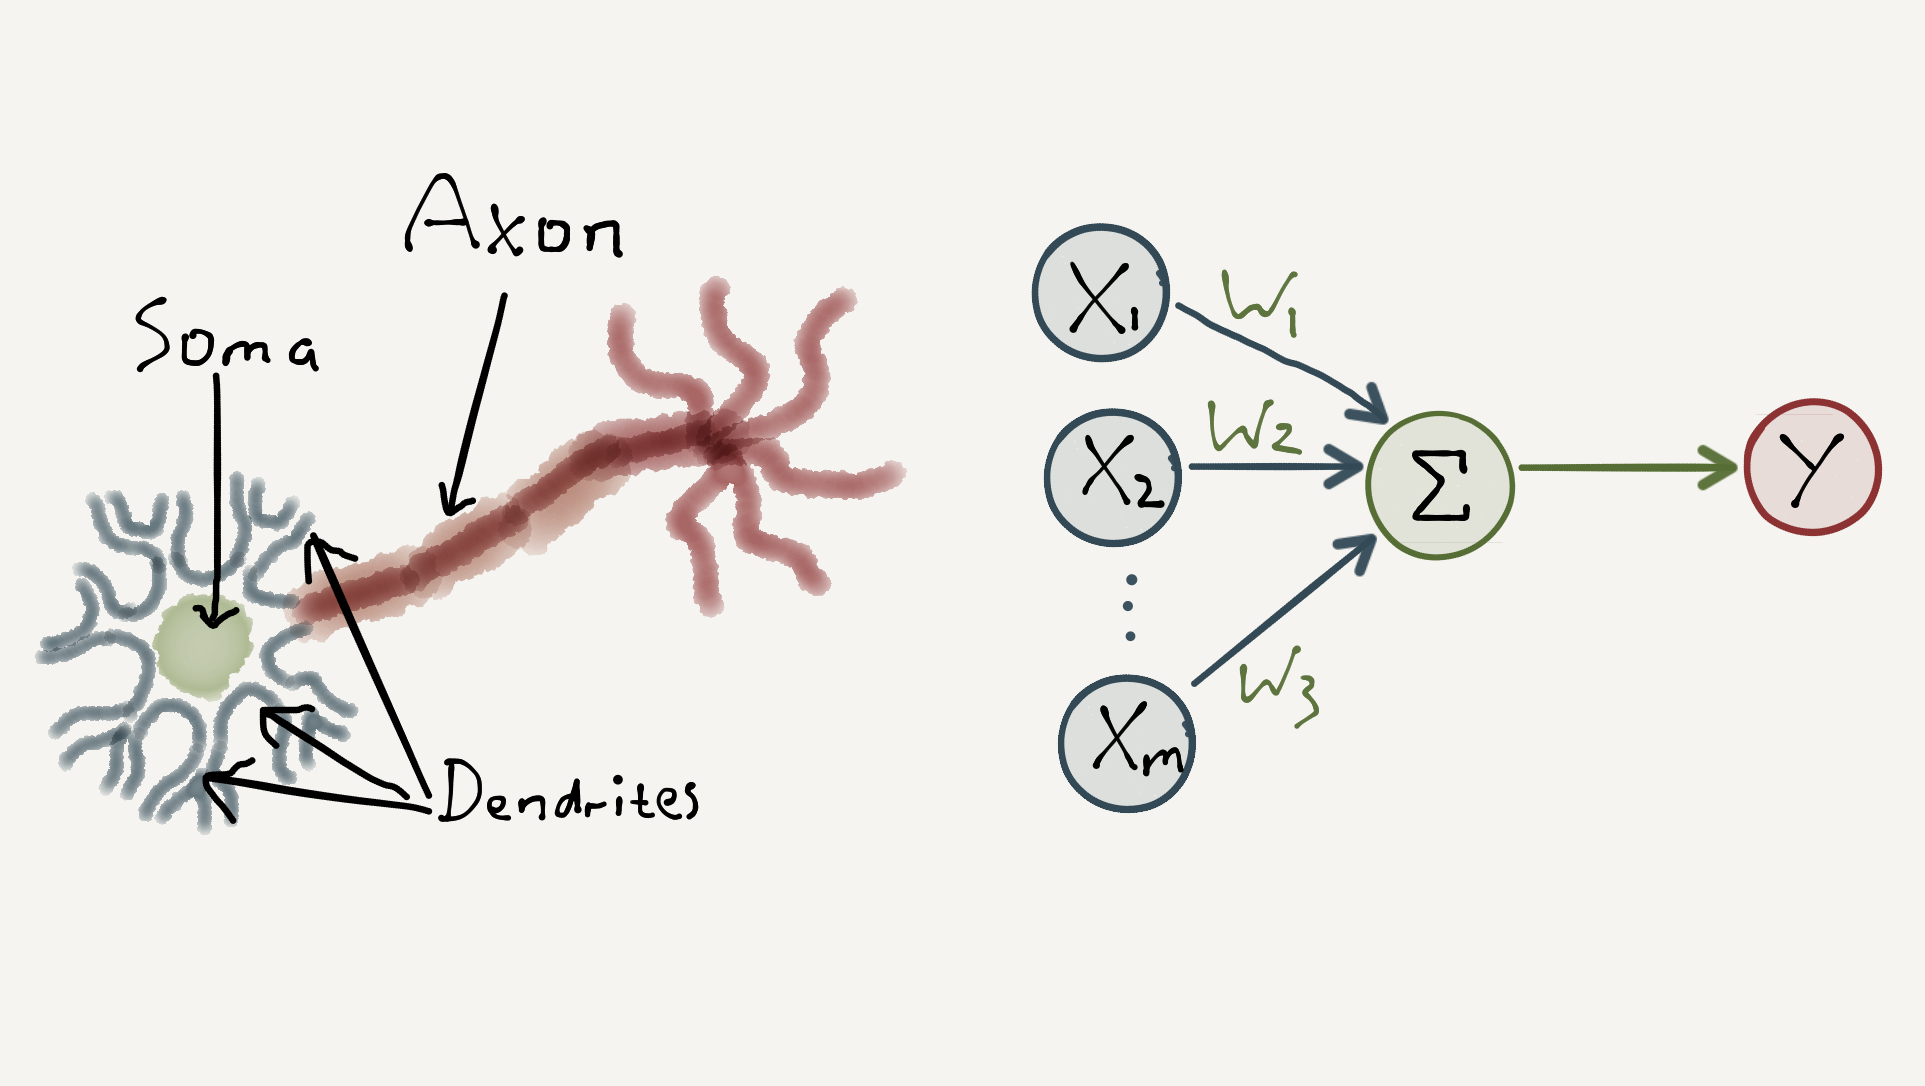
\includegraphics[scale=0.1]{30-activity/neuron.png}
    \caption{A (very simplified) biological neuron and an artificial neuron (Perceptron)}
    \label{fig:neuron}
\end{figure}

Before understanding neural networks, let's focus on a single artificial neuron. Artificial neurons are loosely inspired by biological neurons. They represent a neuron taking some input electrical signals, transmitting those by weaker or stronger dendrites (connections), summed up in the soma, firing through the axon if the total amount is above a certain threshold. Cf Figure \ref{fig:neuron}

In computer science, this is approximated by a linear combination $\textbf{w}$ - a weighted sum - of the input $\textbf{x}$, followed by a threshold $b$ and an activation function $\sigma$. An artificial neuron is then $\sigma(\textbf{w}^T\textbf{x}+b)$, with $\sigma$ being any non-linear function. \emph{Training a neuron is finding the weights $\textbf{w}$, $\textbf{b}$ that works best for solving a given problem}. This is sometimes still called a Perceptron, in reference to the original paper by \citet{perceptron}.

While today we often chose the \emph{Rectified Linear Unit} (ReLU) $\sigma(x)=\max(0, x)$ for its good numerical and computational properties \citep{relu}, researchers initially used a sigmoid, tanh or step function. Developing on activation functions is well beyond the scope of this manuscript, but it is still an active area of research with new propositions, despite none of them outperforming the performance / computational cost tradeoff of ReLUs.

\subsection{From single neurons to neural networks}

Once we have a neuron, there are two ways we can add more to build a \emph{neural network}: either by parallel neurons (the \emph{width}) or by stacking them in successive \emph{layers} (the \emph{depth}). The Universal Approximation Theorem \citep{universalapprox} states that a neural network with 2 layers and enough neurons \cite{mlpbounds} can theoretically approximate any computable function. Unfortunately, possible does not equate practically feasible and we needed decades before turning them into useful algorithms. The deception lies in the "enough" part, which can be intractable for any practical purpose.

Fortunately, it has been shown that width can be traded with depth \cite{widthdepth}, allowing neural networks to work in successive abstractions \citep{deepbelief,deepviz}, thus not needing stellar amount of data and compute. Deepening neural networks was not possible immediately, and required new tools (among which the aforementionned ReLU), explaning why neural nets remained shallow for so long.

\subsection{Training neural networks}

\begin{figure}
    \centering
    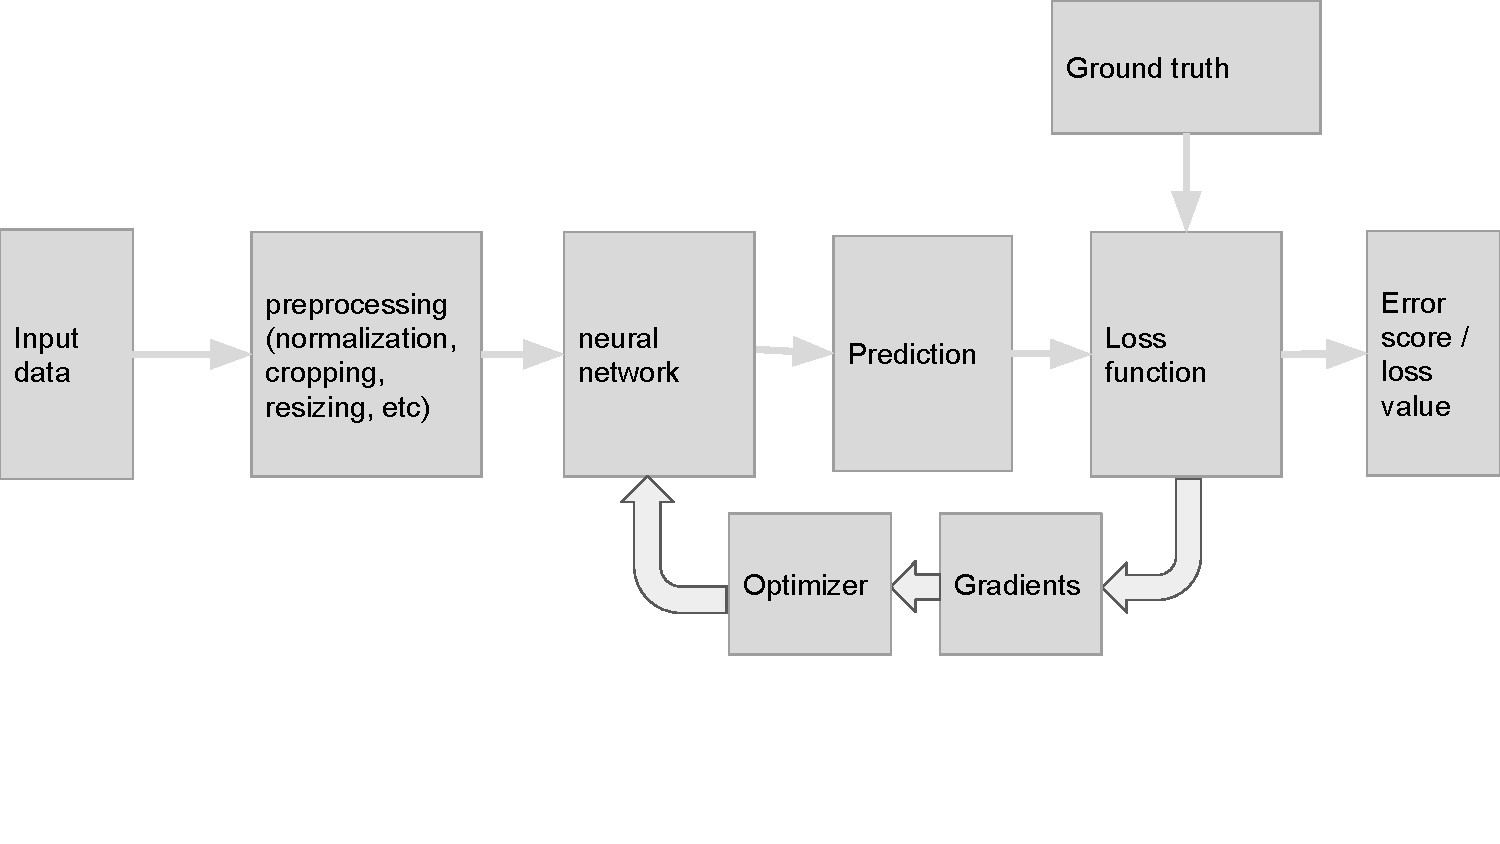
\includegraphics[width=\columnwidth]{30-activity/workflow.pdf}
    \caption{A neural network training loop}
    \label{fig:trainingloop}
\end{figure}

After describing what neural networks \emph{are}, it is necessary to describe how they \emph{work}. Neural networks are stacks of non-linear layers, composed of many tunable weights $\theta$ computing data transforms. How do we train them?

Neural Networks are built from differentiable components, making $f_\theta(\cdot)$, the function they compute, differentiable as well. In the simplest case, the training dataset provides an input $x$ and expected correct answer $y$. We compute $\hat{y}=f(x)$, the maximum likelihood answer given by the network. Then, a differentiable predefined function $\mathcal{L}(\hat{y}, y)$ computes the distance between the generated answer and the expected correct answer. By differentiating this distance wrt to the parameters $\theta$, we get the direction in which to move $\theta$ to reduce the error. $\theta$ is moved a bit (a step of size $\alpha$) in this direction and the iterative process continues, and $f$ learns to provide better and better answers. This process is called \emph{Gradient Descent}. In Deep Learning, however, \emph{Stochastic Gradient Descent} (SGD) is used. The stochasticity comes from the fact that we compute the gradient on a random subset of the dataset (a \emph{batch} or minibatch), each iteration. This helps regularizing the model (thus providing greater generalization), and descending on the full dataset is often not practically doable anyway since they are usually too big to fit in memory along with the gradient information. Each iteration thus fundamentally computes

\begin{equation}
    \theta := \theta - \alpha \nabla_\theta \mathcal{L}(f_\theta(x), y)
\end{equation}

However, as we will later see, this update equation can be made more sophisticated in order to reduce the number of steps needed to converge and / or improve generalization. These approaches are called \emph{optimizers}.

This process is summarized in Figure \ref{fig:trainingloop}.

\subsection{Data Augmentation}
\label{sec:trivialaugment}

Last but not least, neural networks have the capacity to fit and memorize even big datasets. When the networks start to memorize the training set, the model overfits and its generalization abilities decrease. One way to fight against that overfitting is to add more training data, but this is often expensive or hard. Instead, one can create artificial new examples by modifying the training set. For images, this can be flipping the pictures, rotating them, changing the illumination, etc. This also injects domain knowledge into the algorithm about the existing invariances. This is called \emph{data augmentation}. Tremendous progress has been made thanks to augmentation strategies \citep{cutmix,randaugment,mixup}. Examples from AutoAugment from \citet{autoaugment} are shown in Figure \ref{fig:autoaugment}.

\begin{figure}
    \centering
    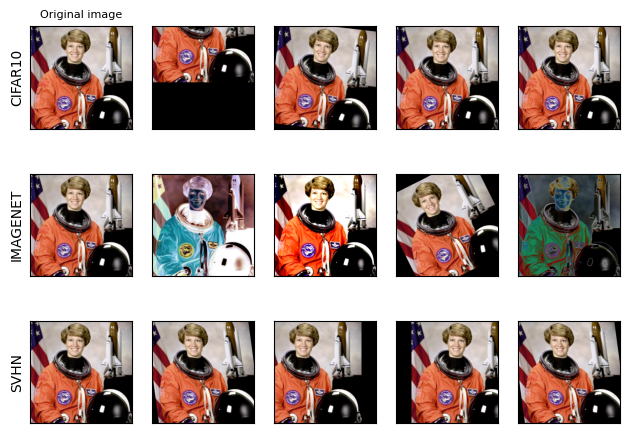
\includegraphics[width=\columnwidth]{70-files/autoaugment.png}
    \caption{Example of data augmentation. The original image is transformed to artificially generate new training examples. In this case, AutoAugment is used ; it combines multiple transformations and its settings depend on the dataset and the task. Figure from torchvision's documentation. Each row shows the set of augment used for those datasets on a sample image.}
    \label{fig:autoaugment}
\end{figure}

In this work, we will mainly use TrivialAugment \cite{trivialaugment}. It is a recent and very simple augmentation algorithm from which we can learn that despite a lot of complicated methods to automatically find augmentation policies (AutoAugment \cite{autoaugment}, RandAugment \cite{randaugment}, ...), yet the simplest method performs comparably or better.

TrivialAugment defines an augmentation as "a function a mapping an image x and a discrete strength parameter m to an augmented image". It uses a collection of predefined classic image transformations (color, contrast, rotation, ...). It randomly selects one of this operation per sample, and randomly sample its strength parameter m.

\subsection{Architecture}

What those layers of neurons compute and how they are arranged define an \emph{architecture} or \emph{topology}.

When two or more Perceptrons layers are stacked, it is called a \ac{MLP}.

However, Perceptrons do not perform well on natural image data. They are too general and somehow too powerful for computer vision: a Perceptron treats each and every input as separate variables, but pixels values are not independant variables. First, they are spatially correlated as the world is compositional, and exhibits many invariances in translation, scale, and orientation.

Perceptrons have to learn to perform the same operations everywhere on the picture, and, in practice they don't. Replacing Perceptrons with convolutions with learnable weights gave birth to \acp{CNN}.

A convolutional layer is a Perceptron in disguise. It is just applied repeatedly and similarly on smalls spatial patches of the input. The size of that input patch is called \emph{kernel size}. We compute many different convolutions on the same input - the \emph{width} of the convolutional layer. Perceptrons compute multiple different linear combinations of the input in the same way -, each resulting spatial map is called a \emph{feature map} or \emph{channel}. Finally, the convolution kernel can jump some inputs, we call this \emph{strided} convolutions, in order to downsample the input resolution.

Convolutions instead of Perceptrons builds into the model what are called \emph{inductive biases}: they perform local operations - addressing compositionality - and performs them the same way everywhere on the picture - addressing translational invariance -. \acp{CNN} got fame in 2012 when they beat their competitors in the ImageNet classification challenge by a large margin and created the deep learning hype we know today \citep{alexnet}.

\begin{figure}
    \centering
    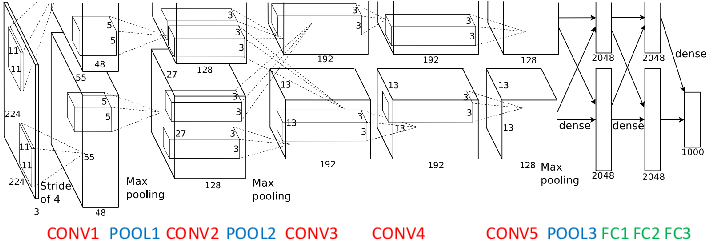
\includegraphics[scale=0.5]{30-activity/AlexNet.png}
    \caption{AlexNet architecture, built from convolutions (CONV), pooling operations (POOL), and linear layers (FC). Figure from \citet{alexnet}}
    \label{fig:alexnet}
\end{figure}

The convnet that made deep learning attractive by winning ImageNet is \textbf{AlexNet} \citep{alexnet} (see Figure \ref{fig:alexnet}). It contains 5 conv layers, 2 max pooling layers, and 3 linear layers (also called Fully Connected layers). Max Pooling are meant to reduce the spatial size in order to reduce both memory and compute consumption, and increase the working region of each convolution. As the image is processed through the convnet, it produces layers of activations, that gets abstracted in neural representations. Deep representations have a low spatial resolution but rich semantics \citep{deepbelief,deepviz}.

\begin{figure}
    \centering
    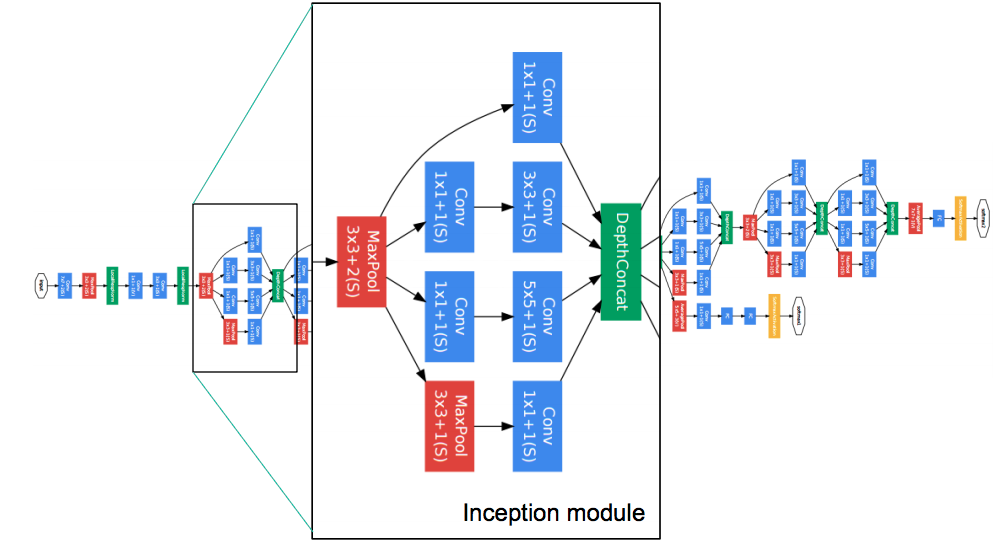
\includegraphics[width=\columnwidth]{30-activity/googlenet.png}
    \caption{GoogLeNet / Inception-v1. It uses complex building blocks, aggregating different design decisions. Figure from \url{https://medium.com/@RaghavPrabhu/cnn-architectures-lenet-alexnet-vgg-googlenet-and-resnet-7c81c017b848}}
    \label{fig:googlenet}
\end{figure}

The design of convnets raises many questions: how many channels? what kernel shape? what stride? Should we pool? It is hard to answer those, so, when designing \textbf{GoogLeNet} / \textbf{Inception} \citep{googlenet} (Cf Figure \ref{fig:googlenet}), the Google team stacked many layers of complex building blocks. Each of those blocks is composed of parallel paths taking different design decisions. At train time, the net can learn to use each of those paths to its best.

\begin{figure}
    \centering
    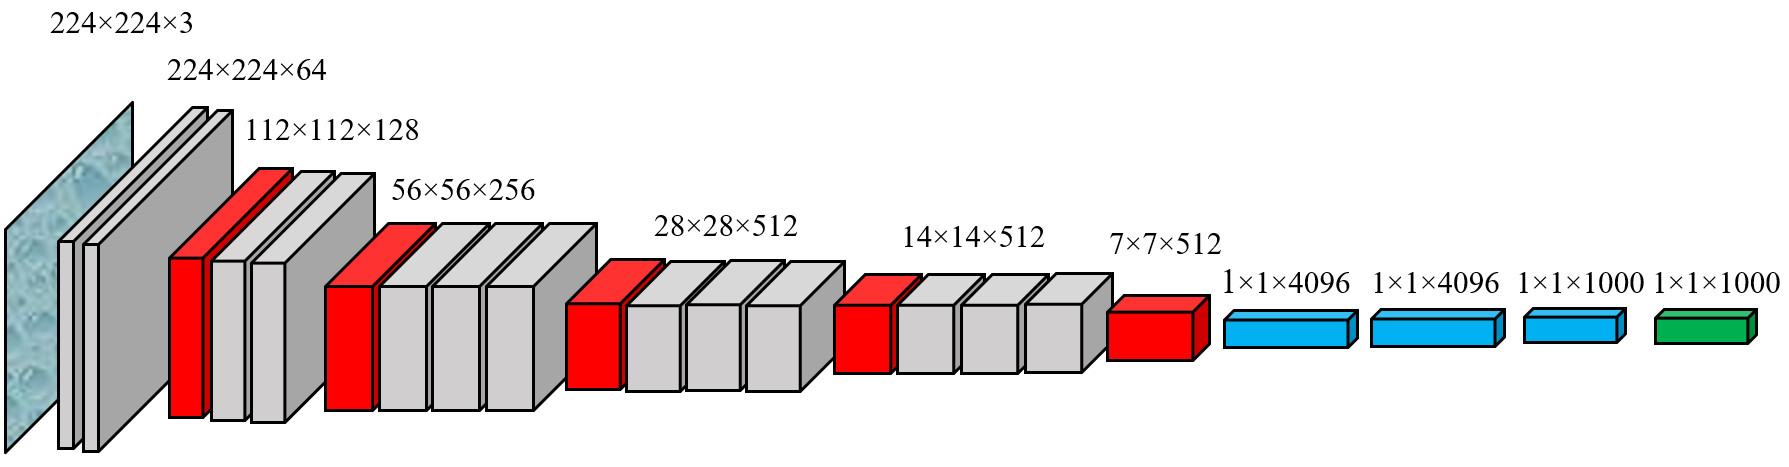
\includegraphics[width=\columnwidth]{30-activity/VGG_neural_network.png}
    \caption{VGG network. Grey: 3x3 convolution layers; red: pooling layers; blue: linear (or 1x1 convs) layers; green: softmax}. Each activation is described as $\text{Heigth} \times \text{Width} \times \text{Channels}$.
    \label{fig:vgg}
\end{figure}

However, those questions might not be that important after all. The \textbf{VGG} net  \citep{vgg} (Cf Figure \ref{fig:vgg}) uses only 3x3 convolutions, and doubles the number of channels after each pooling operation. Its simplicity encouraged researchers to invest time into simple designs with better fundamental principles rather that complex models.

\begin{figure}
    \centering
    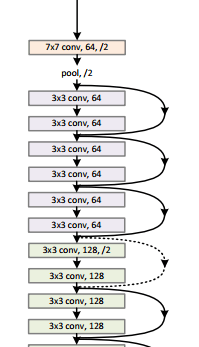
\includegraphics{30-activity/resnet.png}
    \caption{In ResNets, an identity path is added, so that the gradient can flow up to the first layers untouched. Figure from \cite{resnet}}
    \label{fig:resnet}
\end{figure}

\citet{resnet} observed that VGG nets could not be made very deep (no more than 20 layers). They hypothesized that the gradients quickly lose their supervision quality going back through the layers, failing to update the first layers. From this, they chose to design \emph{residual} networks, where convs compute additive residual transformations. The gradients can then flow unchanged along the identity path and keep its informative quality. The \textbf{Residual Network} (ResNet, cf Figure \ref{fig:resnet}) can go at least up to 1000 layers and still learn, despite reaching diminishing returns after 150 layers. The 50 layers variant is the most widely used because of its compute cost / performance tradeoff. ResNets were such an improvement that most of the following architectures integrated residual connections.

Note: Perceptrons are making their great comeback in image processing \citep{mlpmixer}, mostly through Transformers (Perceptrons with an attention mechanism) \citep{transformers,vit}. However, it does not invalidate what was said previously: while their performance scale better wrt big data quantity than \ac{SotA} \acp{CNN}, they perform worse than \acp{CNN} on smaller training sets (ImageNet-1k being considered "small" in this context). Indeed, despite limiting convnets at scale, the convolutional inductive biases embody some knowledge about natural images. Transformers based architectures need some more data to discover those invariances and close the gap, but are able to surpass \acp{CNN} with even more data. There are works trying to suggest inductive biases to vision transformers that the network can un-learn if needed, in order to make them perform on par or better than convnets in lower data regimes \citep{convit,coatnet} and always benefit from their scalability.

\subsection{Optimizers for Deep Learning}

Developing on optimizers is way beyond the scope of this work, but they cannot be kept unspoken of either. We briefly mention the main optimizers used for training deep networks.

\subsubsection{Stochastic Gradient Descent}

When gradient descent is done on a random subset of the training data, it becomes \ac{SGD}. \ac{SGD} is akin to walking the steepest direction in a valley in order to reach a minimum.

\ac{SGD} is slow and prone to underfitting as it has no mechanism to escape small local minima.

For weights $\theta$, gradient of the loss $\nabla J$, and hyperparameter learning rate $\alpha$:

\begin{equation}
    \theta := \theta - \alpha \nabla J
\end{equation}

\subsubsection{Stochastic Gradient Descent with Momentum}

Instead, \ac{SGD} is almost always used in its momentum variant. Taking the same analogy, \ac{SGDM} is like \emph{rolling} in the steepest direction. While we roll, we accumulate velocity $v$ that might help escape small local minima. Even if the valley is irregular, momentum helps escape those irregularities and reach the bottom. It adds a new momentum hyperparameter $\beta$.

\begin{equation}
\begin{split}
    v := & v + \beta \nabla J \\
    \theta := & \theta - \alpha v
\end{split}
\end{equation}

Another notable variant is Nesterov momentum. Here, the gradient evaluation is performed after the momentum step of the parameters, contrarily to SGDM.

\subsubsection{Adam}

Another family of optimizers, the \emph{adaptive optimizers}, made popular by \emph{\ac{Adam}} is said to be less sensitive to hyperparameters and especially to the learning rate. It works by scaling the learning rate by the rolling variance of the weight in the recent history. It introduces new hyperparameters, $\beta_1$ and $\beta_2$, respectively defaulted to 0.9 and 0.999. It also considers $t$, the number of the current iteration, and $\epsilon$, a constant for numerical stability.

\begin{equation}
\begin{split}
    m := & \beta_1 m + (1 - \beta_1) \nabla J \\
    v := & \beta_2 v + (1 - \beta_2) \nabla J \\
    \hat{m} := & m / (1 - \beta_1^t) \\
    \hat{v} := & v / (1 - \beta_2^t) \\
    \theta := & \theta - \alpha \hat{m} / \sqrt{\hat{v} + \epsilon}
\end{split}
\end{equation}

Despite its advantages in convergence speed and hyperparameters tuning, it has not fully took precedence over SGD as it converges to results only close to SGDM performance.

The literature explored many variants, including AdamW, RAdam, AdaMax, AMSGrad, AdaBelief, etc.

\subsection{Loss functions}

Any differentiable function that measures the error of the prediction can be used as a loss function. We will quickly lay out the most commonly used functions. 

\subsubsection{Cross-Entropy}

Cross-Entropy is used when the predictions are interpreted as the parameters of a categorical probability distribution. Cross-entropy measures the difference between two categorical distributions: the predicted distribution $p$ and the target distribution $\hat{y}$.

\begin{equation}
    \mathcal{L}(p, \hat{y}) = - \sum_i \hat{y}_i \log p_i
\end{equation}

In order to train a classifier, it optimizes the network's weights to predict a probability of 1 in the target class, reducing the other probabilities towards 0. This is strictly equivalent to maximizing the probability of the target class, or minimizing the negative log likelihood of the target class. The later formulation is preferred as it is computationally cheaper.

A neural network does not produce calibrated probability distributions on its own, but unconstrained scalars. They are often called \emph{logits}, as unnormalized log parameters of the categorical distribution, interpreted as the output of the logit function. Those logits $z_i$ can be be normalized into the categorical distribution parameters $o$ with the softmax function.

\begin{equation}
    o_i = \frac{\exp (z_i \tau)}{\sum_j \exp (z_j \tau)}
\end{equation}

Where $\tau$ is an optional \emph{temperature} parameter that controls the sharpness / entropy of the distribution.

While not being totally accurate, some people call the cross-entropy loss \emph{softmax loss}.

\subsubsection{Mean-Squared Error}

When trying to predict continuous values, one's default loss function choice is the L2 distance, or \ac{MSE}

\begin{equation}
    \mathcal{L}(y, \hat{y}) = (\hat{y}_i - y_i)^2
\end{equation}

\paragraph{Note: Numerical Considerations} When working with probabilities, computers might run into issues. Probabilities $p_i$ are often multiplied together and can become small, to the point where there could be representation issues with standard IEEE754 32 bits floats. For this reason, when possible, we instead manipulate log probabilities, taking advantage of this property:

\begin{equation}
    \prod_i p_i = \exp \sum_i \log p_i
\end{equation}

\subsection{Common datasets}

Some datasets are commonly used in computer vision in order to develop new techniques, compare models, or leverage knowledge from big datasets.

\subsubsection{MNIST}

MNIST \citep{mnist} is dataset of 28x28 greyscale images representing handwritten digits labeled with the ground truth digit. It contains 60k training pictures and 10k testing pictures. Classifying those digits is such a simple task that a SVM reaches 0.8\% error. In deep learning, MNIST is used as a sanity check for debugging or to introduce novel ideas, for instance with artificially introduced label noise.

\subsubsection{CIFAR-10/100}
\label{cifar10}

CIFAR-10 \citep{cifar10} contains 50k training 32x32 color images of 10 classes (airplane, automobile, bird, cat, deer, dog, frog, horse, ship, truck). There are 10k test images. This dataset is often used for developing new strategies. Optimizers, architectures, augmentations etc are often tested and calibrated on CIFAR-10 before before being battle-tested on ImageNet.

CIFAR-100 is similar but extended to 100 classes, 600 images each. It is not as commonly used as CIFAR-10.

\subsubsection{ImageNet-1K / ILSVRC12}

ImageNet (sometimes called ILSVRC for Image Large-Scale Visual Recognition Challenge) \citep{ILSVRC15,imagenet} is a large scale database of natural images crawled from the web, divided into 1k classes. It contains about 1M training pictures (~1k per class) and 50k testing images.

Since 2012, ImageNet has been the gold standard dataset for evaluation and comparison of classifiers. It is also commonly used to extract knowledge from natural images in order to build feature extractors or backbones for assembling models together \citep{imagenettransfer}. An expanded version of ImageNet, ImageNet-21k has been released. Models able to ingest lots of data are usually pretrained on it, before being tested on ImageNet-1k.

\section{\emph{\arr Practical Example}: A classifier for HActions}
\label{actionclf}

In this section we show how a standard image recognition problems can be solved with the tools laid out in this chapter. This is illustrated on activity recognition on the HActions dataset.

Activity recognition aims to identify what people are doing in still pictures or videos. At Hexaglobe, we are interested in activity tags in order to add metadata to our customers' content. They can be fed to search engines and recommender systems for more relevant results, as well as explicit categorization for a better user experience.

Most of the time, a still picture is enough to infer the activity: people sitting at a table with food are likely eating, people holding a microphone are most probably singing, etc.

\subsection{The model}

For industrial settings such as this one, training speed is more important than accuracy, so the tradeoff should favor iterative development. For this reason, I chose a ResNet-18 as our network. It has less parameters (11M) than the popular ResNet-50 (24M) for the sacrifice of few accuracy points.

As the HActions dataset (see section \ref{sec:hactions}) at most 2400 examples per class, training a model from scratch is likely to be suboptimal. In those situations where the dataset is relatively small, it helps to use \emph{transfer learning}. I chose to leverage a ResNet-18 from torchvision, pretrained on ImageNet-1k. The fact that both datasets are made of natural images suggests that the pretrained knowledge will be useful.


\subsection{Transfer Learning}

Natural images share common properties: neighboring pixels are correlated, the distribution of colors and brightness is not uniform, and some shapes occur frequently. When training a model on a large dataset such as ImageNet, the model would learn generic patterns, filters, shapes or objects that would be useful for other datasets or other tasks as well.

The parameters and architecture of the net is then kept untouched (or "frozen") but the last layer(s) that are trained on the new task. The frozen layers are used as a fixed feature extractor. This way, we only learn a small model from semantically rich features, instead of a bigger model from raw pixels. This allows to reuse natural images knowledge extracted from ImageNet. It helps preventing overfitting on meaningless spurious patterns in the case of small training sets, and to reuse knowledge for a different task. In addition to the performance advantage, this is much faster than training the whole thing as the features can be pre-computed only once.

After these last layer(s) have been retrained, it sometimes helps to \emph{fine tune} all the parameters of the model, by iterating a little more on the dataset, this time training the whole network with a very small learning rate. This allows the model to extract a few more useful or specific features that were not learned during the pretraining, while trying not to overfit . When possible, it helps to know how the base network has been trained as regularizers can improve ImageNet accuracy but reduce transferability \citep{imagenettransfer,crossentropytransfer}.

\subsection{Experiments}

\begin{table}[]
    \centering
    \begin{tabular}{|l|c|}
    \hline
        \textbf{Config} & \textbf{Test accuracy (\%)} \\
    \hline
        A: from random weights & 37.82 \\
    \hline
        C1: A + random flip & 43.87 (+10.05)\\
    \hline
        B: pretrained weights & 52.44 (+14.62) \\
    \hline
        C2: B + random flip & 55.67 (+3.23) \\
    \hline
        D: C2 + random crop & 55.67 (+0) \\
    \hline
        E: D + TrivialAugment & \textbf{58.19 (+ 2.52)} \\
    \hline
    \end{tabular}
    \caption{Test accuracy on HActions according to various configurations}
    \label{tab:hactivity_results}
\end{table}

In order to demonstrate what we laid down so far we run a quick set of typical experiments with a ResNet-18. All experiments are conducted with SGDM, weight decay (regularizing the square of the weights) is set to 1e-3, momentum is set to 0.9, batch size to 128, split across 4 GPUs. The learning rate is searched in \{0.3, 0.1, 0.01, 0.001, 0.0001\}. We train for 40 epochs. The \ac{lr} decays linearly from its initial value to 0 at the end of the training as \citep{lineardecay} shows this to be a sensible choice in common scenarios. The initial data augmentation includes random horizontal flipping and the pictures are resized to 128x227 which is unusual but keeps the 16:9 aspect ratio of the frames. We use a standard cross-entropy loss. A run takes about 1h.

We wish to verify and exemplify the benefits of a pretrained model and data augmentation, known to be among the top strategies to improve a natural images classifier.

The results, summarized in Table \ref{tab:hactivity_results}, show the power of pretraining and data augmentation, allowing performance boost with fast experiments. 

\paragraph{Config-A} trains from scratch. The best learning rate found is 0.1. It reaches an accuracy of 37.82\%.

\paragraph{Config-B} verifies that weights pretrained on ImageNet actually boost the accuracy. All the BatchNorm layers are kept in inference mode during training and the running statistics are not updated. The learning rate for all the layers but the last is set to 0 during the first 4 epochs and divided by 100 for the following iterations. The best learning rate found is 0.01. This significantly boosts the accuracy by 15\%, reaching 52.44\%.

\paragraph{Config-C} Config B is found to perform significantly better than A. Config-C adds random horizontal flipping of input images. Adding this transformation brings the random initialization (C1) to 43.87\%, and Config-B to 55.67\% (C2).

\paragraph{Config-D} adds inception-style random cropping to Config-C. It crops a random area from 80\% to 100\% of the image and resizes it to the input size.

\paragraph{Config-E} adds TrivialAugment (Section \ref{sec:trivialaugment}). The accuracy moves up to 58.19\%.

\subsection{Results and interpretation}

We trained a standard modern activity classifier from still pictures on HActions. Although 58\% may seem low, the dataset happens to be fairly small for classes that are loosely defined and somehow semantically hard to distinguish. For instance, if we were to classify dance move frames, the first and last few frames of each move, when the move starts and ends and is not clearly identifiable, this can legitimately be confused with no move at all. Upon manual inspection of the prediction on the test set, we indeed find that most of the errors can be attributed to ambiguity. The remaining errors can be largely attributed to a lack of data as they exhibit patterns not covered in training.

We would certainly solve many of those uncertainties by analyzing videos and neighbouring frames instead of independent frames, but that would come at a prohibitive cost. Instead we will consider those samples from a label noise perspective, hoping to construct a dataset without confusing training samples and reject ambiguous samples at inference time.

\section{Conclusion}

We demonstrated how the building blocks explained in this chapter (Figure \ref{fig:trainingloop}) can be assembled in order to train and utilize a learning algorithm. Pre-trained models for most used classification models are readily available and the data augmentation strategies are based on simple image manipulations. We show how one can leverage those for quick starting a project with little compute and data.

We trained a standard modern deep image classifier, leveraging battle tested techniques. Yet, the accuracy we obtained are usable for our use case, but somewhat below what can be expected from ImageNet capable models. We are facing problems that arise with "real world" usages: low data availability, labeling cost, ambiguity in samples and class semantics, etc. For instance, while ImageNet is a dataset of natural images, there are some peculiarities that might not be considered "real world", notably the data collection protocol that biased the data (keywords from search engines), or the fact that the class is an object centered and occupying the majority of the image surface.

In the next chapters, we apply the same standard classifier to the problem of face recognition, but quickly observe the same phenomenon: some data dependent problems are starting to arise, and need mitigation: there are some specific types of label errors that need to be fixed, the face extraction pipeline sometimes extracts non-face images, and the data bears its own set of hard features (very narrow demographics, extreme facial expressions, varying makeup, etc). The next chapter investigates dealing with label noise so as to mitigate the most damaging aspect of our training set: erroneous training samples.
\chapter{\emph{\arr Contribution}: Label noise for face recognition}
\label{chap:noise}

\section{Introduction}

Deep Learning systems have shown tremendous accuracy in image classification, at the cost of big, manually labeled, image datasets. Collecting such amounts of data can lead to labelling errors in the training set. Indexing multimedia content for retrieval, classification or recommendation can involve tagging or classification based on multiple criteria. In our case, we train face recognition systems for actors identification with a closed set of identities while being exposed to a significant number of distractors (actors unknown to our database). Face classifiers are known to be sensitive to label noise. We review recent works on how to manage noisy annotations when training deep learning classifiers, independently from our interest in face recognition.

Our client wishes to extract as much metadata as possible from their content. For the video content we host, identifying the actors is very valuable. Indeed, those videos have recurring actors that are worth identifying, among many unknown people that should be ignored. Users get to search for the content from the same actors, or similar actors. In order to extract these data, we build a face recognition system. We collect a dataset of face recognition with our celebrities. First we selected the 50 most popular celebrities on the platform and scrape pictures automatically from the internet, quickly verifying them manually resulting in 1k+ pictures per identity. In a second phase, we collect data for all the lesser known actors we wish to recognize. As those second-phase actors are less known, it is harder to find data for them, making automatic web scraping unreliable, and we shift to a strategy that is both more reliable and less time consuming. Human annotators are tasked to manually download between 10 and 100 pictures per identity, by descending order of popularity.

Bootstrapping and managing a large-scale dataset for face recognition requires either a lot of manual collection and labelling or scraping data from internet. Either way, the data is complex and the process is prone to error, and, when analyzing the data, we observe some recurrent error types:

\begin{itemize}
    \item some people might be lookalikes and end up mixed up by human annotators or web resources (eg Vin Diesel and Dwayne Johnson);
    \item some might share a similar name and get scraped together, either by an automatic process or a human annotator (like two women named Alexa);
    \item some others might appear frequently together and collecting one would probably get pictures of the others as well (like Eric Judor and Ramzy Bédia). It might also be hard to collect pictures where each person of interest is alone, and we might also end up collecting people sharing the shot.
\end{itemize}

For this reason, it became important to detect and mitigate label noise. I wrote a survey in order to learn the state of the art in detecting and handling label noise and its impact on image classification in general, keeping face recognition in mind.

This section is a contributed review paper published in ICME2020 \citep{MOIMOIMOIMOI}.

\section{Deep Learning Classification with Noisy Labels}
\label{sec:intro}

Learning a deep classifier requires building a dataset. Datasets in media are often situation dependant, with different looking sets or landscape or exhibiting various morphologies, even non-human for face recognition, especially in fantasy and sci-fi contexts. It becomes tempting to use search engines to build a dataset or sort large image sets based on metadata and heuristics. Those methods are not perfect and label noise is introduced.

It is widely accepted that label noise has a negative impact on the accuracy of a trained classifier. Several works have started to pave the way towards noise-robust training. The proposed approaches range from detecting and eliminating noisy samples, to correcting labels or using noise-robust loss functions. Self-supervised, unsupervised and semi-supervised learning are also particularly relevant to this task since those techniques require few or no labels.

In this chapter, we propose a review of recent research on training classifiers on datasets with noisy labels. We will reduce our scope to the data-dependant approaches estimating or correcting the noise in the data. It is worth mentioning that some works aim to make learning robust by designing new loss functions \citep{Bitempered,GeneralizedCE} without inspecting or correcting the noisy dataset in any way. Those approaches are beyond the scope of our study.

In the following sections, we first define label noise and summarize the different experimental setups used in the literature. We conclude by presenting recent techniques that rely on datasets with noisy labels. This work is inspired by \citep{NoiseSurvey}, extending it to deep classifiers.

\section{Overview of techniques}
All the techniques presented will vary in different ways defined and presented briefly in this section. They can differ on the noise model they build upon, and whether they handle open or closed noise, presented in subsection \ref{defs}, and based on \citep{NoiseSurvey}. Those noise models might need some additional human annotations in the dataset in order to be estimated, introduced in subsection \ref{annotations}. Subsection \ref{detection} will shortly enumerate approaches used for noisy samples detection, when needed. Once noisy samples have been detected, they can be mitigated differently, as outlined in subsection \ref{strategies}.

The various combinations taken by the approaches reviewed here are summed up in Table \ref{TheTableau}.

\subsection{Problem definition}

\label{defs}
\subsubsection{Models of label noise}

In the datasets studied here, we posit that each sample $x_i$ of a dataset has two labels: the true and unobservable label $y_i$, and the actual label observed in the dataset $\hat{y}_i$. We consider the label noisy whenever the observed label is different from the true label. We aim to learn a classifier $f(x_i)$ that outputs the true labels $y_i$  from the noisy labels $\hat{y}_i$. We denote a dataset $D$ as $D = \{(x_0, \hat{y}_0, y_0), ..., (x_n, \hat{y}_n, y_n)\}$ and $\hat{y}_i, y_i \in C$, the set of classes. As presented in \citep{NoiseSurvey} the dataset label noise can be modeled in three way in descending order of generality.

1) The most general model is called \textbf{Noise Not At Random} (NNAR). It integrates the fact that corruption can depend on the actual sample content and actual label. It requires complex models to predict the corruption that can be expected.

\begin{eqnarray}
P(\hat{y}=c|x)=\sum_{c' \in C} P(\hat{y}=c|y=c',x)P(y=c'|x)
\end{eqnarray}

2) \textbf{Noise At Random} (NAR) assumes that label noise is independent from the sample content and occurs randomly for a given label. Label noise can be modeled by a confusion matrix $\textbf{C} \in \mathbb{R}^{|C|\times|C|}$ that maps each true label to labels observation probabilities. It implies that some classes may be more likely to be corrupted. It also allows for the distribution of resulting noisy labels not to be uniform, for instance in naturally ambiguous classes. In other words, some pairs of labels may be more likely to be switched than others.

\begin{eqnarray}
P(\hat{y}=c|x) &=& P(\hat{y}=c)  \nonumber \\
~ &=& \sum_{c' \in C} P(\hat{y}=c|y=c')P(y=c')
\end{eqnarray}

3) The least general model, called \textbf{Noise Completely at Random} (NCAR), assumes that each erroneous label is equally likely and that the probability of an error is the same among all classes. For an error probability $E$, it corresponds to a confusion matrix with $P(E=0)$ on the diagonal and $P(E=1) / (|C| - 1)$ elsewhere. The probability of observing a label $\hat{y}$ of class $c$ among the set of all classes $C$ is

\begin{eqnarray}
P(\hat{y}=c|x) &=& P(\hat{y}=c)  \nonumber \\
%~ &=& P(\hat{y}=c|y=c)P(y=c) \nonumber \\
%~ && + \sum_{c' \in C \backslash \{c\}} P(\hat{y}=c|y=c')P(y=c') \nonumber \\
%~ &=& P(E=0)P(y=c) \nonumber \\
%~ && + \sum_{c' \in C \backslash \{c\}} \frac{P(E=1)}{|C|-1}P(y=c') \nonumber \\
~ &=& P(E=0)P(y=c) \nonumber \\
~ && + P(E=1)P(y \neq c)
\end{eqnarray}


\subsubsection{Closed-set, open-set label noise}

We distinguish \textbf{open-set} and \textbf{closed-set} noise. In closed-set noise, all the samples have a true label belonging to the classification taxonomy. For instance, a chair image is labeled "table" in a furniture dataset. In open-set noise this might not be the case, in the way a chair image labeled "chihuahua" in a dog races dataset has no correct label.

The second and third models discard open-set label noise by definition.

\subsection{Types of additional human annotations}
\label{annotations}

While training is done on a dataset with noisy labels, a cleaned test set is needed for evaluating the performance of the model. Those clean labels can be acquired from a more trusted yet limited source of data or via human correction.

We may also assume that a subset of the training set can be cleaned. A trivial approach in such cases, is to discard the noisy labels and perform semi-supervised learning using the validated ones and the rest of data as unlabeled. In noisy label training, one aims to exploit the noisy labels as well.

We can imagine a virtual metric, the complexity of annotation of a dataset, determined by factors such as the number of classes, the ambiguity between classes and the domain knowledge needed for labelling. A medical dataset could be hard to label even if it has only two classes while a more general purpose dataset could have a hundred classes that can easily be discriminated if they are all different enough. When the dataset is simple, true label correction can be provided without prohibitive costs.  When it is not, a reviewer can sometimes provide a boolean verification saying that the label is correct or not, which might be easier than recovering the true labels.

A dataset can then provide (1) no annotations, (2) corrected labels or (3) verified labels for a subset of its labels.

\subsection{Detecting the noisy labels}
\label{detection}

When working on a per-sample decision basis, we often perform noisy samples detection. There are several sources of information to estimate the relevance of a sample to its observed label. In the analyzed papers, four families of methods can be identified. Most of them manipulate the classifier learned, either through its performance or data representation.

1) Deep features are extracted from the classifier during training. They are analyzed with Local Outlier Factor (LOF) \citep{LOF} or a probabilistic variant (pLOF). Clean samples are supposed to be in majority and similar so that they are densely clustered. Outliers in feature space are supposed to be noisy samples.

2) The samples with a high training loss or low classification confidence are assumed to be noisy. It is assumed that the classifier does not overfit the training data and that noise is not learned.

3) Another neural network is learned to detect samples with noisy labels.

4) Deep features are extracted for each sample from the classifier. Some prototypes, representing each class, are learnt or extracted. The samples with features too dissimilar to the prototypes are considered noisy.

\subsection{Strategies with noisy labels}
\label{strategies}

Techniques mitigating noise can be divided in 4 categories. One is based on the NAR model, using statistical methods depending only on the observed labels. The three other methods use NNAR and need a per sample noise evaluation. These techniques are summed up in the Strategy column of Table \ref{TheTableau}.

1) One can \textbf{re-weight the predictions} of the model with a confusion matrix to reflect the uncertainty of each observed label. This is inherently a closed-set technique as the probability mass of the confusion matrix has to be divided among all labels.

2) Instead of re-weighting the predictions, we can \textbf{re-weight their importance} in the learning process based on the likelihood of a sample being noisy. Attributing a zero weight to noisy samples is a way to deal with open-set noise.

3) Supposedly erroneous samples can be \textbf{unlabeled}. The sample is kept and used differently, through semi-supervised or unsupervised techniques.

4) Finally, we can try to \textbf{fix the label} of erroneous samples and train in a classical supervised way.

\section{Experimental Setups}

While \textbf{CIFAR-10} \citep{cifar10} (section \ref{cifar10}) remains one of the most used datasets in image classification due to its small image sizes, relatively small dataset size, and not-too-easy taxonomy, it has clean labels that are unsuitable for our works. CIFAR-10 contains 60000 images evenly distributed among 10 classes such as "bird", "truck", "plane" or "automobile". It is still largely employed in noisy label training with artificial random label flipping, in a controlled manner to serve whichever method is shown. However, synthetically corrupting labels fails to exhibit the natural difficulties of noisy labels due to ambiguous, undecidable, or out of domain samples. MNIST \citep{mnist} can be employed under the same protocols, with a reduced size of classes of handwritten digits, each composed of 1000 images.

\textbf{Clothing1M} \citep{MassiveNoisy} contains 14 classes of clothes for 1 million images. The images, fetched from the web, contain approximately 40\% of erroneous labels. The training set contains 50k images with 25k manually corrected labels, the validation set has 14k images and the test set contains 10k samples. This scenario fits our low annotation complexity situation where labels can be corrected without too much difficulty, but the size of the dataset makes a full verification prohibitive.

\textbf{Food101-N} \citep{CleanNet} has 101 classes of food pictures for 310k images fetched from the internet. About 80\% of the labels are correct and 55k labels have a human provided verification tag in the training set. This dataset rather describes the high annotation complexity scenario where the labels are too numerous and semantically close for an untrained human annotator to correct them. However, verifying a subset of them is feasible.

Finally, \textbf{WebVision} \citep{WebVision} was scraped from Google and Flickr in a big dataset mimicking ILSVRC-2012 \citep{imagenet} (1k classes, 1.2M training samples), but twice as big. It contains the same categories, and images were downloaded from text search. Web metadata such as caption, tags and description were kept but the training set is left completely uncurated. A cleaned test set of 50k images is provided. WebVision-v2 extends to 5k classes and 16M training images.

When working on image data, all the papers used classical modern architectures such ResNet \citep{resnet}, Inception \citep{googlenet} or VGG \citep{vgg}.

\newcommand*\rot{\rotatebox{90}}

\begin{table*}[t]
\hspace*{-1cm}
\textwidth 180mm
\begin{tabularx}{\textwidth}{|p{3cm}||c|c|p{1cm}|p{1.5cm}||c|c|c||X|X|X|X||X|X|X|X|}
\hline
~ & \multicolumn{4}{c||}{\textbf{Strategy}} & \multicolumn{3}{c||}{\textbf{Annotations}} & \multicolumn{4}{c||}{\textbf{Detection}} & \multicolumn{4}{c|}{\textbf{Datasets}}\\
\hline
    ~ & \rot{\textbf{Reweight predictions}}\rot{(NAR, Closed-set)} & \rot{\textbf{Reweight or remove samples}}\rot{(NNAR, Open-set)} & \rot{\textbf{Unlabel samples}}\rot{(NNAR, Open-set)} & \rot{\textbf{Fix labels}}\rot{(NNAR, Closed-set)} & \rot{\textbf{No correction}} & \rot{\textbf{Corrected labels}} & \rot{\textbf{Verified labels}} &
    \rot{\textbf{Local Outlier Factor}} & \rot{\textbf{High loss / Low confidence}} & \rot{\textbf{Model}} & \rot{\textbf{Similarity to prototypes}} & \rot{\textbf{CIFAR-10 / MNIST}}\rot{(Synthetic noise)} & \rot{\textbf{Food-101N}}\rot{(Verified labels)} & \rot{\textbf{Clothing1M}}\rot{(Corrected labels)}
    & \rot{\textbf{WebVision}}\rot{(Raw labels)}\\
\hline
\hline
% reweight pred

%reweight s
NLNL & ~ & \checkmark & ~ & negative labels & \checkmark & ~ & ~ & ~ & \checkmark & ~ & ~ & \checkmark & ~ & ~ & \\
\hline
Iterative Noise Filtering & ~ & ~ &  without \newline entropy loss & with entropy loss & \checkmark & ~ & ~ & ~ & \checkmark & ~ & ~ & \checkmark & ~ & ~ &\\
\hline

Ren et al, 2018 \citep{Reweight} & ~ & \checkmark & ~ & ~ & \checkmark & ~ & ~ & ~ & ~ & \checkmark & ~ & \checkmark & ~ & ~ & \\
\hline
Iterative learning & ~ & \checkmark & ~ & ~ & \checkmark & ~ & ~ & \checkmark & ~ & ~ & ~ & \checkmark & ~ & ~ & \\
\hline

NLNN & \checkmark & ~ & ~ & \checkmark & \checkmark  & ~ & ~ & ~ & ~ & ~ & ~ & \checkmark & \multicolumn{3}{c|}{\& TIMIT} \\
\hline
Hendrycks et al, 2018 \citep{Trusted} & \checkmark & ~ & ~ & ~ & ~ & \checkmark & ~ & ~ & ~ & ~ & ~ & \checkmark & \multicolumn{3}{c|}{\& NLP} \\
\hline

Deep Self-Learning & ~ & ~ & ~ & \checkmark & \checkmark & ~ & ~ & ~ &  ~ & ~ & \checkmark & ~ & \checkmark & \checkmark &\\
\hline
CleanNet & ~ & \checkmark & ~ & ~ & ~ & ~ & \checkmark ~ & ~ & ~ & \checkmark & \checkmark & ~ & \checkmark & \checkmark & \\
\hline

Xiao et al, 2015 \citep{MassiveNoisy} & \checkmark & ~ & ~ & ~ & ~ & \checkmark & ~ & ~ & ~ & \checkmark & ~ & ~ & ~ & \checkmark & \\
\hline
CurriculumNet & ~ & \checkmark & ~ & ~ & \checkmark & ~ & ~ & ~ & \checkmark & ~ &  ~ &  ~ &  ~ &  ~ &  \checkmark \\
\hline

Co-Mining & ~ & \checkmark  & ~ & ~ & \checkmark  & ~ & ~ & ~ & \checkmark & ~ & ~ & \multicolumn{4}{c|}{face rec}\\
\hline
\end{tabularx}
\caption{Approaches according to annotations in the dataset. Notes: TIMIT is a speech to text dataset, "NLP" is a set of natural language processing datasets (Twitter, IMDB and Stanford Sentiment Treebank), "face rec" denotes classical face recognition datasets (LFW, CALFW, AgeDB, CFP)}
\label{TheTableau}
\end{table*}


\section{Approaches}
\label{Approaches}

\subsection{Prediction re-weighting}

Given a softmax classifier $f(x_i)$ for a sample $x_i$, prediction re-weighting mostly implies estimating the confusion matrix $\textbf{C}$ in order to learn $\textbf{C}^Tf(x_i)$ in a supervised fashion with the noisy labels. Doing so will propagate the labels' confusion in the supervising signal to integrate the uncertainty about label errors. The main difference between the approaches lies in the way $\textbf{C}$ is estimated.

In \textbf{\acf{NLNN}} \citep{NLNN}, noisy labels are assumed to come from a real distribution observed through a noisy channel. The algorithm performs an iterative Expectation Maximization algorithm. In the Expectation step, correct labels $y_i$ are guessed through $\textbf{C}^Tf(x_i)$ while in the Maximization step, $\textbf{C}$ is estimated from the confusion matrix between guessed labels $\tilde{y}_i$ and dataset labels $\hat{y}_i$. Finally, $f(x_i)$ is trained on guessed labels $\tilde{y}_i$. The process is repeated until convergence.

Taking a more direct approach, \textbf{(Xiao et al, 2015)} \citep{MassiveNoisy} directly approaches $\textbf{C}$ by manually correcting the labels of a subset of the training set. Then, a secondary neural network $g(x_i)$ is defined, giving to each sample a probability $P(z_{1,i}, z_{2,i}, z_{3,i} | x_i)$ of being either ($z_1$) noise free, that is $\hat{y}_i = y_i$, ($z_2$) victim of completely random noise (NCAR), ie $P(\hat{y}_i | y_i) = (U-I)y_i$ such that the matrix $U$ is uniform and all rows of $U-I$ sums to 1, or ($z_3$) confusing label noise (NAR), $P(\hat{y}_i | y_i) = \textbf{C}^T\hat{y}_i$. Finally, $f(x_i)$ is trained on the noisy labels so as to minimize $L_\text{CE}(z_{1i} f(x_i) + z_{2i}(U-I)f(x_i) + z_{3i}\textbf{C}^Tf(x_i), \hat{y}_i)$ with $L_\text{CE}$ the cross entropy loss function.

\textbf{(Hendrycks et al, 2018)} \citep{Trusted} first train a model on the dataset with noisy labels. This model is then tested on a corrected subset and its predictions errors are used to build the confusion matrix $\textbf{C}$. Finally $f(x_i)$ is trained on the corrected subset and $\textbf{C}^Tf(x_i)$ is trained on the noisy subset.

\subsection{Sample importance re-weighting}

For a softmax classifier $f(x_i)$ trained with a loss function such as cross-entropy $L_{\text{CE}}$, sample importance re-weighting consists in finding a sample weight $\alpha_i$ and minimizing $\alpha_iL_\text{CE}(f(x_i), \hat{y}_i)$. For a value $\alpha_i$ close to 0, the example has almost no impact on training. $\alpha_i$ values larger than 1 emphasize examples. If $\alpha_i$ is exactly 0, then it is analogous to removing the sample from the dataset.

\textbf{Co-mining} \citep{CoMining} investigates face recognition where correcting labels is unapproachable for a large number of identities, and most likely a situation of open-set noise. Two neural nets $f_1$ and $f_2$ are given the same batch. For each net, the losses $l_{1i} = L(f_1(x_i), \hat{y}_i)$ and $l_{2i} = L(f_2(x_i), \hat{y}_i)$ are computed for each sample and sorted. The samples with the highest loss for both nets are considered noisy and are ignored. The samples $s_{1,i}$ and $s_{2,i}$ that have been kept by $f_1$ and $f_2$ are considered clean and informative: both nets agreed. Finally, the samples kept by only one net are considered valuable to the other. Backpropagation is then applied, with clean faces weighted to have more impact, valuable faces swapped in order to learn $f_1$ with $s_{2,i}$ and $f_2$ with $s_{1,i}$, and low quality samples are discarded.

\textbf{CurriculumNet} \citep{CurriculumNet}
trains a model on the whole dataset. The deep features of each sample are extracted, and from the Euclidean distance between features vectors, a matrix is built. Densities are estimated, 3 clusters per class are found with k-means, and ordered from the most to least populated. Those three clusters are used for training a classifier with a curriculum, starting from the first with weight 1, then the second and third, both weighted $0.5$.

\textbf{Iterative learning} \citep{IterativeLearning} chooses to operate iteratively rather than in two phases like CurriculumNet. The deep representations are analyzed throughout the training with a probabilistic variant of Local Outlier Factor \citep{LOF} for estimating the densities. Local outliers are deemed noisy. The unclean samples importance is reduced according to their probability of being noisy. A contrastive loss working on pairs of images is added to the cross entropy. It minimizes the euclidean distance between the representation of samples considered correct and of the same class, and maximizes the Euclidean distance between clean samples of different class or clean and unclean samples. The whole process is repeated until model convergence.

We can also employ meta-learning by framing the choice of the $\alpha_i$ as values that will yield a model better at classifying unseen examples after a gradient step. \textbf{(Ren et al, 2018)} \citep{Reweight} performs a meta gradient step on $L=\alpha_iL_\text{CE}(f(x_i), \hat{y}_i)$ then evaluate the new model on a clean set. The clean loss is backpropagated back through $L$, for which the gradient $\eta$ gives the contribution of each sample to the performance of the model on the clean set after the meta step. By setting $\alpha_i = \text{max}(0, \eta_i)$, the samples that impacted the model negatively are discarded, and the positive samples get an importance proportional to the improvement they bring.

\textbf{CleanNet} \citep{CleanNet} learns what it means for a sample to come from a given class distribution, utilizing a correct / incorrect tag provided by human annotators. A pretrained model extracts deep features of the whole dataset. Then, they run a per-class K-Means, and find the images with features closest to the centroids as a set $v_c$ of reference images for that class $c$. A deep model $g(v_c)$ encodes the set into a single prototype. A third deep model $h(x_i)$ encodes the query image $x_i$ in a prototype. We learn to maximize $w_{ci}=\cos(g(v_{c}), h(x_{i}))$ if $x_i$ has a correct class $c$, and to minimize it otherwise. This relevance score is used to weigh the importance of that sample when training a classifier with $\max(0, w_{\hat{y}_i}) L_{\text{CE}}(f(x_i), \hat{y}_i)$.

Instead of getting a consistent wrong information from an erroneous label, \textbf{NLNL} \citep{NLNL} (not to be confused with NLNN) samples a label $\Tilde{y}_i \neq \hat{y}_i$ and uses negative learning, a negative cross-entropy version that minimizes the probability of $\Tilde{y}_i$ for $x_i$. As the number of classes grows, the more likely the sampled label $\Tilde{y}_i$ is indeed different of $y_i$ and noise is mitigated, despite being less informative. Then only samples with a label confidence above $1/|C|$ are kept and used negatively in a second phase called Selective Negative Learning (SelNL). Finally, examples with confidence over a high threshold (0.5 in the paper) are used for positive fine-tuning with a classical cross entropy and their label $\hat{y}_i$.

\subsection{Unlabeling}

\textbf{Iterative Noise Filtering} \citep{IterativeNoiseFiltering}:
A model is trained on the noisy dataset. An exponential moving average estimate of this model is then used to analyze the dataset. Samples classified correctly are considered clean, while the label is removed for those classified incorrectly. The model is further trained with both a supervised and unsupervised objective for labeled and unlabeled samples. The samples with labels are used with a cross entropy loss. For each unlabeled sample, we maximize $\max_c f(x_i)_c$ in order to reinforce the model's prediction, while maximizing the entropy of the predictions over the whole batch to avoid degenerate solutions. After each epoch, the dataset's labels are evaluated again according to the average model. 

\subsection{Label fixing}

A few methods already listed above try to fix the labels as part of their approach. While listed as a sample re-weighting method, \textbf{NLNL} \citep{NLNL} also employs a sort of label fixing procedure by using the negative labels. Similarly, NLNN \citep{NLNN} attempts to fix the labels while estimating the confusion matrix. Finally, \textbf{Iterative Noise Filtering} \citep{IterativeNoiseFiltering}, assumes that the class with the highest prediction for the unlabeled examples is correct.

\textbf{Deep Self-Learning} \citep{SelfLearning} learns an initial net on noisy labels. Then, deep features are extracted for a subset of the dataset. A density estimation is made for each class and the most representative prototypes are chosen for each cluster. The similarity of all samples to each set of prototypes is computed to re-estimate correct labels $\Tilde{y}_i$. The model training continues with a double loss balancing learning from the original label or the corrected one $L=\lambda L_\text{CE}(f(x_i), \hat{y}_i) + (1-\lambda)L_\text{CE}(f(x_i), \Tilde{y}_i)$ with hyper-parameter $\lambda \in [0,1]$. We iterate between label correction and weighted training until convergence. Note that contrarily to sample weighting techniques that weigh the contribution of each sample in the loss, all samples have an equal importance, but we place a cursor as a hyper-parameter to balance between contribution from the noisy labels and corrected labels.

\section{Discussion}

Those approaches cover a wide variety of use cases, depending on the dataset: whether is has verified or corrected labels or not, and the estimated proportion of noisy labels. They all have different robustness properties: some might perform well in low noise ratio but deteriorate quickly while others might have a slightly lower optimal accuracy but do not deteriorate as much with high noise ratio.

Re-weighting predictions performs better on flipped labels rather than uniform noise as shown in the experiments on CIFAR-10 in \textbf{Hendrycks et al, 2018} \citep{Trusted}. As noise becomes close to a uniform noise, the entropy of the confusion matrix $\textbf{C}$ increases, labels provide more diffused information, and prediction re-weighting is less informative. CIFAR-10 being limited to 10 classes, NLNN \citep{NLNN} is shown to scale with a greater number of classes on TIMIT.

Noisy samples re-weighting scales well: CurriculumNet \citep{CurriculumNet} scales in number of samples and classes as the experiments on WebVision shows, Co-Mining \citep{CoMining} is able to scale to face recognition datasets and open-set noise at the expense of training two models, CleanNet generalizes its noisy samples detection by manually verifying a few classes.

However, NLNL \citep{NLNL} may not scale as the number of classes grows: despite having negative labels that are less likely to be wrong, they also become less informative. 

We can expect unlabeling techniques to grow as the semi-supervised and unsupervised methods gets better, since any of those can be used once a sample had its label removed. One could envision utilizing algorithms such as MixMatch \citep{MixMatch} or Unsupervised Data Augmentation \citep{UDA} on unlabeled samples.

Similarly, the label fixing strategies could benefit from unsupervised representation learning to learn prototypes that makes it easier to discriminate hard samples and incorrect samples. Deep self-learning \citep{SelfLearning} is shown to scale on Clothing1M and Food-101N. It would be expected that those approaches become less accurate as the number of classes grows or the classes get more ambiguous. Some prior knowledge or assumptions about the classes could be used explicitly by the model. Iterative Noise Filtering \citep{IterativeNoiseFiltering} in its entropy loss assumes that all the classes are balanced in the dataset and in each batch.

\section{Conclusion}

We explored the situation where a deep classifier has to be learnt on data with label noise, that is, containing erroneous target labels. We explored the literature and showed that the approaches can be sorted into four main categories: reweighting predictions using a noise model, reweighting the importance of training samples based on their assessed probability of having a wrong label, unlabel the suspicious samples and use them with unsupervised training, or fixing the suspicious labels with new guesses.

Training a deep classifier using a noisy labeled dataset is not a single problem but a family of problems, instantiated by the data itself, noise properties, and provided manual annotations if any. As types of problems and solutions will reveal themselves to the academic and industrial deep learning practitioners, deciding on a single metric, a more thorough and standardized set of tests might be needed. This way, it will be easier to answer questions about the use of domain knowledge, generality, tradeoffs, strengths and weaknesses, of noisy labels training techniques depending on the use-case.

In the face recognition system that we are building, label noise have varying causes: persons with similar names; confusion with lookalikes; related persons that appear together; erroneous faces detected on signs or posters in the picture; errors from the face detector that are not faces; and random noise. All those situations represent label noise with different characteristics and properties that must be handled with those algorithms. We believe those issues are more general than this scenario and find an echo in the broader multimedia tagging and indexing domain.

From this study we mainly keep that samples with label errors produce higher losses than correctly labeled ones. The next chapter will explore how to leverage this in order to manually curate our training set. Furthermore, as we will show, a face recognition dataset contains pictures of many identities, but can also include pictures that do not belong to any of the known identities. This situation is reminiscent of the open-set label error (when the correct label does not belong to any of the known label) or unlabeled samples.
\chapter{Face Recognition}
\label{sec:facerec}

As previously mentioned, a face recognition system embedded on the customer's platform would extract metadata that could be interesting for our recommendation engine and valuable for the user experience.

We will first highlight how our use case is different from the general case, then present how face recognition is usually tackled, and finally explore our system currently in production. We will emphasize our contributions: a new metric-learning loss function, the threshold-softmax loss, and a study of several methods for exploiting unlabeled faces during training.

\subsection{Industrial setting}

In our industrial setting, we wish to identify some people of interest ("VIPs") among many unknown people in videos with unconstrained facial pose, illumination, expression and occlusion. The set of identities of interest is known ahead of time but a lot of the input pictures, if not most, are unknown people that must be rejected by the system. This particular setting makes this an instance of a subject-dependent open-set protocol, which we observe to be an understudied case, not even considered in Wang et al (2021) \cite{survey} (Figure \ref{fig:survey}).

We believe this setting is particularly common under some industrial settings in which we are interested in some people, like celebrities, for which we can acquire datasets if needed, among many unknown test-time distractors. One such example would be reidentifying famous YouTubers in fan compilations, clips or video reuses. Another would be to reidentify famous actors in movies among extras.

We call \emph{distractors} faces whose identity is unknown to the system. It is expected that the system rejects those faces and is aware that they are unknown. The presence or absence of distractors is what differentiates open-set and close-set settings.

Hexaglobe's Face Recognition system has some specificities compared to the algorithms laid in the literature:

\begin{enumerate}
    \item Contrarily to most, this work is focused on identifying a known set of identities among distractors. Most works instead deal with verifying if a query face is the same person as a key face, for instance, verifying if the person at the customs is the same as the one on the passport being presented.
    
    \item Most works on classifiers focus on having a correct best guess, but this system does not have to make a prediction for every input. The model rejecting some inputs because of uncertainty is a better outcome than a failed prediction. Knowing that we don't know is crucial here.

    \item Our work is deployed at scale where it analyzes hundreds of user uploaded videos per day. Those videos present real world faces in the wild, with occlusions, variable lighting conditions, image resolution, quality and scale, not properly aligned, sometimes with extreme facial poses, making this data more challenging than most used datasets currently used in publications \citep{celeb1m}.
\end{enumerate}

However, our setting allows some relaxations :

\begin{enumerate}
    \item As a public video platform using the system for tagging videos with identities for search improvements, we are only interested in tagging the most popular people. These people can be decided ahead of time and our problem becomes a semi-open set face recognition problem: the set of identities to recognize is known ahead of time but there are unknown distractors to reject.

    \item All errors are not equal. It is more harmful to add a wrong tag than to miss one. In our case, precision is more important than recall. This makes it possible, even needed, to let the model express its lack of confidence and not act on uncertain predictions.

    \item As we are interested in overall video tagging and not per frame tagging, per frame errors are not harmful if they can be smoothed out.
\end{enumerate}

Besides, considering the volume of existing videos (approx 8M) and the number of new uploads per day, processing a video should not take more than 5 minutes. In order to guarantee this processing time, we extract 300 frames evenly spaced throughout the video.

Finally, as our system is meant to have a quickly growing set of persons of interest, we favor fast iterations, both in model training time and time needed to add a subject to the set of known persons.

\section{Standard systems}

Face recognition (FR) systems based on deep learning have been under heavy research these past years. As outlined in Wang et al (2021) \cite{survey}, FR systems can be characterized by two major features: whether we expect the train and test sets to contain the same identities or not (subject-dependent vs subject-independent protocol), and the evaluation task: verification (whether a picture matches the identity of another), closed-set identification (all input test identities are known to the system) and open-set identification (some test inputs does not belong to any known identity and must be rejected).

We observe that a lot of work went into the subject-independent closed-set protocol thanks to MegaFace \cite{megaface}. Contrarily, the subject-dependent protocol has mostly been considered in the closed-set evaluation and deemed to be solved with a simple image classifier, not receiving much attention. Figure \ref{fig:survey} does not even consider other settings.

\begin{figure}
    \centering
    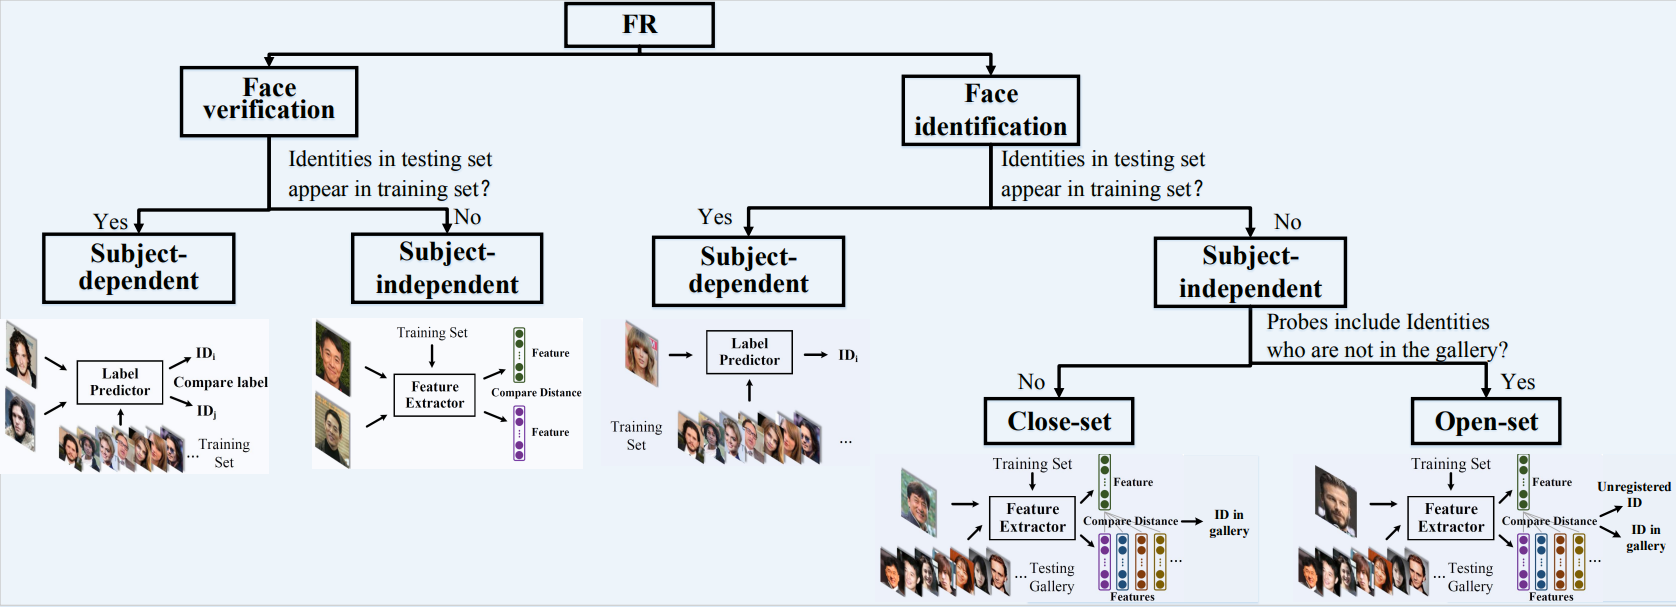
\includegraphics[width=\columnwidth]{50-files/survey.png}
    \caption{Figure 17 from Wang et al (2021) \cite{survey}. The comparison of different training protocol and evaluation tasks in FR. In terms of training protocol, FR can be classified into subject-dependent or subject-independent settings according to whether testing identities appear in training set. In terms of testing tasks, FR can be classified into face verification, close-set face identitification, open-set face identification.}
    \label{fig:survey}
\end{figure}

\subsection{Open-set/closed-set and subject-dependent/subject-independent recognition}

As explicited in Figure \ref{fig:survey}, face recognition systems, when focusing on the task of open-set verification, have to decide whether two pictures of people unseen during training time are the same person or not. In order to generalize to unseen identities, the systems are trained under a similarity learning objective to produce dense semantic face representations that should be similar for same identities and dissimilar for different identities under cosine or Euclidean distance (for the general case). The Triplet Loss \cite{triplet,triplet-face} explicitly enforces those properties with a negative and positive pair relative to an anchor face. While it marked the beginning of scalable face recognition systems, the long training time drove the community to more data-efficient and time-efficient techniques. Present state-of-the-art approaches such as SphereFace \cite{sphereface}, CosFace \cite{cosface}, ArcFace \cite{arcface}, AdaCos \cite{adacos} mostly build on classification losses such as Cross-Entropy with margin and representation constraints (such as normalizing L2 norm). Current datasets  for those approaches have about 10k of identities in order to learn good discriminative features that generalize well (Megaface \cite{megaface}, VGGFace2 \cite{vggface2}, MS1M \cite{celeb1m}, ImdbFace \cite{imdbface}, IJB-{A,B,C} \cite{ijb-a, ijb-b, ijb-c}).

Those representations are then extracted from reference images and compared independently with the input image’s representation.

\begin{figure}
    \centering
    \includegraphics[width=\columnwidth]{50-files/facerec1.pdf}
    \caption{Training of classification-based metric learning algorithm. The algorithm is trained to classify faces in different identities, with a margin in softmax and representation constraints.}
    \label{fig:facerec1}
\end{figure}

\begin{figure}
    \centering
    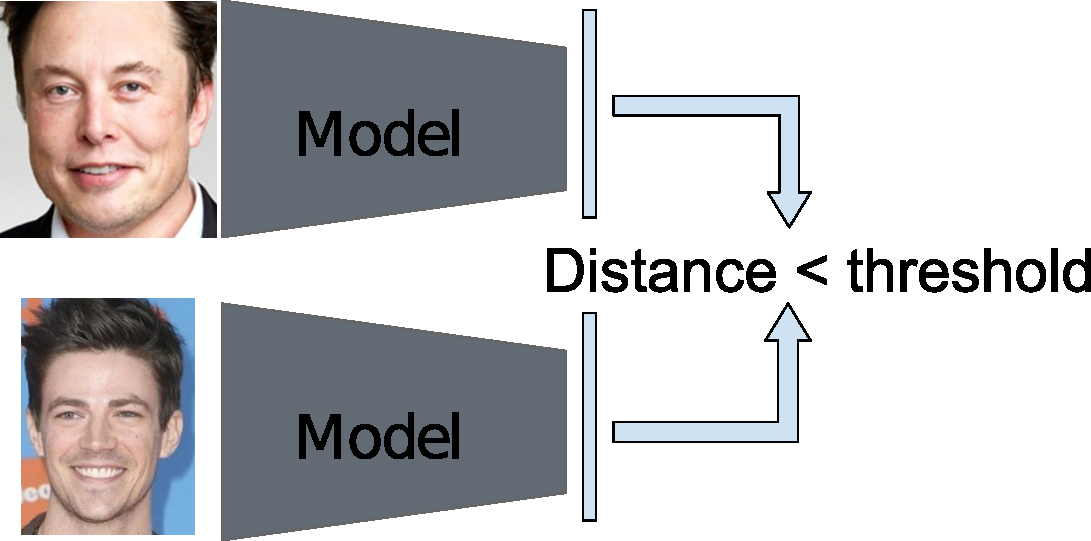
\includegraphics[width=\columnwidth]{50-files/facerec2.pdf}
    \caption{Test time usage of feature vectors. Two images’ representations are compared under a distance metric. A distance under a predefined threshold indicates the same identity.}
    \label{fig:facerec2}
\end{figure}

When tasked to identify, the input image (the “probe”) is encoded in a feature vector and compared to all the encoded reference picture vectors (the “gallery”), aiming for minimum distance on the correct identity. This strategy has some shortcomings outlined in \cite{ijb-a}: it is unclear how to aggregate various feature vectors from several images of the same identity, and current systems are not precise enough to reject all the images in the gallery for unknown probe identity when the gallery has many pictures, triggering false detections. For testing, LFW \cite{lfw} is a common test set as well.

\section{Metric learning}

In order to generalize to unseen faces, FR systems are usually seen as a metric learning (or similarity learning) problem instance. In general, metric learning aims to learn an embedding space that is semantically meaningful wrt to a chosen distance function (usually euclidean or angular).

Under this framework, we aim to obtain a neural network embedding a face into similar vectors for the same person and dissimilar vector for different people. The similarity measure is often euclidean or angular.

\subsection{Triplet loss}

The most direct translation of this goal is the Triplet Loss \citep{triplet-face,tripletloss,triplet}. For a neural net $f$ that takes a face as an input and outputs a vector, and a distance function $d$, we want to minimize

\begin{equation}
    \mathcal{L} = d(f(A_i), f(A_j)) - d(f(A_i), f(B_k))
\end{equation}

where $A_i$ and $A_j$ are two different pictures of a person A, and $B_k$ is a picture of a different person B.

While this work, this requires a lot of time to converge.

\subsection{Softmax}

Posing the problem as a classification task allows to leverage the efficiency of the cross-entropy loss and the discriminative capability of neural networks. In order to frame $f$ as a classifier, we need to define

\begin{equation}
    h(x) = \text{softmax}(f(x) \cdot W^T)
\end{equation}

Here, $W$ is a learnable $k\times d$ matrix where $k$ is the number of identities to classify and $d$ is the dimension of the embedding row vector produced by $f$. The $i$th row of $W$ can be interpreted as the prototypical embedding for class $i$.

At inference time, $W$ is discarded and a distance function is used to compare the embeddings. It is hoped that $f$ was trained on enough identities in order to make a rich, semantically meaningful vector space. During training, as the embeddings were discriminated with a linear classifier, a parameter-free distance function should be able to discriminate embeddings from people not seen during training.

\subsection{L2-softmax}
\newcommand{\vnorm}[1]{\langle #1 \rangle}

Vanilla softmax has some notable drawbacks: it does not enforce positive pairs to remain together and negative pairs further; it is biased towards the training distribution unbalance; and uncertain samples produce decisions with low confidence that are poorly penalized.

\citet{l2softmax} (Figure \ref{fig:tsm}a) proposes to fix all of those by enforcing a L2 constraint on both the output vector of $f$ and each row of $W$. Instead of maximizing the softmax output with maximum inner product between the correct row of $W$ and $f(x)$, this aims to maximize (minimize) the cosine similarity between the correct (incorrect) row of $W$ and $f(x)$. If we accept the notation $\vnorm{n}$ for a matrix $n$ with each row vector normalized to unit length, the L2-softmax is:

\begin{equation}
    \label{eq:l2sm}
    h(x) = \text{softmax}(s \vnorm{f(x)} \cdot \vnorm{W}^T ) = \text{softmax}(s \cos(f(x), W)) = \text{softmax}(s \cos \theta)
\end{equation}

where the scalar $s$ can be either interpreted as a radius or the temperature of the softmax. The higher the $s$, the more the softmax will resemble a hard $\text{argmax}$. As $\cos$ is bounded in [-1; 1], it is necessary to control the sharpness of the softmax with a temperature in order to control the gradient magnitude. $\theta$ is the vector of the angles between $f(x)$ and each row of $W$.

Note that in the equation above, $\cos$ is applied independently to each row of $W$ and $f(x)$, also making $\theta$ a vector of size $k$ representing the angles between $f(x)$ and each row of $W$.

\subsection{ArcFace}

ArcFace \cite{arcface} (Figure \ref{fig:tsm}b) builds on this by enforcing a margin between classes. The L2-softmax (Eq. \ref{eq:l2sm}) emits a valid high probability as soon as $f(x)$ has its smallest angle with the prototype of the correct class in $W$. They thought this was not enough and wanted to add another guarantee, that small perturbations to $f(x)$ due to input distribution shifts or hard samples would not be predicted as another class. As such, they add an hyperparameter margin $m$ in the equation to repel the embedding by $m$. By adding $m$ radians to the angle of the correct class the angular distance with other classes is forced to be greater than the margin:

\begin{equation}
    h(x) = \text{softmax}(s \cos(\theta + m\hat{y}))
\end{equation}

where $\hat{y}$ is a $k$ dimensional row vector one-hot encoding the target class.

Some other margins were proposed prior to ArcFace such as \citep{sphereface} or \citep{cosface} but showed lesser accuracy at test time.

\section{\arr \emph{Contribution}: Threshold-Softmax}

\subsection{Principle}

\begin{figure}
    \centering
    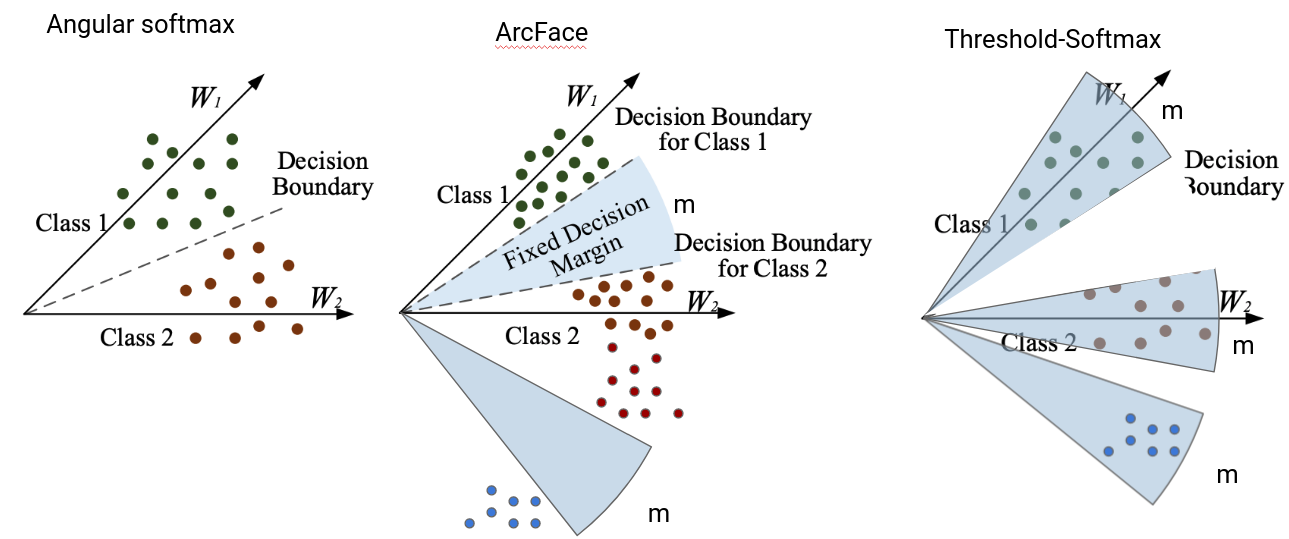
\includegraphics[width=\columnwidth]{50-files/download.png}
    \caption{Comparison of the angular softmax, ArcFace and the proposed Threshold-Softmax. In ArcFace, the margin (in blue) is fixed but the width of the arcs of each class can be arbitrarily wide (or narrow), since there is no constraint on them. In threshold-softmax, there are no enforced margins but the decision boundaries have a fixed width. An artificial class is predicted outside of those trusted cones.}
    \label{fig:tsm}
\end{figure}

ArcFace constrains the representation so that the angular distance to an incorrect class is at least of size $m$, but does not enforce any absolute requirement on the intra-class angles. I wanted to explore the opposite view and constrain the representation vector in the other way, so that the angle between samples of the same class is \emph{at most} $m$, making it an absolute requirement.

I achieved this by concatenating an artificial entry $\cos(m)$ to $\theta$. We say this entry has class $\Omega$. If all the angles in $\theta$ are greater than $m$, then this artificial entry is maxed out by the softmax function, leading to a high loss until the correct angle is finally smaller than $m$. $m$ being a hyperparameter. The loss function can be expressed as:

\begin{equation}
    h(x) = \text{softmax}(s [\cos(f(x),W); \cos m])
\end{equation}

Figure \ref{fig:tsm} highlights the difference with standard angular softmax, ArcFace, and Threshold-Softmax.

\section{Evaluation}

In the subject independent scenario, the dataset LFW \citep{lfw} test set is commonly used to assess the quality of face representation. It consists of 6k image pairs, half being faces of the same identity, half being of different ones. The model has to decide whether a pair of pictures belong or not to the same identity.

State-of-the-art accuracy on this set surpassed 99\% which drove the creation of newer and harder sets.

FGLFW \citep{fglfw} reuses pictures from LFW but selected harder pairs. DeepFace has an accuracy of 92.87\% on LFW but 78.78\% on FGLFW.

The Megaface challenge \citep{megaface} extends this beyond pairs. They propose an input "probe" picture and a gallery of "candidate" pictures. The model has to identify which picture in the gallery is of the same person as the probe.

IJB-{A,B,C} propose a collection of challenges including verification and identification in both pictures and videos.


\section{Extension: Threshold-Softmax with negative samples}

Threshold-Softmax offers us a clear definition of "negative space", aka all vector that the softmax would classify as $\Omega$. This can be naturally leveraged by having "negative samples" (ie samples not belonging to the classes set), and aiming to classify them as class $\Omega$. That way, we can collect cheap samples as this set of negative samples just has to be cleaned of overlaps with the positive samples, and use them as an additional source of supervision. Negative faces might have people looking like some positive identities and the loss would enforce the network to distinguish them so as to place those in the negative space. This is visualized in Figure \ref{fig:neg-tsm}.

\begin{figure}
    \centering
    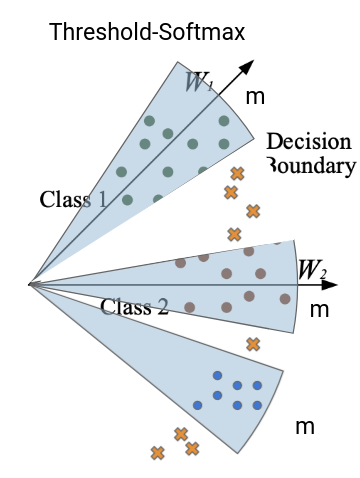
\includegraphics[width=0.25\columnwidth]{50-files/tsm-neg.png}
    \caption{Threshold-softmax with negative samples: crosses are negative samples. We do not know their identities, we just know they do not belong to any of the known identities. Threshold-Softmax naturally uses those samples by placing their identities outside of the known classes decision boundaries, ie, predicting class $\Omega$.}
    \label{fig:neg-tsm}
\end{figure}

\subsection{Experimental study}

We experiment with our new loss function by training on MS1Mv2 and testing on LFW and FGLFW. compare L2-Softmax / Angular Softmax, ArcFace, Threshold-Softmax, Threshold-Softmax with negative samples, at various data availability.

In order to cut training times down, we train on 5\% of the training data for 10 epochs, with a Resnet18 pretrained on ImageNet.

We conduct an experiment with extensive hyperparameter search (for $m$, the learning rate and the weight decay) and sum up our results in Table \ref{tab:tsm-lfw}. In the Threshold-Softmax with negative samples case, we add another 5\% of the dataset with a single negative label. We assess the performance of our proposed loss according to the threshold value in Figure \ref{fig:tsm-angle}.

\begin{table}[]
    \centering
    \begin{tabular}{|c|c|c|}
        \hline
         & LFW & FGLFW \\
        \hline
        L2-Softmax & 97.66 & 88.88 \\
        \hline
        ArcFace & 98.63 & \textbf{95.58} \\
        \hline
        Threshold-Softmax & 98.88 & 93.51 \\
        \hline
        Threshold-SM + Negative & \textbf{98.93} & 95.23 \\
        \hline
    \end{tabular}
    \caption{Accuracy on LFW and FGLFW for various loss functions. Best rejection threshold selected for each method.}
    \label{tab:tsm-lfw}
\end{table}

\begin{figure}
    \centering
    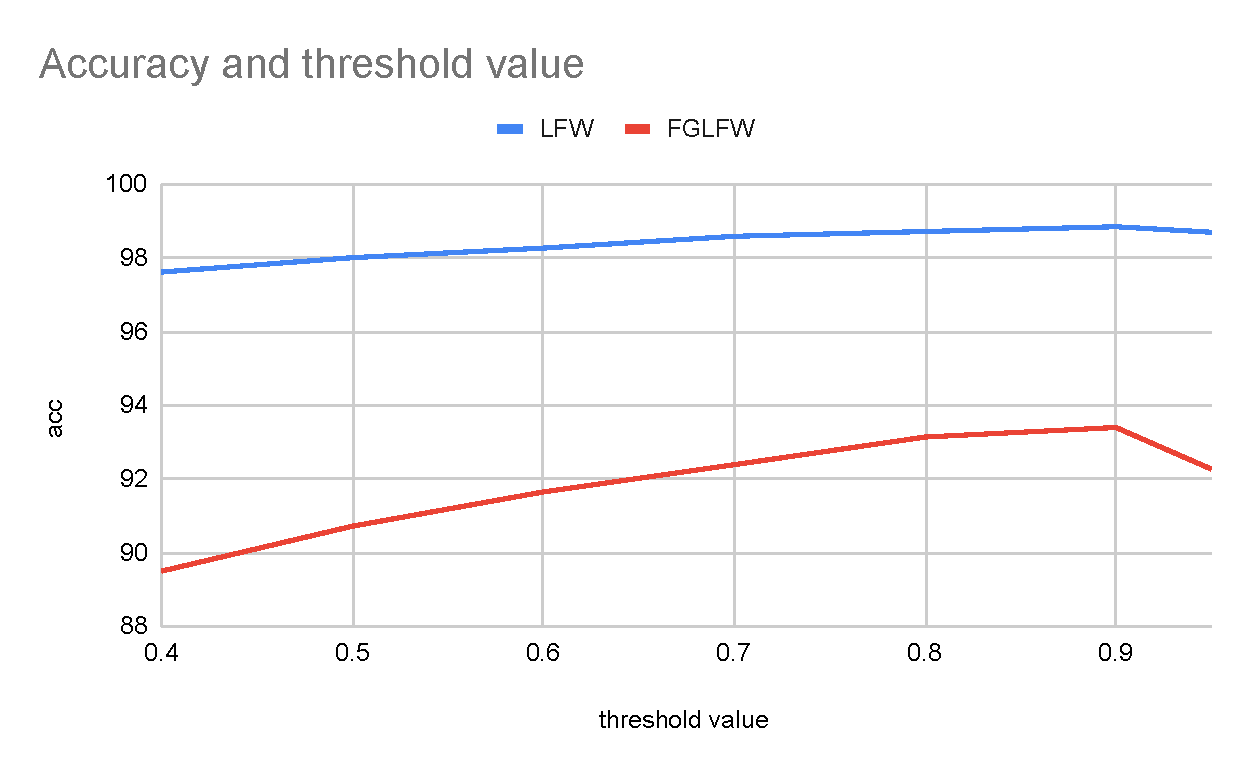
\includegraphics[width=\columnwidth]{50-files/tsm-angle.pdf}
    \caption{Performances on LFW and FGLFW according to the threshold value.}
    \label{fig:tsm-angle}
\end{figure}

We see that the Threshold-Softmax is competitive with ArcFace and better than the raw L2-Softmax. Furthermore, training with negative samples indeed boost the performance of Threshold-Softmax.

Further testing should be conducted with bigger data and epochs budget in order to compare those algorithms in realistic training situations.

It is interesting to note that ArcFace's margin is not mutually exclusive with the cones of trust of Threshold-Softmax and the two could be combined. This is left as future work.

\section{\emph{\arr Contributions}: distractor-robust face recognition for a closed-set of identities}

The following sections will highlight our contributions:

\begin{enumerate}
    \item a comparison of ArcFace and cross-entropy classifiers in the context of closed-set face recognition
    \item a search for a strategy to manually deal with label noise, curate and expend a face recognition dataset for closed-set scenarios
    \item a set of losses and their evaluations allowing to leverage unlabeled negative faces and make face recognition system more robust to distractors. 
\end{enumerate}

\subsection{The limits of metric learning}

Our first attempt of addressing face recognition in our industrial context was based on a publicly available face detection and face recognition pre-trained CNNs. The problem was posed as an open-set face recognition task, and consisted in matching a feature vector extracted from an input photo against each reference image in the database feature vectors, as customary in metric learning. Unfortunately, despite the impressive number, having an accuracy of 99.38\% on LFW means that identifying someone by pair matching among 4000 identities (as we wished initially) triggers 25 positive matches. The performance scored in our setting was substantially worse due to distribution mismatch between the training domain and our application domain.

This shows that the metric learning strategy reached its limits in this setting and is not robust enough to scale to many identities and many distractors. Metric learning aims to learn a powerful embedding function, which is too ambitious for our problem: filtering out distractors, and recognizing a handful of persons of interest. Filtering out distractors better describes the task at hand, allows the net to focus on learning only the facial features for the set of the persons of interest, plus a rejection criterion or margin for rejecting distracting faces.

\begin{figure}
    \centering
    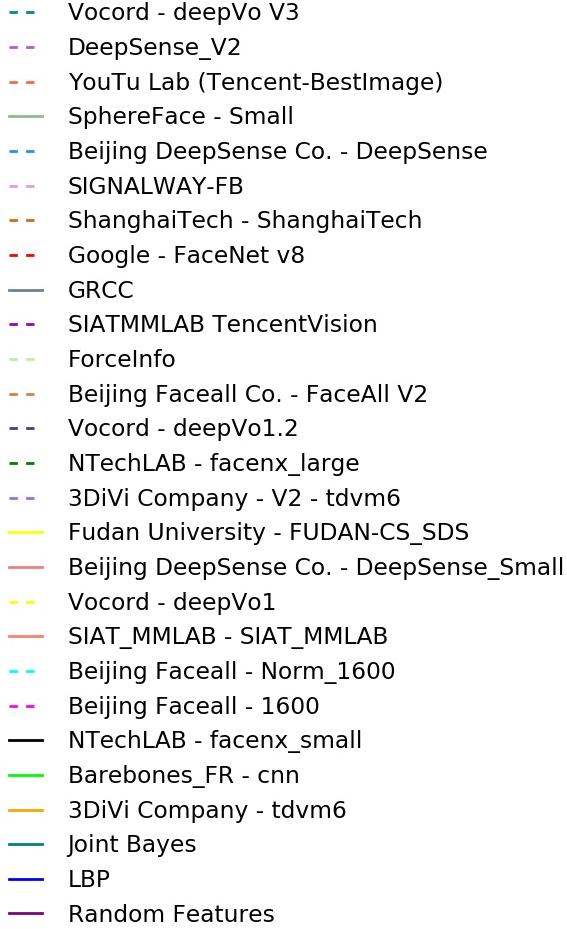
\includegraphics[width=0.3\columnwidth]{50-files/CH1_Legend.png}
    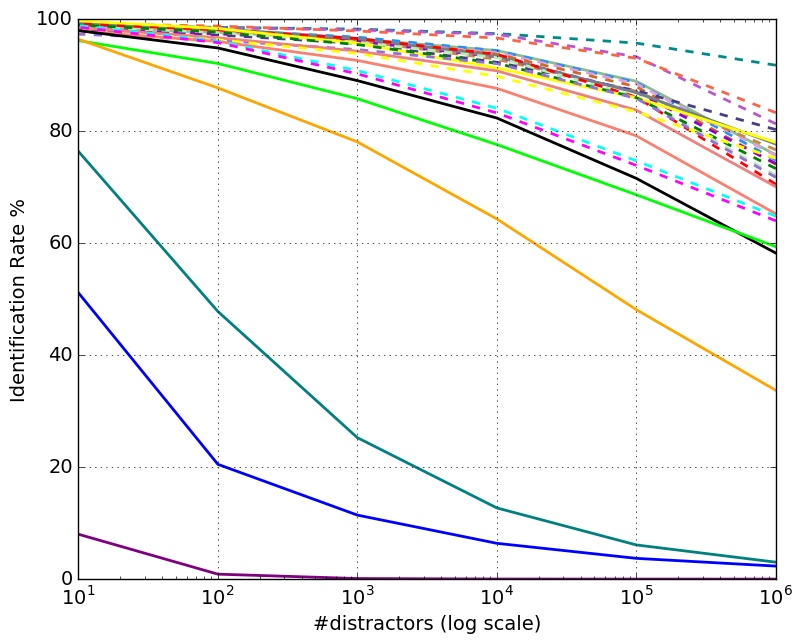
\includegraphics[width=0.45\columnwidth]{50-files/facescrub_rank-1_cmbnd_set_1.jpg}
    \caption{Rank 1 identification performance for contestants on Megaface's Facescrub challenge under various quantities of distractors. Most models have their performance degrading quickly even with 100 distractors only.}
    \label{fig:megafacebad}
\end{figure}

Indeed, Figure \ref{fig:megafacebad} shows that most of the models which participated in the challenge are sensitive to the number of distractors and their performance quickly degrades under 95\%, a threshold under which we consider the models not ready for our application.

\subsection{Back to simple classifiers}

In fact, as the identities to recognize are known ahead of time and part of the training set, it is possible to cast the project as a classification problem, using a regular cross entropy loss. We would be performing the classification from the softmax probabilities, just like the action classification (See \ref{actionclf}).

However, what we miss from such a model is the ability to know when we don't know. This is something modern models are not good at. They tend to be uncalibrated and predict only high confidence scores. \citet{softmaxood} claim that out of domain samples have a lower softmax probability than in distribution samples. This is something we have not observed to be true or sufficient to reliably reject distractors. Moreover, as the nets learn, they tend to overfit the softmax loss and end up predicting higher and higher confidences, even when they're wrong. This makes thresholding the \ac{OoD} rejection confidence score hard as it might change between training runs.

\subsection{Dataset denoising}

We propose a strategy to incrementally clean a dataset from label noise by expending the set of identities to recognize. We explicitly train on negative samples ("distractors") and select a subset of HFaces' identities as a positive training set and the rest as negative set. This allows to grow the positive set in a controlled way, so that the negative set can be denoised progressively. If we had to investigate a classifier among thousands of identities at once, it would be extremely hard to gain insight into the dataset and take actions. Instead, we use as a positive set the top N most popular identities, learn a model, evaluate it, clean or complete the training set, then add another N positive identities when the performances are good for our setting, and iterate.

\subsection{Precision / Recall for dataset construction}

\subsubsection{Motivation}

As the training data can be modified as well in order to address the task, several questions have to be answered in order to grow the dataset in a principled way. Mainly, at any point in time, there are 3 possible situations and their associated response:
\begin{enumerate}
    \item Everything works well enough: grow the set of VIPs
    \item Some VIPs seem to cause too much confusion and trigger too many false positives: rework the data for those identities (looking for errors, low quality or confusing samples) in order to identify harmful samples
    \item Some VIPs are not detected in tests : add samples. Those identities have insufficient data to generalize correctly.
\end{enumerate}

Which one of those actions to take is crucial in order to control the growth of the model and its performance.

\subsubsection{Principles}

\begin{figure}
    \centering
    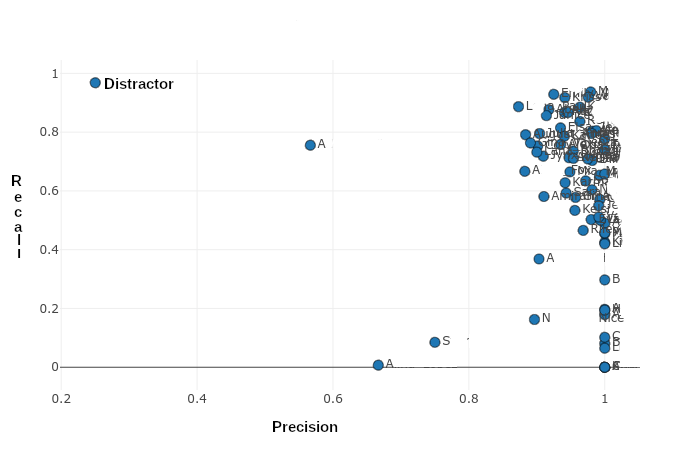
\includegraphics[width=\columnwidth]{50-files/pr-plot.png}
    \caption{Each class (abbreviated to the first letter of the nperson's ame) is placed on this grid depending on its precision and recall scores. Top right is best, bottom left is worst. We aim to find strategies that help moving each point right and up.}
    \label{fig:pr-plot}
\end{figure}


Diagnosing the current state of the dataset in order to choose what to do next happens to be easy thanks to simple metrics. By computing precision / recall by class we get a view of the model performance. In order to easily visualize which class need work, we plot each class on a grid, seen in Figure \ref{fig:pr-plot}. We empirically hypothesize that classes with low precision suffer from noisy training data and/or labels, while classes with low recall indicate a lack of training data.

These assumptions brings insight into the model's state, is easy to implement, interpret and use but bears the drawback that some additional effort must be taken in order to build a meaningful test set for each identity. As we observe strong outliers on the precision/recall plots while building the dataset, we hypothesize that the performance across identities is not correlated (or not enough), and therefore we believe we cannot use a random subset of identities to estimate the overall performance.

In our situation, we accept trading recall for precision as false positives damage the user experience with erroneous suggestions or search results. With false negatives, no labeling is performed, and the user browsing is not impacted.

\subsubsection{Results}

In order to investigate these hypotheses, we select a class which performs well in both precision and recall and run three experiments:

\begin{enumerate}
    \item A base run gives 94\% precision and 99\% recall.
    \item We subtract 50\% of the training data for that class, obtaining 98\% precision and 86\% recall. Here, it is clear that removing data deteriorates recall. By reducing the amount of training data, the identity is more narrowly represented, thus less sensible to accept other faces as belonging to it: the precision slightly increases.
    \item We introduce label noise by integrating someone else's samples into this class' training data. We obtain 94\% precision and 98\% recall.
\end{enumerate}

This data point seem to suggest that recall indeed correlates with the amount of data for a class. Unfortunately, precision does not negatively correlate with label noise. The classifier seems to overfit the noise rather quickly and learn a multimodal class. The question of detecting noisy classes remains unanswered by this approach.

\subsection{Experiments}

\begin{figure}
    \centering
    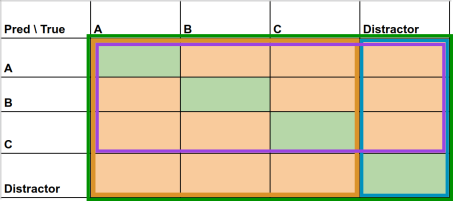
\includegraphics[width=0.6\columnwidth]{50-files/cm.png}
    \caption{We compute some metrics by selecting various meaningful subsets from the confusion matrix: \textcolor{blue}{distractor accuracy} (blue), \textcolor{orange}{identification accuracy} (orange), \textcolor{violet}{kept accuracy} (violet), and \textcolor{ForestGreen}{total accuracy} (green). For each subset, the metric is computed as the sum of the green cells it contains divided by the sum of all cells it contains. A, B, and C are three fictitious identities for illustration purposes}
    \label{fig:cm-metrics}
\end{figure}

We devise a set of experiments in order to evaluate the progress done on the task of face recognition on HFaces. For each experiment, we measure:
\begin{itemize}
    \item the accuracy on the distractor set: among all distractors how many have been predicted as such, ie, the true rejection rate (See Figure \ref{fig:cm-metrics}).
    \item the identification accuracy: the recognition accuracy among non-distractors (See Figure \ref{fig:cm-metrics}).
    \item the overall accuracy on all test samples (See Figure \ref{fig:cm-metrics}).
    \item the mean of the F1 score of each class
    \item the accuracy of kept (non rejected) predictions. We consider that we reject predictions classified as distractors (See Figure \ref{fig:cm-metrics}). This allows us to evaluate how many false identification will be performed on the platform, and choose our precision / recall tradeoff. 
    \item When techniques give scores with predictions and the model performs reasonably well, wrong predictions are given a lower score and correct prediction a higher score. This allows us to trade precision for recall, as we can find a threshold which rejects predictions with low scores until a chosen true positive ratio. Thus, we also compute the identification and total accuracy for 95\% and 99\% true positives, giving us an estimate of the recall for both test sets at those true positive rate goals.
\end{itemize}

We emphasize the industrial context: this tool is to be used in order to label videos on the customer's platform. As such, it is better not to annotate a video than predict a wrong label. Setting a false acceptance rate of 5\% / 1\% (ie 5\% / 1\% of wrong predicted labels, a precision of 95\% / 99\%), we evaluate the recall by computing the accuracy on the identification set and the entire test set. Results are summarized in Figure \ref{fig:tpr}.

We compare several models: ArcFace, and cross-entropy classifiers. We train a simple classifier (CE) also explore several techniques for exploiting distractors from the training set, and rejecting them at inference:  an extra class for distractors (DCE), maximizing entropy on distractors (ME), minimizing logits on distractors (ZLog). We report, in Table \ref{tab:frmetrics}, the various metrics \emph{at the maximum accuracy}.

\begin{figure}
    \centering
    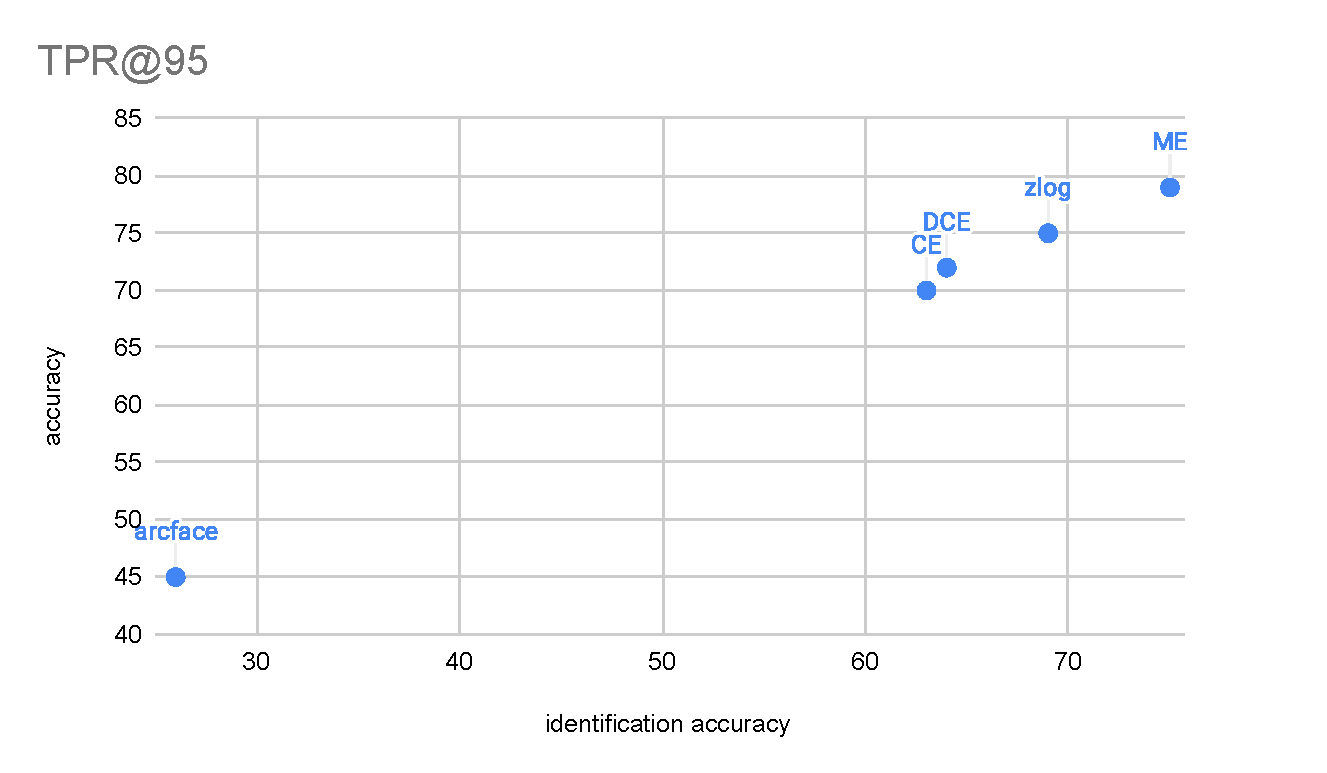
\includegraphics[width=\columnwidth]{50-files/TPR@95.pdf}
    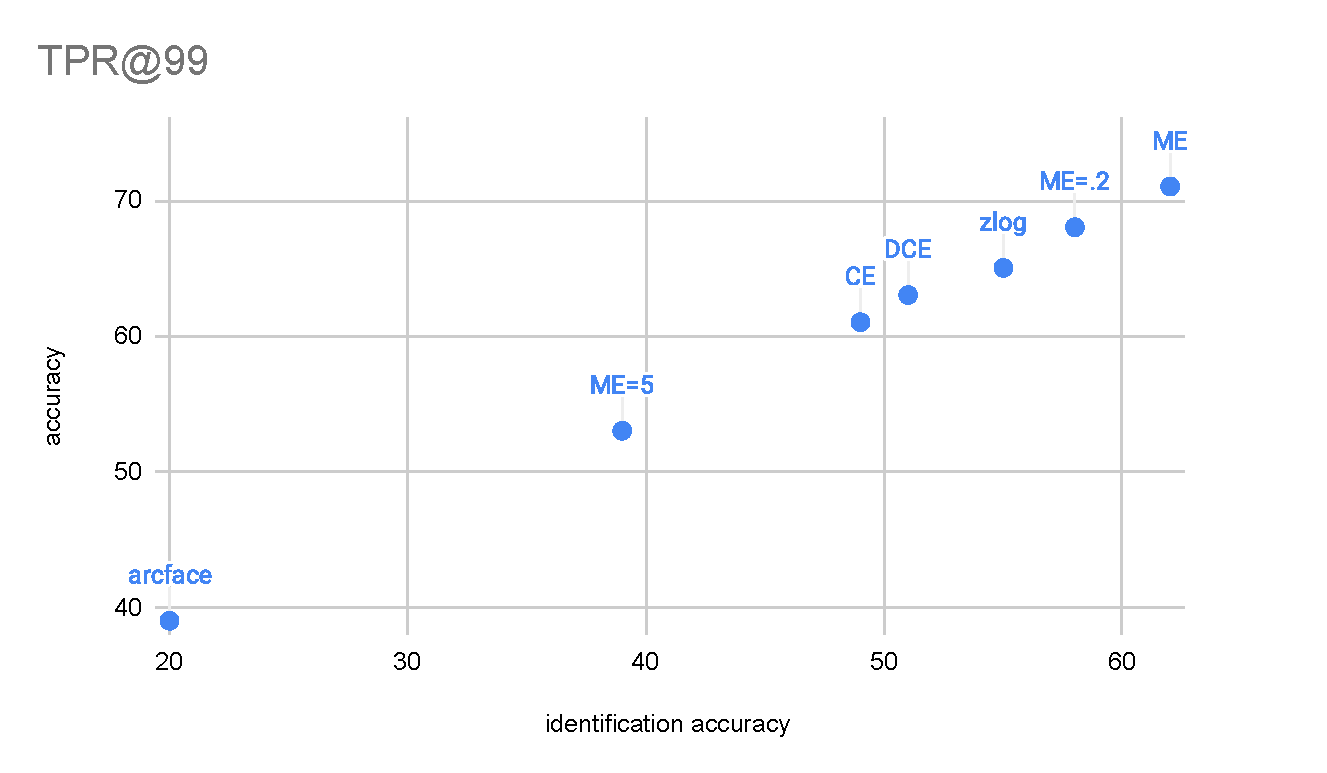
\includegraphics[width=\columnwidth]{50-files/TPR@99.pdf}
    \caption{Identification accuracy and total accuracy for a true acceptance rate of 95\% / 99\%. CE: Cross-Entropy, DCE: Cross-Entropy+Distractors, ME=$x$: Cross-Entropy+MaximumEntropy with maximum entropy weight $x$, zlog=Zero-Logits.}

    \label{fig:tpr}
\end{figure}

\begin{table}[]
    \centering
    \begin{tabular}{|l|c|c|c|c|c|}
    \hline
        Model & distractor     & identification   & total           & mean F1       & kept \\
              & accuracy       &   accuracy       & accuracy        &               & accuracy \\
        \hline
        \hline
        ArcFace & 78.38        & 43.93            & 52.03           & 0.40          & 73.11 \\
        \hline
        CE   & 79.65           & 73.51            & 74.96           & 0.65          & 85.4 \\
        \hline
        DCE & \textbf{95.17}   & 65.35            & 72.36           & 0.62          & \textbf{92.82} \\
        \hline
        ZLog & 79.09          & \emph{78.67}      & \emph{78.77}    & \emph{0.66}   & 84.92 \\
        \hline
        ME & \emph{89.56}     & \textbf{78.93}    & \textbf{81.43}  & \textbf{0.72} & \emph{91.05} \\
        \hline
    \end{tabular}
    \caption{Various metrics for each model, selected at maximal accuracy. CE: Cross-entropy, DCE: Cross-Entropy+Distractors, ME: Cross-Entropy+MaximumEntropy with maximum entropy, ZLog=Zero-Logits. \textbf{Best} and \emph{second best} results are highlighted}
    \label{tab:frmetrics}
\end{table}


\subsubsection{ArcFace}

\begin{figure}
    \centering
    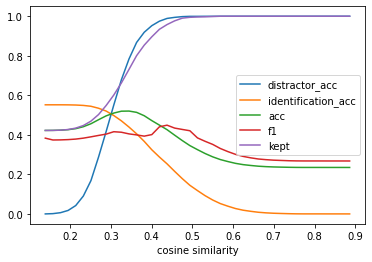
\includegraphics[width=0.45\columnwidth]{50-files/arcface-all.png}
    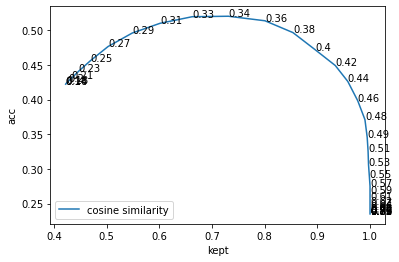
\includegraphics[width=0.45\columnwidth]{50-files/arcface-acc-kept.png}
    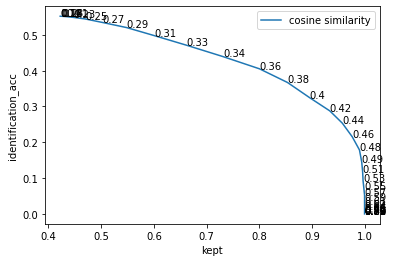
\includegraphics[width=0.45\columnwidth]{50-files/arcface-id-kept.png}
    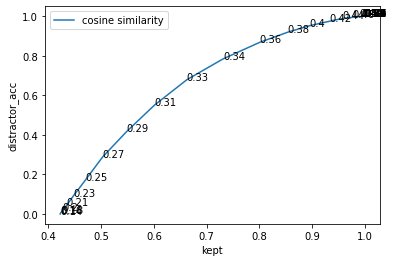
\includegraphics[width=0.45\columnwidth]{50-files/arcface-distr-kept.png}
    \caption{a) Various metrics for the ArcFace model as predictions are set as distractors under various cosine similarity values. b,c,d) As we sweep over the threshold cosine similarity value and reject more samples as distractors, we look at the variations on the metrics against the kept accuracy.}
    \label{fig:arcface-plots}
\end{figure}

We first verify our claim that metric learning is not robust in our setting. We reuse the pretrained ArcFace model published by \url{https://github.com/foamliu/InsightFace-v2}. The important things to note are:

\begin{itemize}
    \item this model has been trained for a face-independent protocol, that is, it has not been trained on the people it was meant to recognize;
    \item this model has several data biases: our distribution includes more females than males, very few above the age of 50. The training set is broader than this narrower distribution of ours. The model is faced with a narrower and more fine-grained task than intended;
    \item Metric learning makes it hard to know when we don't know, thus rejecting distractors is not easy;
    \item ArcFace protocol is about computing the cosine similarity between the representation of the input image and a reference image. For identification, we randomly choose one reference image per class. The choice of that reference image could have been selected against a validation set for minor gains. We made sure that the different metrics do not dramatically change between each run.
    \item We set a distractor threshold. If all reference images have a cosine similarity lower than this threshold, we reject this input as a distractor. We compute our metrics sweeping over threshold values, shown in Figure \ref{fig:arcface-plots}.
\end{itemize}


We get a best accuracy value of 52.3\% for a distractor accuracy of 78\%, an identification accuracy of 44\% and F1 score of 0.40.

\subsubsection{Cross-Entropy (CE)}

\begin{figure}
    \centering
    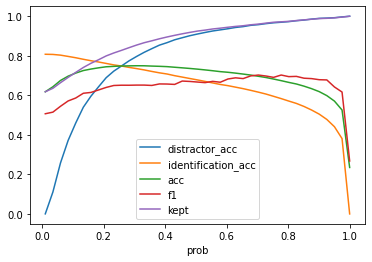
\includegraphics[width=0.45\columnwidth]{50-files/ce-all.png}
    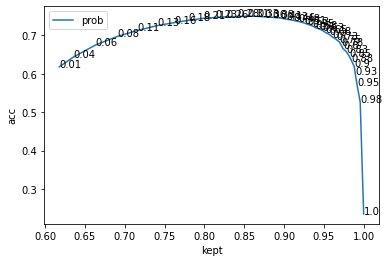
\includegraphics[width=0.45\columnwidth]{50-files/ce-acc-kept.png}
    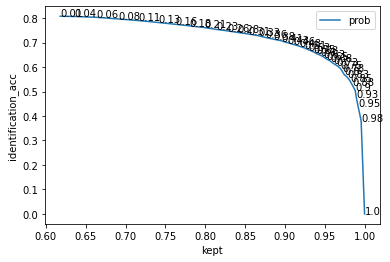
\includegraphics[width=0.45\columnwidth]{50-files/ce-id-kept.png}
    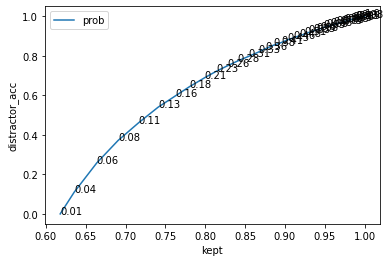
\includegraphics[width=0.45\columnwidth]{50-files/ce-distr-kept.png}
    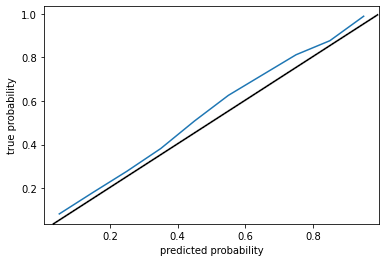
\includegraphics[width=0.45\columnwidth]{50-files/ce-calibration.png}
    \caption{Various metrics for the CE model as predictions are set as distractors under various probability values. Last plot is the network's calibration.}
    \label{fig:ce-plots}
\end{figure}

We now compare the advanced ArcFace loss with a naive softmax+cross entropy loss, trained on the persons of interest only. This model has no built-in way of signaling distractors. We are going to assume that the distractors produce predictions with lower confidence, and threshold on low confidence scores.

Figure \ref{fig:ce-plots} indicates that this heuristic holds some truth. It seems that around 90\% of distractors have a confidence score below 0.25 and half of the people of interest get a confidence score over 0.95. Unfortunately this heuristic is not entirely satisfying. As the rejection threshold increases, the overall accuracy slowly decreases.

It is unsurprising that the base identification accuracy of 81\% is much greater than the 55\% of ArcFace. This model gets a peak accuracy of 75\%, for a distractor accuracy of 80\%, an identification accuracy of 73\%, and a F1 score of 0.65. This model is already indisputably more suited for our task.

\subsubsection{Cross-Entropy with Distractors (DCE)}

\begin{figure}
    \centering
    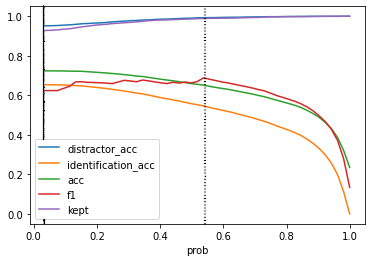
\includegraphics[width=0.45\columnwidth]{50-files/dce-all.png}
    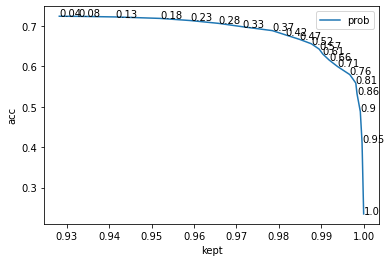
\includegraphics[width=0.45\columnwidth]{50-files/dce-acc-kept.png}
    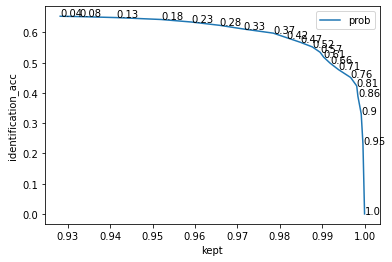
\includegraphics[width=0.45\columnwidth]{50-files/dce-id-kept.png}
    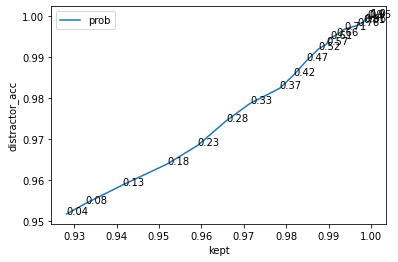
\includegraphics[width=0.45\columnwidth]{50-files/dce-distr-kept.png}
    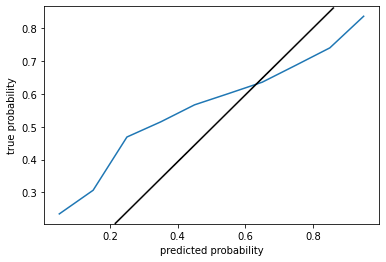
\includegraphics[width=0.45\columnwidth]{50-files/dce-calibration.png}
    \caption{Various metrics for the DCE model as predictions are set as Distractors under various probability values.}
    \label{fig:dce-plots}
\end{figure}


Aiming to improve both the representational power of our model and teaching it the ability to reject distractors, we add distracting faces to our training data that have to be classified as their own distractor class. Similarly to the previous model, we evaluate how the different metrics behave when we also consider as distractors predictions below a given threshold in Figure \ref{fig:dce-plots}. The peak accuracy of 72\% is below the one of the simple classifier, explained by a lower ability to recognize the people of interest (from 73\% to 65\%) but a much greater ability to detect distractors (from 80\% to 95\%). Overall the models have a comparable F1 score of 0.62. However, the model behaves better in our industrial scenario, as shown in Figure \ref{fig:tpr}.

\subsubsection{Cross-Entropy + ZeroLogits (zlog)}

\begin{figure}
    \centering
    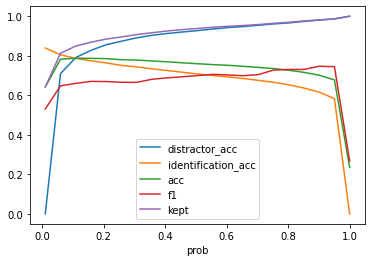
\includegraphics[width=0.45\columnwidth]{50-files/zlog-all.png}
    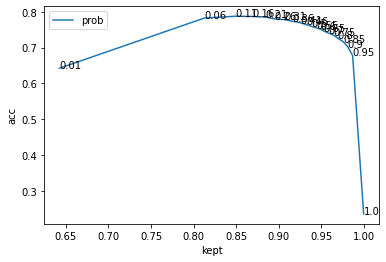
\includegraphics[width=0.45\columnwidth]{50-files/zlog-acc-kept.png}
    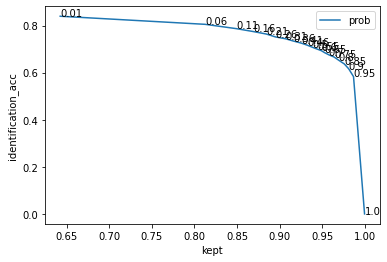
\includegraphics[width=0.45\columnwidth]{50-files/zlog-id-kept.png}
    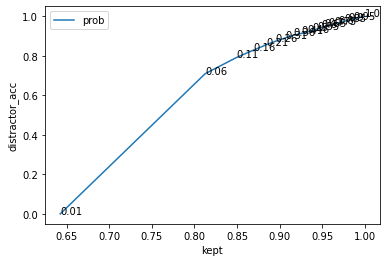
\includegraphics[width=0.45\columnwidth]{50-files/zlog-distr-kept.png}
    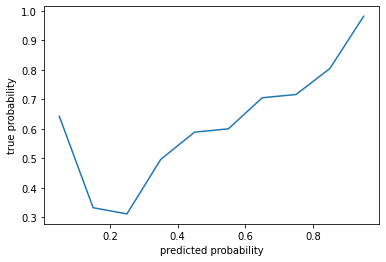
\includegraphics[width=0.45\columnwidth]{50-files/zlog-calibration.png}
    \caption{Various metrics for the zlog model as predictions are set as Distractors under various probability values.}
    \label{fig:zlog-plots}
\end{figure}

Inspired by \citet{goodosr}, we hypothesize that distractors can be sorted by a lower logit value than persons of interest. Distractors are not their own class anymore, but are discriminated from the low logits they produce. We propose penalize their square logits, further encouraging them to zero, and classify only the persons of interest with a cross-entropy loss.

We find that this brings some improvements in identification accuracy and total accuracy, bringing the F1 score to 0.66. This model also performs better when fixing the true positive rate.

However, contrarily to \citet{goodosr} we don't observe logits to be more informative than softmax probabilities. We tried thresholding distractors with logits in each model, every time bringing equivalent or lower results. For this reason, we do not report those results.

\subsubsection{Cross-Entropy + Maximum Entropy (ME)}

\begin{figure}
    \centering
    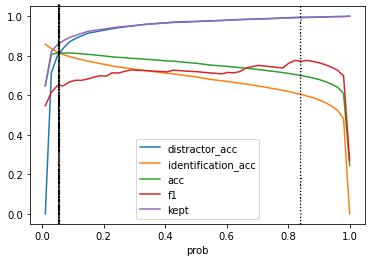
\includegraphics[width=0.45\columnwidth]{50-files/me-all.png}
    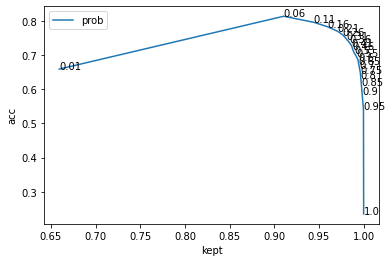
\includegraphics[width=0.45\columnwidth]{50-files/me-acc-kept.png}
    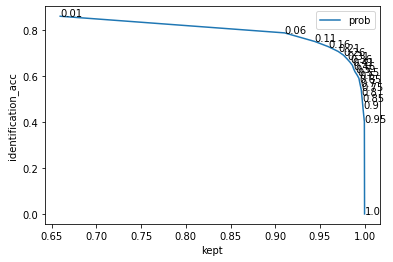
\includegraphics[width=0.45\columnwidth]{50-files/me-id-kept.png}
    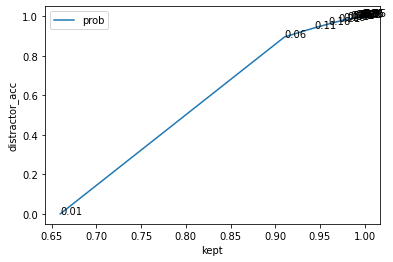
\includegraphics[width=0.45\columnwidth]{50-files/me-distr-kept.png}
    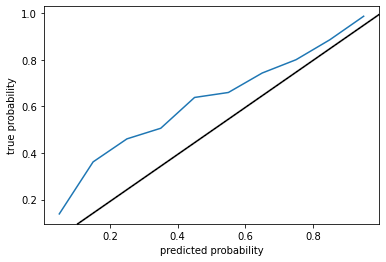
\includegraphics[width=0.45\columnwidth]{50-files/me-calibration.png}
    \caption{Various metrics for the ME model as predictions are set as distractors under various probability values.}
    \label{fig:me-plots}
\end{figure}

Finally, observing that the zlog model was not working as well on logits than on probabilities, despite the loss working directly with them, we envision working on probabilities. Model CE shows that distractors naturally produce lower probabilities, so we aim to predict a maximum entropy (flat) distribution for distractors.

We evaluate this model with weights 1, 5, 0.2 on the maximum entropy loss. A weight of 1 brings the best results, shown in Figure \ref{fig:me-plots}.

\subsubsection{Discussion}

Overall, the ME approach results in the best way to leverage distractors in order to build our industrial system, as can be seen on the TPR plots. It results in the best total and identification accuracy and F1, while being the runner up in kept accuracy. The ZLog technique scores second but is inferior in every way.

The DCE method attracts our attention as well, scoring the highest distractor accuracy and kept accuracy. However, its identification and total accuracy, as well as its F1 are the lowest among the cross-entropy classifier. We conclude that this strategy just over emphasizes classifying as distractor, decreasing identification recall too strongly. Being only 1\% lower in kept accuracy, the ME is a better compromise as we will have a slightly higher error \emph{ratio} but predict a much higher \emph{number} of correct predictions.

\section{Conclusion}

We showed that off-the-shelf  face recognition classifiers, trained with ArcFace, were not satisfying for our industrial scenario. We first explored remaining in the Metric Learning realm and proposed the Threshold-Softmax loss function that is able to use negative samples that are cheaper to collect. However, Threshold-Softmax remains a technique for subject-independent face verification and indentification.

We moved away from metric learning and went back to classifier as our system only has to recognize identities known ahead of time, in a subject-dependent, open-set fashion. We explored various ways of making it robust to distractors, unknown people that the system must learn to discriminate. We explored various techniques to reject distractors at inference time and use distractors at training time, and found that maximizing the entropy for distractors to be the best performing strategy we tried. It is used in production today.

We search for a principled way to refine and extend the training set, leveraging precision/recall plots. While our hypothesis on recall looks promising, we still don't know how to manipulate precision and our hypothesis has been disproved.

The final system is currently used in production, labeling 15k videos a day, and the extracted labels are used as planned to enrich the user experience.

% FIXME grouper par figure plutôt qu'xp
\chapter{Fixing Datasets with generative models}
\label{chap:gan}

\newcommand{\pdata}[0]{\p_\texttt{data}}
\newcommand{\pfake}[0]{\p_\texttt{fake}}
\newcommand{\ppath}[0]{\p_\texttt{path}}
\newcommand{\pz}[0]{\p_z(z)}

\section{Introduction}

Deep Learning has proven to be successful at generating natural images. \citet{dagan} see in this ability an opportunity to improve datasets by generating more data and shows performance improvements in classifiers when using generated data as a supplement to the training data.

Using generative models in the context of face recognition is appealing. Many pictures per identities are needed in order to teach a classifier that it should be invariant to lighting, pose, makeup, haircuts, etc. However, as we grow the number of identities that the system has to recognize, there is a risk that the classifier does not learn the invariants for identities with less variations in training data. In other words, we fear that the classifier learns useful features only for the identities with many diverse pictures and overfit the case with little training data.

Generating data gives us the opportunity to create the diversity of pose, lightning etc for the identities with the least diverse identities.

In this chapter we lay out a review of the different techniques of generative models we explored before settling on one. We will explore \acp{GAN} and \acp{VAE}, and more specifically the \ac{VQVAE} for which we will present our contribution: an expiration process for the codebook in order to improve its training dynamics and performance. We then introduce our chosen system for data augmentation in the context of face recognition.

\section{Generative models for building invariants}

In our dataset, some people were always facing the camera, or never smiling, while others exhibited larger variations in pose, exposition or image quality. We hypothesized that this could lead the classifier to learn some shortcuts like "This is not Person \textbf{A} because that person is smiling, \textbf{A} never does". One obvious way to teach invariants to classifier is to feed them proper data exhibiting those invariants. In face recognition, that would translate in making sure that all identities have various level of illuminations and a wide variety of poses so that the classifier does not learn shortcuts. We aim to complement the dataset with the missing variations of each identity by training a generative model. Hopefully, the model would learn the general concepts of face geometry, disentangle it from facial identity, and could reenact anyone's face into any pose.

\section{Problem definition}

Let $\mathcal{D}$ be a dataset containing some face pictures $x_i$ and their identity label $y_i$ such that $(x_i, y_i) \in\mathcal{D}$. Let $p_i \in \mathcal{P}$ be an unknown semantic latent vector representing pose, lighting etc, containing no information about $y_i$, such that a powerful generative model $G$ could hold $G(y_i, p_i) = x_i$ (see figure \ref{fig:G_specs}).

Those faces can be considered samples of an underlying "face photo" manifold with dimensions describing semantic variations such a lighting, pose or identity. We would like to learn a generator $G(y_i, z), z \sim \pz$. $G$ learns to interpret $z$ as a $p_i$ and decode it as a pose / illumination / etc vector that doesn't include any identity information. Ideally, $z$ is a probability distribution that is easy to sample from (eg standard normal). We could then reenact any identity $y$ by sampling $z$ vectors at will.

\begin{figure}[ht]
    \centering
    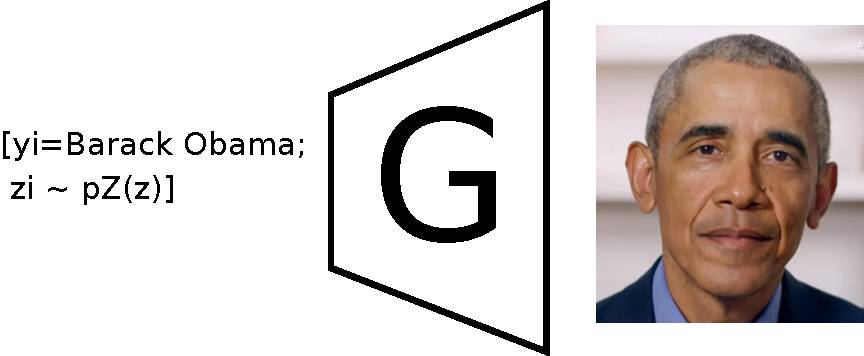
\includegraphics[scale=0.5]{60-files/GANVAE-1-1}
    \caption{$G$ is a generator that turns a person identitifier $y_i$ and a latent variable $z_i$ into an image.}
    \label{fig:G_specs}
\end{figure}

\section{Generative Models}
\subsection{Fundamentals}
When trying to generate data, we wish to model $\p(X)$ for any data distribution $X$ in terms of its individual components. For instance, for image data, we learn to model images $x \in \mathcal{X}$ by modeling the color probability distribution of each of its pixels $x_{1..H, 1..W}$, by assuming independence.

\begin{equation}
\label{gen_model1}
    \p(X=x) = \prod_{i=1}^H \prod_{j=1}^W \p(X_{i, j}=x_{i, j})
\end{equation}

With such a simple model, $\p(X_{i, j})$ is left as an arbitrarily sophisticated or simple distribution of our choice, such as a categorical distribution over discretized pixels values (with parameters $\theta_{i,j}$)

\begin{equation}
    \p(X_{i,j}) = \texttt{Cat}(X_{i,j}; \theta_{i,j})
\end{equation}

or Gaussian distributions over values (with mean parameters $\mu_{i,j}$ and standard deviation parameters $\sigma_{i,j}$)

\begin{equation}
    \p(X_{i,j}) = \mathcal{N}(X_{i,j}; \mu_{i,j}, \sigma_{i,j})    
\end{equation}


Once the individual pixel probabilities parameters (ie $\theta_{i,j}$ or $\mu_{i,j}, \sigma_{i, j}$) have been estimated from data, one could sample a value for each pixel and get an image.

However, this modeling is trivial and would produce pictures that looks nothing like real images because it considers each pixel as independent and does not take into account patterns and spatial correlations. 

\subsection{Auto-regressive models}

This components independence assumption leads to very poor results, especially in image generation. Instead of sampling each component independently, we could sample each component one after another, in any predefined order, based on some of the previously sampled values. In which case $\p(X_{i,j})$ becomes a distribution conditioned on the previous $k$ components. The graphical model is illustrated in figure \ref{fig:autoreg-chain}.

For image data, those individual components are pixels, and a full image is sampled pixel by pixel. Each sampling operation operates on a context window constituted of the previous samplings. As we consider bigger context windows $k$, the models needed become more complex and bigger and that is when Deep Learning comes into play. This image is progressively sampled following an ordered set of pixel coordinates $\Psi$ (usually left to right and top to bottom, but not limited to).

\begin{equation}
    \p(X) = \prod_{i = 0}^{|\Psi|} \p(X_{\Psi_i} | x_{\Psi_{i-1}}, .., x_{\Psi_{i-k}})
\end{equation}

This is the approach coined by PixelCNN \citep{pixelcnn}, PixelRNN \citep{pixelrnn}, PixelCNN++ \citep{pixelcnn++} or PixelSNAIL \citep{pixelsnail}. At inference time, we sample pixels one by one, each requiring a model forward pass. This exhibits the major drawback of auto-regressive models for image synthesis: they require $H \times W$ forward passes, making it extremely slow and computationally intensive. Moreover, as the images grow bigger, not only more forward passes are needed, bigger models are needed as well in order to grow their receptive fields and context windows accordingly. A single pass of PixelCNN is shown in figure \ref{fig:pixelcnn}.

\begin{figure}[ht]
    \centering
    \includegraphics[scale=0.5]{60-files/chain-pixelcnn.pdf}
    \caption{Conditional probability graph of an autoregressive model. Each pixel depends on the previous ones, iteratively.}
    \label{fig:autoreg-chain}
\end{figure}

\begin{figure}[ht]
    \centering
    \includegraphics[scale=0.8]{60-files/pixelcnn.png}
    \caption{A PixelCNN sampling a pixel value for the current pixel from its surrounding context. White pixels are still undetermined grey pixels have already been sampled. Shown in red is the softmax output describing the probability distribution of the current pixel values conditioned on the context window. Image from \citet{pixelcnn}}
    \label{fig:pixelcnn}
\end{figure}

Modern auto-regressive models such as the \ac{VQVAE} \citep{vqvae} or \ac{VQGAN} \citep{vqgan} try working around this complexity by only sampling small pictures or small representations, leaving the actual high quality rendering to another method, such as convolutional upsamplers, convolutional decoders, or \acp{GAN}. The \ac{VQVAE} will be described in section \ref{section:vqvae}.

\section{Latent-Variable Models and Variational AutoEncoders}
\label{sec:vae}
\subsection{Principles}

\begin{figure}[ht]
    \centering
    \includegraphics[scale=0.5]{60-files/chain-vae.pdf}
    \caption{Conditional probability graph of a Latent Variable Model (LVM). The whole image $x$ is sampled at once from a lower dimensional encoding $z$.}
    \label{fig:vae-chain}
\end{figure}

Instead of having a long chain of random variable dependency (ie the previous components), we can assume that there is a lower dimensional explicative random variable $z \sim \pz$, and that a powerful function could decode from it all the components at once (compare figure \ref{fig:autoreg-chain} and \ref{fig:vae-chain}). For images, this embodies the idea that the pixels of an image can be reduced to a much denser amount of semantic information such as "a child sitting on a bench and eating ice cream in a park" or a low dimensional feature vector. We can thus model the data probability density as the probability of a data point $x$ decoded by all possible codes $z$:

%FIXME: petit p? petit x? petit q?

\begin{equation}
    \p(x) = \int \p(x | z)\pz dz = \int \pz \prod_{i=1}^H \prod_{j=1}^W \p(x_{i,j} | z) dz
\end{equation}

\begin{equation}
\label{eq:logppx}
    - \log \p(x) = - \log \int \p(x | z) \pz dz
\end{equation}

In our case, this code $z$ is considered unknown and has to be discovered by the training procedure as well. We often chose $z$ to be a continuous feature vector and $\pz$ to be a standard Gaussian as it is easy to sample from. $\p(X | Z)$, called "decoder", generates the data components from the code. It usually is a neural network suited for the data type.

The integral in Eq \ref{eq:logppx} can be rewritten as an expectation: 

\begin{equation}
    - \log \p(x) ~= - \log \IE_{z \sim \pz}[\p(x| z)]
\end{equation}

The expectation outside the $\log$ is unfortunate: the log of the expected value would need many samples in order to be accurate, and all those probability multiplications would be numerically unstable.

Thankfully, Jensen's inequality gives us a useful lower bound: $f(\IE[x]) \leq \IE[f(x)]$ for any convex function $f$. So, the $\log$ can be moved inside the expectation at the cost of a lower bound.

\begin{equation}
    - \log \p(x) \leq \IE_{z \sim \pz} [- \log  \p(x | z) ]
\end{equation}

Learning this model with Maximum Likelihood Estimate for large datasets is impractical as we would first need to sample a $z$, find a sample in the dataset that is best explained by the decoder for that $z$, and perform the MLE step.

The VAE \citep{vae} proposes to solve this with more neural networks. The simple fix is to learn an "encoder" $q$ that learns which $z = q(x)$ explains $x$ the best. We can then take a training sample, encode it to a $z$, decode it back, and optimize for reconstruction and penalize the log probability of $z$ according to the prior $\pz$ as well.

This, however, would not make a good generative model as there is no incentive that the encoder covers the whole volume of $\pz$. Instead of encoding $z = q(z|x)$ as a deterministic mapping, $q(z|x)$ can be turned into probability density parameters from which we can sample $z$. We can thus read $z \sim q(z|x)$, and instead of penalizing the log probability of $\pz$, we penalize the Kullback-Liebler divergence $D_{KL}(q(z|x) || \pz)$. The KL divergence measures the dissimilarity between two probability distributions. With $q$ being pushed to resemble the prior, we hope to enforce full utilization of the prior probability space.

Formally, if we use this surrogate distribution $q(z|x)$ to ease smart sampling from $\pz$, we are doing \emph{importance sampling}, and get $\IE_{z \sim \pz} [\p(x|z)] = \IE_{z \sim q(z|x)}[\frac{\pz}{q(z|x)}\p(x|z)]$. Taking the log and applying Jensen's inequality, we obtain

\begin{equation}
\begin{split}
    - \log \p(x) & = - \log \IE_{z \sim \pz} [\p(x | z) ] \\
    & = - \log \IE_{z \sim q(z|x)} [ \p(x | z) \frac{\pz}{q(z|x)} ] \\
    & \leq \IE_{z \sim q(z|x)} [- \log \p(x | z)  - \log \frac{\pz}{q(z|x)}] \\
    & \leq -\IE_{z \sim q(z|x)}[\log \p(x | z)] + \IE_{z \sim q(z|x)} [- \log \frac{\pz}{q(z|x)}] \\
\end{split}
\end{equation}

This formalizes the \ac{ELBO}:

\begin{equation}
    - \log \p(x) \leq ELBO(x) = - \IE_{z \sim q(z | x)} \log \p(x | z) - D_{KL}(q(z | x) || \pz)
\end{equation}

We usually interpret this loss as two terms that must be minimized: a reconstruction term and a prior divergence term. We aim to learn an encoder that produces representations whose distribution is similar to an isotropic gaussian, and a decoder that is able to decode any sample from the $\mathcal{N}(0, \mathbf{I})$ prior into a realistic data sample.  While this helps this intuitive explanation is the source of some misconceptions that are beyond the scope of this document.

\subsubsection{The reparameterization trick}

It is important to note that sampling is a discrete operation. As $z$ is sampled from $q$, it is not natural to learn both $q(z|x)$ by backpropagation. In order to be able to backpropagate into $q$ we have to make it a differentiable operation.

In order to do so we model $q$ as an isotropic Gaussian of D dimensions. We make the neural network modeling $q$ output two sets of values: $\boldsymbol{\mu}(z|x)$ and $\boldsymbol{\sigma}(z|x)$, ie the mean and standard deviation of each dimension of the Gaussian. We observe that sampling from $\mathcal{N}(\boldsymbol{\mu}(z|x), \boldsymbol{\sigma}(z|x))$ is the same as sampling from $\boldsymbol{\mu}(z|x) + \boldsymbol{\sigma}(z|x)\mathcal{N}(0, \mathbf{I})$. Elementwise addition and multiplication are differentiable, therefore this form allows to backpropagate into $q$. This is known as the reparameterization trick.


\subsection{Limits}

It is to be noted that the shortcomings of the VAE are well known:

\begin{enumerate}
    \item The KL term and sampling operation prevents the decoder from having an accurate latent variable to decode. Thus, the produced samples are notoriously blurry.
    
    \item The reconstruction term and divergence term balance in counter-intuitive ways. The ultimate VAE goal is not to learn a meaningful latent vector but to assign the correct probability density to the data distribution. When possible, the encoder ignores the input sample, produces exactly the prior distribution (turning the KL term to zero), and decodes samples at random. This is to be expected, especially when powerful decoders are used.
\end{enumerate}



\subsection{Information Bottleneck}

\subsubsection{General concept}

The reparameterization trick and the KL term in order to fit a noise distribution lead to the variational information bottleneck, used as a layer. Through this layer, only the information necessary for minimizing the task's loss would go through in a compressed way. All the unnecessary information would be eliminated to resemble the prior noise distribution.

\subsubsection{Benefits as regularization}

\citet{informationbottleneck} inspects how models with an information bottleneck generalizes. It happens that those models are less prone to overfitting and adversarial attacks, and generalize better overall.

\subsubsection{In Latent Variable Models}
\label{sec:lvm}
\begin{figure}[ht]
    \centering
    \includegraphics[scale=0.75]{60-files/latent-bottleneck.pdf}
    \caption{Training a latent variable model for colorization. There are multiple possible colorizations for a single greyscale input. A latent extractor $h$ extracts the information solving the ambiguity between those multiple answers ; an information bottleneck prevents the latent extractor from encoding all of the target and short-circuiting the task. The colorizer $f$ resolves ambiguous cases using the latent.}
    \label{fig:latent-bottleneck}
\end{figure}

This information bottleneck is also useful in tasks with multiple possible correct outputs. For instance, in image colorization (illustrated in figure \ref{fig:latent-bottleneck}), naive supervised training is unable to represent that many colors might fit an object, and the neural net would produce grey-ish pictures without vibrance, actually outputting the average color of the possible responses.




While \acp{GAN} (Section \ref{sec:gan}) fit this issue, they come with their own difficulties. Instead, we can still use a Maximum Likelihood Estimate framework by extracting a latent variable from the target. An information bottleneck on that latent variable prevents the target to bleed through and ensure it only contains the information to complete the task that can't be deduced from the input.

At inference time, we can either use latent-variables extracted from predefined samples, sample from the prior noise distribution, or learn a prior from the extracted train latents (such as a Gaussian mixture model).

Designing an efficient information bottleneck is challenging: it must not leak any redundant or useless information, must not filter out the needed information, and it is interesting to be able to sample from it.

\subsection{\ac{VQVAE}}
\label{section:vqvae}

The \ac{VQVAE} considers that a discrete latent variable could be used in place of a continuous one.

\begin{figure}[t]
    \centering
    \includegraphics[width=\columnwidth]{60-files/vqvae-from-paper.png}
    \caption{Figure from \cite{vqvae} developping the quantization process.}
    \label{fig:vqvae-from-paper}
\end{figure}
\subsubsection{Architecture}

\begin{figure}[ht]
    \centering
    \includegraphics[scale=0.5]{60-files/vqvae-train-1.pdf}
    \includegraphics[scale=0.5]{60-files/vqvae-train-2.pdf} \hspace{1cm}
    \includegraphics[scale=0.5]{60-files/vqvae-sample.pdf}
    \caption{\textbf{top}: Training a \ac{VQVAE} stage 1: a quantized encoder and decoder are trained in an autoencoding fashion. \textbf{bottom left}: Training a \ac{VQVAE} stage 2: the encoder is frozen and an autoregressive prior is learnt on the extracted latents. \textbf{bottom right}: Sampling from a \ac{VQVAE}: We generate a latent variable from the prior model and decode it to a full picture}
    \label{fig:vqvae-train}
\end{figure}

The \ac{VQVAE} \citep{vqvae} takes the VAE from another perspective. They propose to train an auto-encoder then, in a second stage, fit an auto-regressive model on the latent representation as a prior to sample from. In order to both ease the job of the prior network and control the amount of information that can be transmitted, the latent is encoded as discrete tokens.

For image data, the prior network usually is a PixelCNN or a variation of it. The approach is summed up in figure \ref{fig:vqvae-train} and Figure \ref{fig:vqvae-from-paper}.

From a VAE perspective, the encoder is (deterministic) categorical one-hot distribution and by defining our prior as a uniform categorical distribution, we obtain a KL divergence constant and equal to $\log K$, $K$ being the size of the codebook (better explained in the next section). This dispenses us from computing this term at all and it can be removed from the loss.

\subsubsection{Backpropagating through quantization}

Besides those architectural novelties, the main contribution of the work was to provide a backpropagation-friendly discretization operation.

In order to discretize, the quantization layer maintains a codebook $e$ of K vectors, K being a hyperparameter. The continuous activation vectors (unquantized values) $u(x)$ compared to the ones in the codebook. The closest code to each activation vector is selected, producing $q(z|x)$, the deterministic one-hot categorical distribution predicting the quantized value. Then, we produce the value $v(x)$ replacing the unquantized vectors by their closest neighbor in the codebook, quantizing with a resolution of K.

\begin{equation}
    q(z=i|x)=1 \text{ if  } i = \argmin_j ||u - e_j||_2 \text{ else } 0
\end{equation}
\begin{equation}
    v(x) = e_k\text{, where } k = \argmin_j ||u(x) − e_j||_2
\end{equation}

Since the operation is not differentiable, gradients have to be approximated manually.
\begin{enumerate}
    \item We use a straight-though estimator. We assume that the gradients from the upper layers, computed from the quantized codes, are good approximations for the gradients of the pre-quantized, continuous values.
    \item In order to keep this approximation relevant and learn the codebook, we move (in a L2 sense) each prototype towards the center of mass of the continuous vectors that were assigned to it. The prototypes follow the input values.
    \item Finally, we reinforce the approximation and strengthen training dynamics. We add a "commitment" term encouraging the pre-quantized values to get closer (in a L2 sense) and aggregate around their assigned quantized prototype. The strength of this parameter is controllable through a parameter $\beta$. This value is defaulted to 0.25 and rarely touched.
\end{enumerate}

The final \ac{VQVAE} loss is

\begin{equation}
    \mathcal{L} = \log p(x|v(x)) + ||\text{sg}[u(x)] − e||_2^2 + \beta ||u(x) − \text{sg}[e]||_2^2
\end{equation}

We can reidentify, in order: the reconstruction term, the codebook update term, and the commitment term. sg indicates the "stop gradients" operator that stops which zeroes partial derivatives.

\subsubsection{Benefits}

As the latent variables usually have a lower dimensionality than the data points, it is faster to train and sample latents from an autoregressive model, than to train and sample from an autoregressive model on the data points directly.

The generated samples are also of much greater quality that ones of a standard VAE. First, The prior distribution is much more complex, hence much more expressive. Secondly, the component-by-component, conditional, sampling, instead of sampling all the latent at once like a standard VAE allows for a much more precise latent.

\subsubsection{As an information bottleneck}

When designing a quantization layer in a neural network, we can choose how many codebooks and quantized values per codebook we want. This allows to set a very accurate and hard limit on the maximum amount of information that can be transmitted. For instance, with 8 codebooks with 32 codepoints, we can transmit exactly $8 \log 32 = 8 \times 5 = 40$ bits of information.

\section{\acfp{GAN}}
\label{sec:gan}
\subsection{Principles}

\begin{figure}[ht]
    \centering
    \includegraphics[scale=0.5]{60-files/gan-learn-D-fake.pdf} \hspace{1cm}
    \includegraphics[scale=0.5]{60-files/gan-learn-D-real.pdf}
    \includegraphics[scale=0.5]{60-files/gan-learn-G.pdf}
    \caption{Training a standard \ac{GAN}. \textbf{top left}: $G$ is kept frozen, we teach $D$ to classify a fake sample as a fake image with a \ac{BCE} loss $\texttt{BCE}(D(x_f, 0))$. \textbf{top right}: $D$ is taught to classify a real sample with $\texttt{BCE}(D(x_r, 1))$. \textbf{bottom}: we train $G$ to produce images that are classified as true by $D$ with $\texttt{BCE}(D(x_f, 1))$, $D$ is kept frozen.}
    \label{fig:gan-training}
\end{figure}

\subsubsection{\acp{GAN} as competition}

Another completely different family of generative model are \acp{GAN}. \acp{GAN} do not model $\p(X)$ explicitly, neither do they compute the log likelihood, exact or approximated of the data. In the literature, \acp{GAN} are presented as two neural networks competing against each other. A \ac{D} learns to discriminate samples from the real data distribution $\pdata$ and the fake samples from distribution $\pfake$ produced by a \ac{G}. The two networks are trained in an alternating and opposite objectives, $D$ learning to discriminate better while $G$ learns to fool $D$ by gradient ascent. The optimal state is reached when $\pfake = \pdata$.

While a lot of engineering went into designing better generators for image synthesis of various kind \cite{progan,stylegan,stylegan2,msggan}, discriminators got most of the theoretical work as they provide the signal the generator trains against, and are the only components in contact of the true data distribution.
%FIXME revoir avec ricard

Those three training steps are illustrated in figure \ref{fig:gan-training}.

\subsubsection{\acp{GAN} as learnable loss}

\begin{figure}[ht]
    \centering
    \includegraphics[scale=0.5]{60-files/gan-as-loss.pdf}
    \caption{Interpreting $D$ as a trainable loss giving low values to real samples and high values to fake samples. $G$ learns to minimize the loss $D$ represents. Gradients of fake samples represented as white arrows.}
    \label{fig:gan-training-energy}
\end{figure}

Alternatively, they can be viewed as a simple but rich idea: training a neural network as loss function, modeling the manifold of the data distribution. This loss-neural-network learns to give high logits to samples coming from the real data distribution and low logits to samples produced by a generator network. The generator networks is trained to maximize the discriminator's output, and convergence is reached when it perfectly mimics the data distribution, making a flat logits surface. As we shall see, correctly shaping this energy surface is of crucial importance and can make GANs simple to work with or very difficult to train. Figure \ref{fig:gan-training-energy} shows a generator learning to reduce the loss modeled by $D$.

\subsubsection{Formal Definition}

An unconditional Generator learns a mapping $G(z)$ from a distribution $z \sim \pz$ that is easy to sample from to the data distribution $x \sim P_{\texttt{data}}(x)$ \citep{gan}. We call the distribution produced by $G$ $\pfake$. We aim for $\pfake = \pdata$ and often chose $\pz$ to be a standard Gaussian distribution.

It is often stated that $G$ and $D$ play a min-max game on the value function V. V has initially been defined like a binary cross entropy loss on D. However, instead of ascending the gradient on $G$, which would be really small if $D$ makes confident choices, $G$ is learned with gradient descent with reversed targets (referred to as \ac{NSGAN}).

\begin{equation}
    \min_G \max_D V(G, D) = \IE_{x \sim \pdata(x)}[\log D(x)] + \IE_{x\sim \pz}[\log (1 - D(G(z)))]
\end{equation}

\citet{gan} proved in the seminal paper that the optimal $G$ for an optimal $D$ mimics the data distribution perfectly and that the system minimizes the \ac{JS} divergence between $\pfake$ and $\pdata$.

\begin{equation}
    \begin{split}
    JS(\pfake, \pdata) &= \frac{1}{2}D_{KL}(\pfake || Q) + \frac{1}{2} D_{KL}(\pdata || Q) \\
    Q&=\frac{1}{2}(\pdata + \pfake)
\end{split}
\end{equation}

The global optimum of the JSD is given by the Nash equilibrium reached when $\pfake = \pdata$ in the case of generator and discriminators of unlimited capacity and unlimited training data.

This game can converge to various points:

\begin{itemize}
    \item $G$ is overpowered by $D$ and generates poor results, sometimes leading to mode collapse;
    \item $D$ is overpowered by $G$, $G$ tries to satisfy $D$ but cannot, and the samples are of poor quality;
    \item $G$ and $D$ are both able to generate and learn the data distribution, the optimization process does not diverge, and $G$ produces a distribution close to $\pdata$.
\end{itemize}

Alternatively and more classically, one can view $D$ as a classifier modeling $\p(\texttt{real}|x)$, and training $G$ is maximizing $\p(\texttt{real}|G(z))$, using $D$ as a differentiable loss. Several alternatives were proposed, such as a regression or a hinge loss for $D$ instead of a \ac{BCE} loss. Viewed as an energy based model, all those alternatives are similar as they train $D$ to model a loss surface that $G$ optimizes against.

\subsection{Failures}

\begin{figure}
    \centering
    \includegraphics[scale=3]{60-files/gan-training-collapse.png}
    \caption{An example of \ac{GAN} training collapse. The generated samples suddenly ceases converging towards realistic samples, and the \ac{GAN} never escapes this degenerate state. Image source: \url{https://www.mathworks.com/help/deeplearning/ug/monitor-gan-training-progress-and-identify-common-failure-modes.html}}
    \label{fig:trainingcollapse}
\end{figure}

\acp{GAN} were said to have numerous problems

\begin{itemize}
    \item Sensibility to architecture: $G$ and $D$ had to be symmetrical for one not to overpower the other, and they had to be carefully tuned
    \item Training collapse: one of the two networks can collapse and end the convergence, producing unrealistic samples (Figure \ref{fig:trainingcollapse}).
    \item Mode collapse: $G$ can collapse to a single output, often unrealistic.
    \item Rotational dynamics: mode collapse can be rotational as well, meaning that $G$ moves from mode to mode as training goes.
\end{itemize}

Most of those difficulties are now mitigated thanks to gradient penalties introduced by \ac{WGAN-GP} \citep{wgangp} and later improved into various regularizers such as R1 \citep{R1} or R0 \citep{0-GP}. They all bear the same idea: control the Lipschitzness of $D$, aka its smoothness, to prevent strong gradients and give $G$ an easy and stable descent into the loss surface.

\subsection{Advances in \acp{GAN}}

\subsubsection{Wassertstein distance}

Instead of optimizing the \ac{JS} divergence which suffers from vanishing gradients and suboptimal behavior that are developed in \citet{wgan}, it has been proposed to use the Wassertstein distance between two distributions $p_a$ and $p_b$ instead, noted $W(p_a, p_b)$. Also called "Earth-Mover Distance", it represent the optimal cost of transporting the probability mass to transform one distribution into another.

This requires complex transportation algorithms to solve in low dimensionality and becomes intractable in high dimensions. Instead, \citet{wgan} devise a variational approach using the Kantorovich-Rubinstein duality \citep{kantorovich}:

\begin{equation}
    W(p_a, p_b) = \sup_{||f||_L < 1} \IE_{x \sim p_a}[f(x)] - \IE_{x \sim p_b}[f(x)]
\end{equation}

That is, for a function $f$ that has a maximum Liptschitzness of 1 and gives the highest (lowest) possible scores to the samples from $p_a$ ($p_b$), the Wasserstein distance between two distributions is the difference of the average score for each distribution.

\subsubsection{Lipschitzness}
The \emph{Lipschitzness} of a function $f$ is the maximum L2-norm of its gradient. We say that $f$ is K-Liptschitz if its Lipschitzness is equal to or less than K.

\begin{equation}
    \text{Lip}(f) = \max_x ||\nabla_x f(x)||_2
\end{equation}

\subsubsection{\ac{WGAN}}

This variational approach makes it very convenient to use a neural network as $f$ that would serve as a Discriminator. $f$ would be trained to maximize its score on real samples and minimize it on fake samples, which is a trivial task for today's neural networks. However, the way to enforce the Lipschitz constraint is not trivial.


\ac{WGAN} \citep{wgan} proposes as a first rough solution to clip the weights of $D$ to small absolute values.

Thus, the value function optimized is:

\begin{equation}
    \min_G \max_D V(G, D) = \IE_{x \sim \pdata(x)}[D(x)] - \IE_{x\sim \pz}[D(G(z))]
\end{equation}

\subsubsection{\ac{WGAN-GP}}

\ac{WGAN-GP} \citep{wgangp} approximates the Liptschitzness by mesuring the L2 gradient norm of $D$ on a linear path from real samples to fake samples.

\begin{equation}
\begin{split}
    \text{Lip}(D) &\approx \IE_x  ||\nabla_x D(x)||_2, \texttt{where} \\
    x = & \alpha x_r + (1-\alpha) x_f \\
    & \alpha \sim \mathcal{U}(0, 1) \\
    & x_r \sim \pdata \\
    & x_f  \sim \pfake
\end{split}
\end{equation}

From this, they devise the 1-GP regularizer: $R_\text{1-GP}(D) = (\text{Lip}(D) - 1)^2$. It encourages $D$ to be 1-Lipschitz.

\subsubsection{Spectral Normalization \ac{GAN}}

Another approach has been introduced in \ac{SNGAN} \citep{SNGAN}, by bounding the Lipschitzness of $D$ by controlling the spectral norm of the weight matrices in D. While computationally cheap, this approach comes with its own set of issues, such as spectral collapse \citep{biggan}, sometimes provoking training collapse, for which a regularizer has been proposed \citep{spectralcollapse} but diminishing the computational costs benefits of the approach.

\subsubsection{R1 regularizer}

\begin{figure}[ht]
    \centering
    \includegraphics[scale=0.6]{60-files/gan-as-loss-bad.pdf}
    \includegraphics[scale=0.6]{60-files/gan-as-loss.pdf}
    \caption{Effect of regularizers. \textbf{Top}: $D$ is trained without a regularizer. The loss landscape might be noisy and hard to optimize against. There are strong peaks and valley because of the unregulated Lipschitzness. \textbf{Bottom}: $D$ is trained with R1 or \ac{WGAN-GP} regularizers, smoothing the surface around real data points or just controlling D's Lipschitzness. The gradients are more predictive of the correct optimization direction, the loss is easier to optimize against, the peaks and valley are smoother than the unregulated version. Note: these surfaces are just for illustrative purposes and are not visualizations of actual loss surfaces.}
    \label{fig:gan-lipschitz}
\end{figure}

\citet{R1}  exhibits that $R_\text{1-GP}$ brings rotational dynamics that slows down or totally hinders convergence. The system would oscillate around the convergence point as the gradients do not effectively point towards it but spiral around it. They present the $R_1$ regularizer that flattens the surface around real data points, effectively turning them into attractive points. Figure \ref{fig:gan-lipschitz} illustrates a regularized vs an unregularized loss landscape.

\begin{equation}
    R_1(D) = \IE_{x \sim \pdata} \nabla_x D(x)^2
\end{equation}

This strategy was successful enough to be used in and make the glory of StyleGAN \citep{stylegan}. Though, this regularizer does not enforce anything about D's Liptschitzness and diverges from the Wasserstein GAN framework.

\subsubsection{Beyond Wasserstein}

Despite paving the way towards reliable \ac{GAN} convergence, the \ac{WGAN} is not the pinnacle of training algorithms. As shown in \citet{aregansequal}, no loss for $D$ can ensure proper convergence. \citet{lipschitzgan} shows that any loss would work with a good Lipschitz regularization as those loss functions would be constrained in a linear regime anyway. This explains why \citet{R1}, despite not being rooted in \ac{WGAN}, shows better theoretical and empirical convergence than \ac{WGAN-GP}'s 1-GP regularizer. \citet{0-GP} pushes this idea further for greater generalization by flattening the path from real samples to fake samples. Those works continue investigating further regularizations with success.

\subsubsection{Image Synthesis}

Advances specific to image synthesis were mostly brought in the form of architectural refinements in $G$, starting from the Deep Convolutional \ac{GAN} \citep{dcgan}, residual \acp{GAN} introduced with \ac{SNGAN} \citep{SNGAN}, progressively grown \ac{GAN} \citep{progan}, or with multiscale noise inputs and adaptive scaling \citep{spade,stylegan,stylegan2} as seen in fast style transfer \citep{faststyletransfer}.

\section{Conditional Modeling}

The \acp{GAN} seen so far are unconditional. Without some more machinery, there is no way of deciding what to produce. What if we trained a \ac{GAN} on ImageNet and produce pictures of a specific class? What if want to specify whether our medical images generator has to produce benign or malign tumors? What if we want to control what identity to produce with our face generating \ac{GAN}? Those models are conditioned on some variable.

Conditional generative models don't learn to replicate the full, unconditional $\p(x)$ but instead learn to reproduce $\p(x | y)$ with condition $y$, usually a class label or another data point. For instance, one might want to change pictures of satellites views into schematics for maps services or colorize edge sketches.

In most conditional techniques, $x$ and $y$ are known, and the mapping is unknown. For this reason, they are often called "supervised" techniques since there is an input and at least one known target output.

\emph{Generative modelling allows to model not a single output but a distribution of outputs}. There is more than one way to smile, and there are many possible pictures with class label "car". Common supervised techniques fail to acknowledge those situations.

%This is the framework we are interested in for controlled data augmentation : we wish to generate random pictures for a given identity label. 

\subsection{Conditional GANs (cGANs)}

\subsubsection{cGANs}

\begin{figure}
    \centering
    \includegraphics[width=0.5\columnwidth]{60-files/cgan.pdf}
    \caption{A cGAN. The discriminator and generator are both conditioned on $y$.}
    \label{fig:cgan}
\end{figure}

Conditional GANS were first introduced by \citet{cgan}. They propose to concatenate the condition $y$ to the noise vector $z$ in $G$ and $y$ to the fake images $x_f$ and  real images $x_r$ in the Discriminator (see Figure \ref{fig:cgan}). That way, $D$ learns to discriminate whether $x$ and $y$ are in accordance and $G$ is taught to produce data points $x_f$ in accordance with $y$.

In this paper, $y$ is a one-hot class label encoding. They generate class conditioned MNIST and CIFAR samples.

\subsubsection{Pix2Pix}
\label{sec:pix2pix}

\begin{figure}
    \centering
    \includegraphics[width=\columnwidth]{60-files/pix2pix.png}
    \caption{Examples of image translation from the original pix2pix paper \cite{pix2pix}. $x$ is a real image, $y$ a label, and $G(y, z)$ a fake sample produced by the generator.}
    \label{fig:pix2pix}
\end{figure}

\citet{pix2pix} conditioned images based on images and was highly successful at supervised image translation, that is, \emph{transforming pictures from one domain to another}. Back then, gradient penalties were unknown and Lipschitzness was not a concern, thus Pix2pix and its evolution Pix2PixHD \citep{pix2pixhd} had to bake in several stabilization techniques and convergence helpers.

First, Pix2Pix restricts the discriminator's receptive field so that it sees patches of the image only and produces a real/fake signal per patch. They name this approach \emph{PatchGAN} and \emph{Patch Discriminator}. This design change provides multiple benefits:

\begin{enumerate}
    \item this forces the discriminator to learn more about textures and patches rather than discriminating on global coherence;
    \item it simulates a bigger training set since each patch is seen independently, fighting against discriminator overfitting.
\end{enumerate}

Then, they add a L1 pixel loss to the adversarial loss, in order to tackle low frequency supervisions and large image regions bigger than a patch. This also helps guiding the generator, stabilizes training, and helps converging to better results than this unregularized discriminator alone would. The generator is based on a U-Net architecture with skip connections.

Figure \ref{fig:pix2pix} shows examples from the original paper.

\paragraph{Pix2PixHD} also shows the ongoing research on generator architectures and uses a ResNet based generator instead. Besides, they change the \ac{NSGAN} loss to a \ac{LSGAN} loss, which replaces the \ac{BCE} targets with \ac{MSE} targets. They found this loss to be more stable. They also replace the L1 pixel loss with a feature matching loss, matching deep features of the discriminators under a L1 constraint. They use 3 patch discriminators working on images resized to different sizes, and some more subtle differences.

\subsubsection{BiGAN}

\begin{figure}
    \centering
    \includegraphics[width=0.6\columnwidth]{60-files/bigan.png}
    \caption{In BigGAN, $G$ generates samples from features and $E$ generates features from samples. Both pairs are discriminated, forcing $G$ and $E$ to reciprocate each other.}
    \label{fig:bigan}
\end{figure}

Unconditional GANs show that they have a semantic interpretation of their latent variable $z$. BiGAN \citep{bigan} proposes to jointly learn a generator $G: z \mapsto x$ and an encoder $E: x \mapsto z$ using a conditional discriminator $D$ that learns to discriminate $D(z, G(z))$ against $D(E(x), x)$ (Figure \ref{fig:bigan}). They prove that $D$ can be fooled only if $G = E^{-1}$. They then use $E$ as a feature extractor.

\subsection{\acfp{CVAE}}

\citet{cvae} introduced a \ac{CVAE}, aiming to learn a conditional decoder $\p(x|z,y)$. They replace the standard \ac{VAE} encoder $q(z|x)$ with $q(z|x, y)$ and decoder $\p(x|z)$ with $\p(x|z,y)$ (see Section \ref{sec:vae} for details on \acp{VAE}). The conditioning variable $y$ can be changed at will to control the produced samples.

\section{Constrained Modeling}

Sometimes though, the pairs $(x, y)$ are unknown or the end goal is not suitable for conditional modeling. In those situations, it is possible to use constrained modeling, that is, generative modeling with additional constraints represented as additional loss terms. The generator must then compromise between the distribution matching (loss enforced by the discriminator) and satisfy the additional constraints losses. Sometimes, the constraints and distribution matching do not share a common minimum.

\subsection{InfoGAN}

\begin{figure}
    \centering
    \includegraphics[width=0.3\columnwidth]{60-files/infogan.png}
    \caption{In the InfoGAN, the generator is fed with a random noise $z$ and random categorical and continuous random codes $c$. The discriminator pushes the generator towards real samples. $Q$ tries to guess $c$ and G cooperates, ideally leading to $G$ utilizing $c$ in an interpretable way so that $Q$ can identify them back in the generated samples.}
    \label{fig:infogan}
\end{figure}

One such example is the InfoGAN \citep{infogan} aiming to learn a controllable generator with disentangled input features. They learn a generator $G(z, c, f)$ with $z \sim \pz$ the latent variable distribution, $c \sim C$ with $C$ a user-chosen distribution of categorical random variables, and $f \sim F$ with $F$ a user-chosen distribution of continuous random variables. $G$ is trained against an unconditional discriminator $D(x)$ like in unconditional modeling, and another recognition network aiming to guess $c$ and $f$ from the generated sampled. $G$ and Q collaborate in order to maximize the mutual information $I(Q(c, f|G(z, c, f)); G(z, c, f))$ (See Figure \ref{fig:infogan}). We aim for $G$ to learn to learn to use $c$ and $f$ as discoverable latent variables in the generative process, while enforcing the generated samples distribution $\pfake$ to be similar to $\pdata$.

\begin{equation}
    \min_G \max_D V_I(D, G) = V(D, G) − \lambda I(c; G(z, c))   
\end{equation}

$Q$ can then be used as a disentangled features extractor, or $G$ as a controllable generator.

\subsection{CycleGAN}

\begin{figure}
    \centering
    \includegraphics[width=\columnwidth]{60-files/cyclegan.png}
    \caption{The CycleGAN architecture. Image from \url{https://towardsdatascience.com/image-to-image-translation-using-cyclegan-model-d58cfff04755}}
    \label{fig:cyclegan}
\end{figure}

\citet{cyclegan} wanted to take Pix2Pix one step further and perform image translation \emph{in case pairs are not available}. We have real data points from real distribution $x_\text{a, real} \sim A$ and  real data points from real distribution $x_\text{b, real} \sim B$. We wish to learn a generator $G_{A \mapsto B}: x_\text{a,real} \mapsto x_\text{b, fake}$. They propose to learn two generators, $G_{A \mapsto B}$ and $G_{B \mapsto A}$, which respectively perform distribution matching against their own discriminator, respectively $D_B$ and $D_A$. This alone would ensure that both generators would produce realistic samples of their target distribution. However, we also want the output to bear some similarity with the input. This additional constraint is added as a cycle loss aiming for $x_a == G_{B \mapsto A}(G_{A \mapsto B}(x_a))$ and $x_b == G_{A \mapsto B}(G_{B \mapsto A}(x_b))$ and is is modeled with a L2 pixelwise similarity constraint. See Figure \ref{fig:cyclegan}.

While being a breakthrough, CycleGAN exhibits two major flaws. First, the L2 pixel-wise similarity constraint prevents the GAN from performing geometric heavy changes. Second, the cycle loss prevents any transformation that would loose information. For example, CycleGAN can't be used correctly for glasses removal as removing the glasses in a convincing way would make it impossible to recreate the exact same glasses to complete the cycle. In those situations, CycleGAN adds artifacts in order to be able to complete the cycle.

\subsection{Contrastive Unpaired Translation}

CUT \citep{cut} used contrastive learning to enforce the similarity constraint and improve on CycleGAN. They have a generator $G_{A \mapsto B}$, a discriminator $D_B$ that ensures realistic samples of $B$ are produced, and a matcher $M$. $M$ compares real and fake pairs of source image patches and output image patches with a contrastive loss, $G$ cooperates to ensure $M$ gets low loss.

This allows destructive transformations as there is no cycle loss, and allows shape transform as the constraint is not enforced on pixels but on deep features.

\section{Controlled Unconditional GANs}

Finally, while unconditional GANs are supposed to decode a random noise into a sample ($x=G(z)$), a growing set of work focus on deciphering the random noise space. It has been observed that the generators actually organizes the random noise input into semantically meaningful information \citep{bigan,bigbigan}.

\emph{These methods would enable reusing massive GANs that are expensive to train, such as StyleGAN2 \cite{stylegan2} or BigGAN \cite{biggan}, to fit different scenarios.}

Some work try to learn, a posteriori, a mapping from labels to latent subspaces, from few shots. This allows to create a controlled label-conditioned GAN from less annotated data than needed by a conditional GAN. \citet{interpretingz} learns latent directions from labels. \citet{ganspace} discovers disentangles directions from self-supervised learning.

Some other work focus on casting back real samples to the latent space, called \emph{GAN inversion}, by modeling $z=G^{-1}(x)$. They then transform the latent vector, and decode it back, in order to transform the original sample. Some optimize $z$ from a single sample, like \citet{inverting} while others like \citet{collaborativeembedding} learn encoders.

A fair amount of work in this framework tackle the inversion problem in order to make $G(G^{-1}(x))$ as close to $x$ as possible, and into identifying semantically meaningful and disentangled latent directions. Concretely, in the context of a face generation GAN, let $f_\text{smile}(z)$ be a function that maps a latent vector into its smiling face counterpart. The method is $G(f_\text{smile}(G^{-1}(x)))$, and the challenge lies into creating good algorithms to provide $G^{-1}$ and $f_\text{smile}$. Several transformation methods have been proposed. \citet{neuralphotoeditor} allows painting a target result by optimizing a per pixel L2 loss, \citet{interfacegan} identify latent directions with an auxiliary attribute classifier, \citet{pivotaltuning} first optimize $z$ then tune $G$ for better reconstruction with this $z$.

\section{Evaluation}

Evaluating GANs is difficult and must account for two key elements: image quality and distribution matching. In unconditional \ac{GAN}, the \ac{KID} \citep{kid}, \ac{FID} \citep{fid}, and slightly obsolete \ac{IS} \citep{inceptionscore} are used to evaluate both elements at once. Those can also be evaluated separately with metrics such as the  Precision / Recall developed by \citet{precisionrecall}. Unfortunately it is quite unclear as of today how to evaluate a conditional \acp{GAN}, especially in the unpaired setting.

\subsection{FID}

The Fréchet Inception Distance gained a lot of traction to evaluate image GANs. It works by fitting a multivariate normal distribution on the output vectors of an Inception-V3, encoding the real and generated images, and computing the Fréchet distance \citep{frechet} between both. For two gaussian $X$ and $Y$, the Fréchet distance is expressed as
\begin{equation*}
    F(X,Y) = \|\mathbf{\mu}_X - \mathbf{\mu}_Y\|^2 + tr\left(\mathbf{\Sigma}_X + \mathbf{\Sigma}_Y - 2\sqrt{\mathbf{\Sigma}_X\mathbf{\Sigma}_Y}\right)
\end{equation*}
where $\mathbf{\mu}$ and $\mathbf{\Sigma}$ are the mean and co-variance of the subscripted Gaussian.
This captures both the realism of the generated images and the coverage of the modes and variance of the real distribution.

While the FID is widely used, it has some drawbacks. It is biased and as such limited for small dataset, is not easily interpretable, and is meant for evaluation of unconditional GANs.

\subsection{\acs{KID}}
%FIXME Asymmétrie (Vincente)
The Kernel Inception Distance measure the asymmetry between two distributions of samples. Contrarily to the \ac{FID}, it does not assume a a parametric form and has a different mathematical expression that makes it unbiased. It uses the polynomial kernel $k(\mathbf{x},\mathbf{y}) = \left(\frac{1}{d}\mathbf{x}^T\mathbf{y} + 1\right)^3$, where $d$ is the number of dimension of $\mathbf{x}$ and $\mathbf{y}$, which are the Inception representations of the images. Not having to compute this metric on 50k samples as is traditionally done for the \ac{FID} makes it more suitable for smaller datasets. It has been recently used in pair with the \ac{FID} for comparing methods.

\subsection{Precision / Recall}
\label{sec:gan-pr}

\begin{figure}[!h]
    \centering
    \includegraphics{60-files/precision-gan.pdf}
    \includegraphics{60-files/recall-gan.pdf}
    \caption{Precision/Recall estimation: white dots are 2D representations of generated samples and black dots are real samples representations. Top figure shows the fake manifold estimation (in blue), the ratio of black dots inside the manifold shows the recall, ie, the ratio of the real dataset covered by the generator. Below, we show the manifold of the real dataset. The ratio of white dots inside the blue zone is the precision, ie, the ratio of generated samples that look like real samples. For those visualization we set $k=2$}
    \label{fig:precision-recall}
\end{figure}


Perhaps more relevant to our work is the precision / recall metrics developed by \cite{precisionrecall}, that separate the evaluation of image quality and target distribution coverage.

Both those metrics use a density estimation technique to approximate the manifold of the real images and generated images. The ratio of generated images included in the real manifold is called precision and correlates with image fidelity. The ratio of real images included in the fake manifold is the recall and expresses how much of the real data has coverage in the fake manifold.

In order to estimate a manifold, we draw a sphere from each sample to its $k$-th nearest neighbor. A point inside one of those spheres is considered inside the manifold. For image data, we don't use the pixel values but deep features from a VGG or inception network and usually set $k=2$ or $k=3$. Figure \ref{fig:precision-recall} illustrates this algorithm.

Precision reflects the image quality without accounting for the distribution difference in the conditional setting. Recall measures how much of the training data is covered by the generated distribution.

All those metrics are implemented in our Torchélie library (presented in Chapter \ref{chap:tch}).

\section{\emph{\arr Contributions}: Expiration for \acf{VQ} codebook}
\label{sec:vqexpir}

\paragraph{In a previous contribution}, \citet{robustvq}, we observed that \acp{VQVAE} fail to manipulate efficiently the entirety of the quantized vectors available, some remaining unoptimized for the entirety of the training procedure. In this earlier work, we explored different initialization strategies or periodic resampling of quantized vectors by k-means.

\paragraph{We now propose} a simpler and lightweight algorithm that even allows choosing the perplexity of the quantized vectors usage.

\subsection{Principles}

\begin{figure}[ht]
    \centering
    \includegraphics[scale=0.5]{60-files/vq.pdf}
    \caption{Vector Quantization illustration. Black points are codebooks prototypes. They divide the space into Voronoi cells. White points are input vectors, quantized to the prototype of the Voronoi cell they fall in. (1) shows the commitment loss as white arrows, bringing the input vectors closer to the prototype they have been assigned to. The prototype in cell (2) is not used in this iteration, its unused age is incremented. When, like in cell (3), that prototype has not been used for too long (more iterations than $\texttt{limit}$), it is resampled to a random input vector and its age is reset to 0. }
    \label{fig:vq-resample}
\end{figure}

It became quickly clear that the quantized vectors in the codebook are updated only via weight decay or receive gradients only if input vectors are quantized to them. If initialized improperly, a significant part of the codebook might not be ever used and just lost. Some codes might be lost as well during training if the updates of the codebook and input vectors get out of synchronization.

To overcome this issue and ensure a full usage of the codebook, and thus of the available bandwidth, \citet{robustvq} chose to resample every so often the codebook based on k-means centroids of the previous input vectors. Others have proposed continuous relaxation \citep{continuousvq} or soft assignments \citep{softvq}.

\begin{figure}
\begin{lstlisting}[language=Python, caption=VQ with expiration (pseudo python),label={code:vq}]
class VQ(nn.Module):
    """
    Quantization layer from *Neural Discrete Representation Learning*
    Args:
        latent_dim (int): number of features along which to quantize
        num_tokens (int): number of tokens in the codebook
        limit (int): maximum number of iterations before unused codepoints
            get resampled.
    """
    def __init__(self, latent_dim: int, num_tokens: int, limit: int):
        self.codebook = Array(num_tokens, latent_dim).gaussian_init()
        self.age = Array(num_tokens).fill(limit)
        self.limit = limit

    def forward(self, x: torch.Tensor):
        if self.training:
            for i in range(len(self.age)):
                if self.age[i] => self.limit:
                    self.codebook[i] = random.choice(x)
                    self.age[i] = 0

        quantized, used_indices = quantize(x, self.codebook)

        if self.training:
            for i in range(len(self.age)):
                self.age[i] += 1

            for i in used_indices:
                self.age[i] = 0

        return quantized
\end{lstlisting}
\end{figure}

Instead, we propose a simpler algorithm. Prototypes that have not been used for more than $\texttt{limit}$ iterations are said to \emph{expire} and are resampled to a random vector of the current batch. This allows to directly set a lower bound on the entropy of the assignments: a lower expiration limit will push towards uniform assignments while a higher limit would allow for stronger unbalance and preferences. Figure \ref{fig:vq-resample} illustrates this resampling operation, Listing \ref{code:vq} is a pseudo-python simple implementation.

Alternatively, we call \emph{age} the number of iterations spent since last resampling.

Our approach is implemented in Torchélie (Chapter \ref{chap:tch}) and supports distributed training.

\subsection{Experiments}

We run several experiments in order to demonstrate that our VQ with expiration has better training dynamics than the vanilla version of \citet{vqvae}. That is, we expect our experiments to converge faster, show greater performance, and / or exhibit better utilization of the codebook.

Following the ideas in \citet{vqvae}, we auto-encode 128x128 Imagenette \citep{imagenette}.

\subsubsection{Settings.}

The encoder and decoder are fully convolutional. Each encoder layer L$N$ contains a 3x3 convolution with $N$ output channels, a batchnorm, and ReLU. MaxPool is noted $M$. The encoder full architecture is L64-M-L128-M-L256-L256-M-L512-L512-M. The decoder is L512-U-L512-U-L256-U-L128-U-L64-L3 with U the bilinear upsampling operation; the last layer does not uses batchnorm and replace ReLU with a sigmoid activation. Between the encoder and decoder, the activations are quantized.

This encodes input images into a spatial map of 8x8 codes. The number of available codes varies through experiments.

\subsubsection{Metrics.}

I evaluate the proposed algorithm under various codebook sizes, in both training and testing. Perplexity is used to estimate the codebook usage, as well as the age of the different codes. Finally, the influence on the test loss is considered as well; the test set contains 512 pictures.

\subsubsection{Training and age.}

\begin{figure}
    \centering
    \includegraphics[width=0.45\columnwidth]{60-files/age.pdf}
    \includegraphics[width=0.45\columnwidth]{60-files/age-aging.pdf}
    \caption{Histogram of age (time since last use) of each VQ layer codepoint after 20k training iteration. \emph{left:} Without the expiration process, the optimization is harder and the net fails to use the codebook to optimize the loss. A lot of the codes remained unused for at least 2k iterations, presumably dead. \emph{right:} Expiring and resampling code allows for exhaustive use of the codebooks and controllable entropy. Even if the maximum age is set to 250 iterations, the codebook has a much lower age on average.}
    \label{fig:agingvq-age}
\end{figure}

Figure \ref{fig:agingvq-age} shows the age of the code points after 20k training iterations (50 epochs). As expected, with expiration, the codes have all been recently utilized with a median age of 0 and a mean age of 4. Even the oldest code is 150, less than the expiration period (250 iterations). Without the expiration strategy, and despite the Batch Normalization preceding it \citep{robustvq}, most code points have not been used at all, showing an age of 20k. In this situation, the bottleneck is actually much stronger than expected, making it hard to design and reason about its size.

\begin{figure}
    \centering
    \includegraphics[width=0.45\columnwidth]{60-files/chartloss.pdf}
    \includegraphics[width=0.45\columnwidth]{60-files/chartppl.pdf}
    \caption{Experiment comparing test loss (left) and codebook usage \acf{PPL} (right) with a ReLU layer before quantization. Expiration VQ achieves lower loss and the perplexity scales correctly.}
    \label{fig:agingvq-training-nobn}
\end{figure}

Figure \ref{fig:agingvq-training-nobn} displays the loss and \ac{PPL} with a ReLU instead of a batch normalization layer before the quantization. Our expiration process allows to quickly replace the codes initialized in the negative area. Our \cite{robustvq} showed that initializing carefully the codebook and inserting a BN layer before the quantization improved the model. This present work shows that the Expiring VQ allows an even greater robustness to initialization and architecture, being more error tolerant as well.

\subsubsection{One codebook of size N}

In the next series of experiments, the bottleneck is reduced to a single codebook of N code points, varying N. The quantized vector has 8 dimensions. We budget each experiment with the number of iterations needed for the expiration strategy to converge. The Figure \ref{fig:agingvq-training-nobn} shows the test loss and \ac{PPL} for increasing codebook size.

\begin{figure}
    \centering
    \includegraphics[width=0.45\columnwidth]{60-files/loss-32.png}
    \includegraphics[width=0.45\columnwidth]{60-files/ppl-32.png}
    \caption{Experiment comparing test loss (left) and codebook usage \ac{PPL} (right) for a codebook of 32 code points. Horizontal axis: training iterations, blue: VQ with expiration, orange: VQ without expiration.}
    \label{fig:agingvq-32}
\end{figure}

\paragraph{For small codebooks.}
A deeper experiment for 32 code points shows in Figure \ref{fig:agingvq-32} that, with a relatively small codebook, more training without expiration manages to gradually recover full usage of the codebook, although much more slowly than its expiration counterpart. In fact, training twice as long does not suffice to reach the the same loss.

\paragraph{For big codebooks.}
Taking this experiment to more code points yields a different result: most of the codes remain unused, and, contrarily to the previous results, are not "recovered" thanks to more training iterations. In this situation, the expiration strategy becomes necessary in order to control the effective bottleneck size and not to waste unused parameters.

\paragraph{Follow up.}
I hypothesize that those results are amplified for dimensions greater than 8 because of the curse of dimensionality, but this is still to be verified experimentally.

\subsection{Conclusion}

We proposed a simple and lightweight algorithm that allows setting a lower bound on the entropy of the codebook usage in VQ-VAEs. Codes that have not been used for more training iterations than a set threshold are resampled, prevented dead codes that receive no updates. Experimental evidence suggest that this strategy yields improvements over the baselines that grows with the size of the codebook. Our results show that our proposed algorithm show no notable inferiority scenario, and can be used as a default safely. 

\section{\emph{\arr Contribution}: A Latent Variable Model for facial pose generation}
\label{sec:facegen}

\begin{figure}[ht]
    \centering
    \includegraphics[scale=0.75]{60-files/latent-facegen.pdf}
    \caption{Our proposed controllable face generator. A target face is encoded to a latent, decoded back with the identity label to the original picture. An information bottleneck in the encoder discourages the latent variable to contain any information about the person's identity, thus not leaking any identity specific geometry and encoding parameters not recoverable from the identity alone: lighting, pose, makeup, etc. At inference time, one can use any latent from any sample or sample a latent from a prior distribution to reenact anyone's face.}
    \label{fig:latent-facegen}
\end{figure}

\subsection{Problem setting}

We saw in the latent variable model (Section \ref{sec:lvm}) a way to disentangle known factors from the rest in a generative process. In the situation we are interested in, face generation with controllable identity, we wish to learn a generative process able to disentangle facial geometry, specific to a given identity, from other factors such as pose, pixels location in picture, lighting, saturation. Some other factors are more ambiguous such as makeup, hair style, or age that may or may not change according to identity and can sometimes help to recognize someone.

We evaluate our system under face swap quality and image quality.

\subsection{Methods}

\subsubsection{Architecture}

The system we propose is a latent variable model in the form of an encoder-bottleneck that extracts latent variables from a picture, and sends them to the decoder along with an identity embedding. We aim to reconstruct the input image under a L2 pixel-wise loss and a VGG loss (also called Perceptual loss, using a VGG16). The VGG loss is the L2 difference of the deep features of a pretrained VGG network, extracted after every ReLU.

We choose simple convolutional encoders and decoders following a VGG style for both the encoder and decoder. The encoder (a VGG11 with BN up to the linear layers) uses quantification bottleneck as we have seen it produces crispier pictures. The decoder is the same as the one used for experiments in Section \ref{sec:vqexpir}.

Figure \ref{fig:latent-facegen} shows our proposed approach.

We emphasize the importance of image quality since the produced samples are to be used as training data.

\subsubsection{Training}

We train the model on aligned faces from Hexaglobe with RAdamW. The algorithm is implemented with Torchélie.

At inference time, we reuse latent variables from the training batch but randomly swap identity vectors. Not only is this simple but also aligns with our goal of performing face swap.

\begin{enumerate}
    \item While not ideal, we score the quality of the face swap features by the ability of a face classifier to recover the new sampled identity.
    \item We compute the \ac{KID} \citep{kid} as our image quality metrics. This is only an indicative number as the \ac{KID} is a \emph{distribution matching} metric. While the precision outlined in Section \ref{sec:gan-pr} was a better fit for image quality, it was not yet implemented in Torchélie. We argue that since we exchange identities in a batch instead of randomly sampling them uniformly, the swapped distribution does not diverge much from the ground truth distribution, making \ac{KID} a usable image quality metric in this situation.
\end{enumerate}


\subsection{Negative results}

\begin{itemize}
    \item We tried training the model with a Gaussian prior information bottleneck. The image quality was terrible (blurry), which is unsurprising from a standard \ac{VAE} approach. Moreover, the manifold of the latent variations was too complex to fill the whole Gaussian volume, resulting into many "holes" in the prior spaces. Sampling latents from the prior lead to results only slightly looking like faces, far worse than reusing extracted latents.
    
    \item We found the L2 pixel loss not sufficient and too harsh to generate meaningful images. This loss considers that all pixels are equal in the image, which is not true. Some pixels of the face, like face contours, bear more semantics than the others, like background pixels. A VGG loss captures this pixel importance and emphasize the importance of those pixel structures, while relaxing the need to reconstruct the target picture in a pixel-perfect fashion. The VGG loss compares image semantics rather than pixel intensities.
\end{itemize}

\subsection{Results and Conclusion}

Our generator exhibits a good face swap quality: in 92\% of the time, a face classifier trained on the identities recognizes the target identity, showing that our model is successfully disentangling identity latents and pose latents. We reach a KID of 0.044. The generated images are somehow "too clean" and the background are not captured, showing a washed out "average background color" without any pattern. This is due to the L2 loss that encourages to produce an average (in this case, blurry) response when patterns fail to be captured. 

The results from our classification metric have to be discussed. This metric kind of contradicts itself: an excessively low result would indicate that the swapping fails, but a very high result would signal that our classifier perfectly recognizes the swapped identities. This would sound like a good thing, but it would actually show that the proposed data augmentation is useless. Indeed, this would indicate that our face classifier perfectly disentangles pose and face features, without learning shortcuts or overfitting on spurious elements. Whether or not the score of 92\% is an indication of the latter can only be known by computing the actual impact as a data augmentation, which is still to be done.

\begin{figure}[ht]
    \centering
    \includegraphics[scale=1.5]{60-files/resampled-1.png}
    \includegraphics[scale=1.5]{60-files/resampled-2.png}
    \includegraphics[scale=1.5]{60-files/resampled-3.png}
    \includegraphics[scale=1.5]{60-files/resampled-4.png}
    \caption{Four batches of not curated samples. Rows 1, 3, 5, 7 are reconstructed samples. Identity is randomly swapped in rows 2, 4, 6, 8 but latent vector is kept untouched.}
    \label{fig:vqvae-facegen-samples}
\end{figure}

Figure \ref{fig:vqvae-facegen-samples} presents some resulting samples. The image quality is, as expected from a VQ-VAE, fairly good. Notice how the image from each couple of rows look identical but, upon closer inspection, actually display different identity-specific facial features (hair color, nose size, skin tone, eyes shape, etc).

\subsection{Future Work}

In our tests, we reuse pose latents extracted by the encoder. If we wanted to generate new poses as well, we could train an autoregressive model on the latent variables of the training set. Generating new poses is not an objective of this work, but is left as a future work. For now, the training set is already large enough to propose a large diversity of latent variables. 

More important to us is the ability to scale the model to new identities. Ideally, we want to generate as many training pictures from as few ground truth pictures as possible. Future work will include exploring directions similar to the ones used for inverting StyleGAN \cite{inverting,pivotaltuning}. Similarly to these works we could either:

\begin{enumerate}
    \item learn an identity encoder network that predicts an identity embedding from a face picture;
    \item extract the pose latents from a specific picture then optimize the identity embedding under a VGG or pixel reconstruction loss;
    \item optimize the decoder and latents to reconstruct the image.
\end{enumerate}

The possibilities are not limited to this list.

\section{Conclusion}

In this chapter we explored various ideas about how to augment a face recognition dataset with invariants. We hypothesize that enriching our dataset with a face swap tool would enforce a face recognition model to really exploit facial geometry features, and would reduce the risk of overfitting on backgrounds, or makeup, that would be transferred by the swapping. With this goal in mind, we presented various generative models: autoregressive models, \acp{VAE} with a focus on the \ac{VQVAE}, and \acp{GAN}. We presented various problems and their proposed solutions in the literature, such as Spectral Normalization or R1 regularizer.

We then presented conditional and controlled modelling allowing control over the generated samples, which is necessary in our situation as we want to generate pictures of a specific person from another picture of someone else. We presented various algorithms: cGANs, Pix2Pix, Pix2PixHD, BiGAN, CVAE, InfoGAN, CycleGAN and CUT.

We contributed an improved VQVAE. Codes that have not been used for more training iterations than a set threshold are resampled, prevented dead codes that receive no updates. Experimental evidence suggestthat this strategy yields improvements over the baselines that grows with the size of the codebook. Our results show that our proposed algorithm show no notable inferiority scenario, and can be used as a default safely.

From this VQVAE we proposed a face swap model. Our generator shows a 92\% face swap success rate on our tests. The images exhibit good quality. They show good facial transfer while keeping other features untouched, as expected. The impact of this augmentation strategy for training our face recognition model is still to be evaluated and left as future work. Inverting this model, getting inspiration from GAN inversion, is another step to take in order to explore this model and its usability.

Now that we have extracted metadata from the videos with our activity recognition and face recognition models, we will build our recommender system.

% FIXME
\chapter{Recommender System}
\label{chap:recsys}

\section{Introduction}

Now that we learnt how to extract features from videos, those will be fed to a recommender system. In this chapter, we will explore various notable ways of building recommender systems, then dive into how we built ours. This section features various experiments showcasing the importance of various features and augmentation strategies.

When browsing on YouTube for instance, the landing page proposes some content. This content is tailored and suggested according to the visitor. Suggesting videos at random or just the most recent videos would do for a terrible user experience as most of them would not be relevant to the user's interests.

In order to extract the maximum value from the available videos, relevant videos should be favored and presented individually to each different user, and give each one of them a tailored YouTube experience. Selecting those videos that are a good fit for a given user is the role of the recommender system.

\subsection{Lexicon} % Entities

More formally, a recommender system setting involves several entities.

\paragraph{The items} are the objects of interest of the application domain. For YouTube, these are videos, for Amazon these are products and for Spotify these are songs.

\paragraph{The platform} is the application. It can be Spotify, Facebook, YouTube, etc. The platform hosts items to recommend. They have their own set of goals, usually maximizing revenue.

\paragraph{Content creators} are the ones creating new items on the aforementioned platforms. Musicians for Spotify, user profiles for Facebook, shops for Amazon. Some platforms, such as Last.fm  (music recommendation) or MovieLens (movie recommendation) have no content creator. Instead, they have a catalog of items provided by the platform. The content creators have their own incentive for using that platform: they make revenue based on views, they sell items, they get exposure, etc. If the platform does not care enough about them, they might stop creating content and the platform loses its value.

\paragraph{Users} are the ones exploring the items and interacting with them. They are YouTube's viewers, Spotify's listeners, Amazon's shoppers, etc. Users find value in the platform for various reasons: it hosts items they value, it allows discovering new items they like, etc. If the platform does not have their interest at heart, they might leave, decreasing revenue to both the platform and content creators.

\paragraph{The recommender system} is a key element of the platform that has to solve a tripartite equation: maximizing its own business goals while maximizing the incentive for content creators to remain on this platform and to create more valuable content, and ensuring that users will get in contact with it. In other words, the recommender system has to find a mapping from content to users that is optimal for the three actors.

\subsection{At Hexaglobe}

Hexaglobe provides platforms for their clients. One major way a user interacts with content is by searching. In order to provide a good search engine, the platform has to extract features from behavioral patterns or from the content itself (description text, computer vision, etc); or to ask content creators for metadata about the item. Face recognition, for the client I am working for, provides metadata that is valuable to index items, and this is complemented by other tags.

However, in some cases, we want to be able to suggest the videos the user wants even before they search for it. This is typical on landing pages where we want to suggest videos the user will enjoy. This is known as a recommender system as it recommends content to a given user, sometimes based on its profile info and/or browsing history.

I have been tasked with giving a shot at writing a recommender system for my client.

\section{Recommender systems are hard to build}

Recommender systems are hard to build. They face many challenges. We all have friends who bought a toilet seat once because the current one broke and then Amazon wanted them to buy more toilet seats for months like they were on some weird toilet seat collection spree. We all got angry at Spotify for playing a song we hate, at YouTube for recommending for the billionth time that video we kept ignoring purposefully. We try to give a few explanations of the challenges.

\subsubsection{No clear ground truth}

The main reason is that there is no clear answer or goal to maximize or even evaluate. The complex interactions outlined above, between the platform's, content creators' and users' interest has usually been disregarded as they are too hard to express, quantify and too business dependent. Instead, the researcher community has seeked to develop business agnostic frameworks, the most common one being to model user preferences through ratings or an item's relevance to a user.

It's impossible, by design, to work out an unambiguously labeled dataset for a strict supervised task. The algorithms introduced later that look unambiguous and completely supervised, aiming at predicting a rating is not predicting what to display. Sure, that viewer seems to like romantic comedy, but if the system recommends romantic comedy ad nauseam, he will probably get bored and angry at that recommendation bubble. That's even worse if that user liked ONE romantic comedy and the recommendation engine interprets too strongly that spurious signal.

\citet{recpurpose} analyses several ways recommender systems can serve different purposes, both from the users' and the platform's point of of view. As user purposes, they exemplify: show alternatives, show accessories, help exploration, entertainment, etc. For platform's purpose: create more demand, increase business success, increase activity, increase discoverability of items, learn about customers, etc.

The algorithms presented here follow the trend and present recommendation as analogous to rating prediction, but this is a fairly severe assumption.

\subsubsection{Recommendation bubble}

Recommender systems might have the tendency to not balance enough exploitation of safe or known items and exploration of other items. This locks users in a fairly limited subset of items, and limits their ability to discover content, or even giving the false impression that there is no other content.

You just bought a shelf, and now Amazon wants you to buy every other shelves. You listen to rock music, you've never ever been recommended a single rap song, etc. Those are recommendation bubbles. You are getting recommended only items that are similar to things you already know and like, without any exploration or novelty. Sometimes, this is expected and a good thing: if you hate some type of music, it's okay not being exposed to it. Sometimes, you are missing out: you're not being recommended this great movie just because your past watch session inclines you more towards movies of lesser popularity matching a bit more the features you like. Finally, it can also be plain detrimental: being a flat earther whose recommendations include more flat earth fake news and not a single scientifically valid and informative video. Having political point of views that keeps you from being exposed to opinions opposed to yours, but gets you recommendations of more and more extreme content  \citep{filterbubble, filterbubblebook}.

Recommendation bubbles must be at least considered when building a recommender system, and whether to fight against it or not by adding some randomness or exploration bias to the system.

\subsubsection{Bias towards previous system}

Training a recommender system on historical data will bias predictions towards the old one. The new system might learn to recommend a popular item only because the previous system was biased and made it popular. Inversely, the new system might learn to ignore some content only because that content was ignored by the previous iterations and reached zero popularity. There are mitigating strategies to debias the learning procedure to some extent \citep{youtuberec}.

\subsubsection{Cold start}

Finally, what should be done with a new user or item? A new user might not have enough implicit or explicit feedback or information for the system to gauge their interest. A new item has not been seen yet and it's hard to know who it can be appealing to or if it is ever going to be popular. This is known as the \emph{cold start} problem.

\subsubsection{Fairness}

\begin{figure}
    \centering
    \includegraphics[width=\columnwidth]{70-files/long-tail.pdf}
    \caption{Long tail. A few popular items (the head) get a significant higher number of view than the majority (the tail). Exploiting only head items results in neglecting most items. The Y axis is clamped at 2k views but the highest video count is 8k.}
    \label{fig:long-tail}
\end{figure}

Related to the cold start problem is \emph{fairness}. Fairness might not matter for Netflix but might be of primal importance when the content is proposed by users, such as Amazon Marketplace or YouTube. Taking fairness into account is making sure that the system is not overly biased towards old and/or popular items, so that newcomers or smaller artists can still get recommended. Failing to account for fairness is making the system useless for the long tail items and narrowing the recommendations to top popular items. Users might benefit from more diversity and content creators get some benefit getting involved into the platform. \cite{popularitybias} inspects popularity bias, \cite{longtail} explores long tail items in music recommendation.

The long tail items are the ones - usually the majority - that get a much lower popularity than the top popular items. For some platforms, the value lies in exploiting the long tail items through personalization. It ensures that a valuable majority of items does not remain dormant. Figure \ref{fig:long-tail} shows the popularity distribution of the client's items. Failing to recommend long tail items would make it a bad platform for content creators and just a waste of hard drive space.

\section{Types of recommender systems}

\subsection{Definitions and notations}

Deciding what to recommend is difficult. To my knowledge, most recommender systems use ratings prediction as a proxy task. The datasets used contain user-to-items ratings from the platform history and the systems aim to predict how would users rate items they have not rated from the statistical knowledge extracted from previous ratings. They assume that the items with the best predicted ratings are the one to recommend.

Those algorithms assume that a given user $u_i \in \mathcal{U}$ emits explicit or implicit feedback ratings $r_{i,j}$ to content $c_j \in \mathcal{C}$. We have a sparse matrix of rating $r$ where row $r_{i,\cdot }$ represents ratings given by user $u_i$ and column $r_{\cdot,j}$ represents all ratings given to content $c_j$. From this, they want to predict $\hat{r}_{i,j}$, the rating for content $c_j$ that user $u_i$ would give.

\subsubsection{Collaborative filtering}

\begin{figure}
    \centering
    \includegraphics[scale=0.5]{70-files/collaborative-filtering.pdf}
    \caption{In collaborative filtering, we aim to guess the ratings one user would give to an item given the rating similar users gave. Would she like Shrek because she liked The Dark Knight like user 1, or dislike Shrek becaue she liked Memento like user 2? Picture from \url{https://developers.google.com/machine-learning/recommendation/collaborative/basics}}
    \label{fig:collab-filtering}
\end{figure}

We can leverage information about a collection of user preferences. It is assumed that if a user $u_i$ shares opinion about some content with user $u_j$, then he should also share a similar opinion about another item that $u_i$ has not rated yet.

This method is often presented as "user who watched this video also watched", "users like you also liked". Figure \ref{fig:collab-filtering} displays a user rating matrix. The unknown value is predicted from the ratings of other users.

\subsubsection{Content-based filtering}

\begin{figure}
    \centering
    \includegraphics[scale=0.4]{70-files/content-based.pdf}
    \caption{This imaginary app store has 3 apps: a science app, a robot game, and a dentist appointment finder. Those apps and John's interests are annotated by a set of tags shown above the table. Based on John's past interests, the first item, the science app, seems to be a good recommendation: John's and this app's feature vector share the greater similarity.}
    \label{fig:content-based}
\end{figure}

In content-based filtering, a representation of items is extracted from some available features and metadata. An interest feature vector is extracted from a user's watch history and ratings, and the database of content is queried with it. A baseline algorithm uses \ac{TF-IDF} \cite{tfidf} for featurization and a dot-product for determining content relevance. Figure \ref{fig:content-based} shows a user's interests featurized in the same feature space as the items. Features could include keywords left in comments, main geographical region of users, and metadata might be categories and tags provided by the uploader. We recommend an item based on the user's similarity with candidate content. Contrarily to collaborative filtering, note that no other user is considered in making a decision. Platform presents content-based filtering such as "items matching your interests", or "similar to your recent history".

\section{Baseline algorithms}

\subsection{Deep learning is disappointing}

As in other areas, deep learning has been applied to recommendation for years, paper after paper. However \citet{dlinrec} ran a fair comparison between DL methods and carefully optimized baselines on common benchmark, and found out that DL methods were consistently outperformed. Those baseline work better and are orders of magnitude cheaper to run. For those reasons, the DL methods will not be detailed here. \citet{dlinrecseq} made similar findings for session-based recommender systems. It seems that deep learning models miss features-features interactions that make traditional methods work so well.

\subsection{Nearest neighbors}

\subsubsection{Base algorithm}

The $k$-Nearest-Neighbors algorithm allows to classify or regress to a value given a labeled training set. Let us lay a quick explanation of the method before applying it to our problem in the next paragraphs.

Let ${(x_0, y_0), ..., (x_N, y_N)}$ be a dataset of $N+1$ examples $x_i$ and their labels $y_i$. Classifying a query $q$ involves finding the $k$ most similar $x_i$ to $q$ under distance $d(\cdot, \cdot)$, and taking a majority vote of their class label $y_i$. For instance, if $k=1$,

$$\text{kNN}(q) = y_a \text{ with } a = \operatorname*{argmin}_{i=0..N} d(x_i, q)$$

Here, we will use the cosine distance as the distance $d(\cdot, \cdot)$. In case of a regression task, the labels of the $k$ most similar items is averaged.


\subsubsection{kNN applied to recommendation}

To predict the ratings $\hat{r}_{i,j}$ that a user $u_i$ would give to a content $c_j$, \emph{UserkNN} takes the $k$ users most similar to $u_i$ and who have rated $c_j$. Their ratings value for item $c_j$ is averaged.


\emph{ItemkNN} takes the problem the other way around. We search for the $k$ items $c_k$ most similar to $c_j$ that had been rated by the active user $u_i$. The ratings that user gave to those similar items is averaged to predict $\hat{r}_{i,j}$.

There are multiple possible variations depending on how we decide to represent the users and items for the kNN:

\begin{itemize}
    \item The \emph{Collaborative filtering} uses the rating row $r_{i,\cdot}$ (column $r_{\cdot, j}$) to represent an user (item).
    \item The \emph{Content-Based Filtering} represents users and items by a set of features extracted from items metadata or user profile.
    \item An \emph{hybrid} method concatenates both metadata features and rating vector.
\end{itemize}

\subsection{Matrix Factorization}

\begin{figure}
    \centering
    \includegraphics[scale=0.5]{70-files/matrix-factorization.pdf}
    \caption{The ratings matrix is decomposed as the inner product of user latent factors and movies latent factors, discovered during learning. They can be inspected to find semantically meaningful features. Image source: \url{https://developers.google.com/machine-learning/recommendation/collaborative/basics}}
    \label{fig:matrixfactorization}
\end{figure}

\citet{funkmf} proposes a \emph{Matrix Factorization} approach based on \ac{SVD}-like that interprets the ratings matrix $r$ as the multiplication of a user matrix $A$ and a content matrix $B$ such that $r=AB^T$. Those matrices are of shape $|\mathcal{U}|\times k$ and $|\mathcal{C}| \times k$, where $k$ is a free parameter of the implementer's choice which represents the number of latent dimensions used to represent each user and content. We learn them when $r_{i,j}$ is known by minimizing the mean square error while regularizing both matrices

$$ \min_{A, B} (r_{i,j} - A_i \cdot B_j)^2 + \lambda_A ||A||^2+\lambda_B||B||^2$$

where $\lambda$ is the hyperparameter controlling the regularization strength. The unknown values can then be predicted $\hat{r}_{i,j} = A_i \cdot B_j$.

The greater $k$, the more latent factors can be learnt about users and items, the smaller the training error is but the overfitting risk increases. There are various ways to increase this model complexity and account for various biases or features.

Those embeddings can be analyzed to find semantically meaningful latent dimensions, like movie genre or target age group (Figure 2 of \citep{mflatents}). Illustrative examples are shown in figure \ref{fig:matrixfactorization}.

Pure MF methods need a full retrain at each new user, content or new interaction and suffer from a cold start problem : each user and content is treated independently. 

\subsection{SLIM: Sparse Linear Methods}

Instead of learning latent factors, one can learn how items recommend other items. \citet{slim} proposes to learn a $W \in \mathbb{R}^{|C|\times|C|}$ matrix representing the relation of items. $W$ is learnt by minimizing

\begin{equation}
\begin{split}
    & \min_W (r_{i,j} - r_i \cdot W_j)^2 + \lambda ||W||^2_2 + \beta ||W||_1 \\
    & \text{subject to} \\
    & W \geq 0, \text{diag}(W) = 0
\end{split}
\end{equation}

where $\beta$ and $\lambda$ are the hyperparameters regularizing, respectively, the $L_1$ aiming for a sparse $W$ and the $L_2$ norm preventing overfitting. The diagonal of $W$ is forced to zero so that items can't recommend themselves and fall into that trivial solution. Given that both $r$ and $W$ are very sparse, computing $\hat{r}=rW$ can be done very fast with sparse aware math libraries.

\subsection{\acf{EASER}}

When the matrix $W$ of SLIM fits in memory, \citet{easer} proposes to remove the sparsity constraint and the positivity constraint. They devise a closed-form solution that allows for much faster learning. The results are on par or better than SLIM.

\section{\arr \emph{Project}: Hexaglobe's RecSys}
\label{sec:our-recsys}
\subsection{Problem setting}

The client I am working for has 7M videos to index and recommend. They need recommendations in two places: on the homepage, and on a video page, as "continue watching" suggestions. The current homepage system is a country-wise top popular pick refreshed every hours mixed with some new uploads in order to fight the cold start problem. The "continue watching" suggestions are gathered from videos having similar search terms.

Despite many conversations, we could not fix an unambiguous single business objective to optimize. Do we want to optimize for retention? user fidelity? number of videos watched? watch percentage per video? They proposed subjective relevance evaluation with manual testing from the managers and client leader.

We could not agree on such a business centric metric, so we reverted back to a model metric, and judge our model based on its ability to recommend what the user watched next in the top-k recommendation. This is a Precision@k metric.

What should be further emphasized is that the baseline algorithms outlined above were very hardly applicable here. Indeed, the ratings are so scarce and unreliable on our client's platform that predicting ratings is not the option of choice here, despite its success. Instead, having profusion of users' watch history and metadata, it was easier to devise the problem as a sequence prediction setting.

\subsection{Contraints}

The system has some constraints to operate under in order to be useful in our production environment:

\subsubsection{Latency}
The system must return a recommendation response in under 30 ms.

\subsubsection{Cold start for videos}
Around 15k videos are uploaded each day. Without a manual shuffling from our part or serendipity aware recommender algorithm, many of those videos would not get a single view, turning them into dead items. The system must not rely on collaborative features only for representing videos.

\subsubsection{Cold start for users}
Most users are not logged in when visiting the website. There is some cookie tracking done but users are not tracked between devices and many users browse our website in incognito mode. These constraints make it impractical to write a highly personalized engine. For these reasons, it has been decided to deploy the resulting engine on \emph{premium users} only first. Premium users should see the benefits of paying for their subscription as soon as possible or there is a risk of loosing them. This is a tight requirement that encouraged me considering seriously the user cold start problem as well.

\subsubsection{Fairness}
Even if it is secondary for the customer's business, dominated by big content creators, they want to encourage indie content creators. If it is not detrimental to recommendations, fairness is a desirable property to have.

\subsection{System design}

\subsubsection{Overview}

\begin{figure}
    \centering
    \includegraphics[scale=0.7]{70-files/xvrec-general.pdf}
    \caption{Overview of the model. We sample a user, randomly sample a video from the watch history, and cut the history at its watch timestamp $t$. The user is embedded by a user network while videos are encoded with a video network. The dot product of their embedding is computed and fed to a softmax + negative log likelihood loss, trained to predict the next video watched. The x denotes the dot product / matrix multiply operation.}
    \label{fig:xvrec-model}
\end{figure}

Back when I had to work on the recommender engine for Hexaglobe, the study of \citet{dlinrec} was not out yet and I chose to base my work on the Deep YouTube engine laid out by \citet{youtuberec}. This work proposes to learn a softmax classifier $f$ that predicts what a user $u$ will watch next. The user is represented by the profile and browsing history, while the videos are learnable embeddings in the last dense layer. Their function is designed to predict $y=f(u)$.

We propose avoiding the cold start problem by learning a user embedding function $f(u)$ and a video embedding function $g(v)$ for videos $v$. We predict the next video with 

\begin{equation}
    y=\text{softmax}(f(u) \cdot g(v)^T)
\end{equation}

Which is similar to the previous method but computes the video embeddings from a model instead of learning them as weights. This enables to use video metadata to generate embeddings, and possibly be more data efficient: $g$ has access to metadata to know which video are similar or not, instead of having to discover that from user behavior alone. Moreover, when a new video arrives on the platform, we can predict an embedding, instead of it being a dead item without user feedback, making it impossible to learn an embedding for it.


It is interesting to note that this particular approach is in itself a Matrix Factorization parameterized by a neural network instead of learnt embeddings. At its core still lays the idea of maximizing the dot product between the user's and the relevant videos' embeddings. Interestingly, \citet{dlinrec} acknowledges the work done by \citet{neumf}, proposing this architecture. Instead, it focuses only another proposed architecture, which does not perform as well, in which the explicit dot product is replaced by an \acf{MLP}. \citet{neumf} even dives into explanations as to why the explicit dot product performs favorably. We are in this situation, left out by \citet{dlinrec}.

We should also emphasize again that traditional recommender system are trained on ratings. When user provided ratings are not available, implicit ratings are derived from user activity, based on domain knowledge, or heuristics. Predicting the next seen videos alleviate this need as well, and the aforementioned problem of cold start. The downside is that traditional models run fast, which is needed for real time recommendation, and neural networks usually need significantly more compute. The latency of the system has to be carefully taken care of, or the website would take more time to load, impacting the user experience very negatively.

Figure \ref{fig:xvrec-model} exhibits the model. It can be seen that there are two main components: a user encoder and a video encoder. The next sections will dive into those in detail.

\subsubsection{User network}

The user network is a 2-layers \ac{MLP} with 1024 hidden units and 64 output units. All categorical variables have an associated learnt embedding using pytorch's $\texttt{nn.Embedding}$ layer which effectively transforms a discrete vector into a dense, learnable, continuous vector in latent space. The embedding of the $n$-th value of a categorical variable is $W^T \text{\textbf{one\_hot}(n)}$, where $W$ is a learnable matrix (basically extracting the $n$-th row of $w$). When a categorical variable can take multiple values at the same time (like video tags), the embeddings of all tags are averaged, thanks to pytorchs's $\texttt{nn.EmbeddingBag}$. It encodes various features:

\begin{itemize}
    \item \textbf{Profile features}: country and gender. Categorical variables like those use learnt embedding before going into the \ac{MLP}.
    \item \textbf{History features}: for the number H of previously seen, liked, favorited and disliked videos: their tags, their category, their main actors, their uploader's ID. The embeddings for all videos are concatenated. Sequences shorter than H are padded with zero embeddings. All the videos share the same embedding layers; there is no reason the tags from the last seen video must be encoded differently than the second to last. However, there is a reason to keep each video encoding separate, so that the network can estimate if the user's history is diversified or not, what was the previous seen videos so that it knows it can willingly decide to recommend it again or not, etc. 
    \item \textbf{Request features}: for now, the category the user is browsing the website for. It was crucial making sure that the system would not recommend videos from another category as it displeases users. 
\end{itemize}

The dimension of the $\texttt{nn.Embedding}$ vectors is equal to $\min(512, round(1.6n^{0.56}))$ with $n$ being the number of possible values for this variable (following FastAI library's empirical rule of thumb). We set tag embeddings to have 64 dimensions.

\subsubsection{Video network}

The video network is similar to the user network. The input features are:

\begin{itemize}
    \item \textbf{Popularity features}: the popularity scores, summed over all categories.
    \item \textbf{Metadata features}: the category, the video tags, the main actors, the uploader's ID.
    \item \textbf{File features}: the video's encoding quality.
    \item \textbf{Optional: visual features}: convolutional features extracted for some images from the video.
\end{itemize}

The embedding layers for tags, actors, categories, and uploader ID are shared among both networks.

\subsection{Training strategies}

The data is sparse. There are a lot of different entities to embed, most of them being used rarely. In practice, this is a problem. The network could easily overfit and avoid learning a general recommendation function. Because they are rarely appearing, the model may easily learn that tags 12, 68 and 98 identify video \#9786, and recognize user \#1234 from the history. The net would essentially learn nothing but a big table giving the ID of the next video given some user and timestamp and never form any semantic understanding.

In order to avoid such overfitting we propose to separately pretrain as much as the entities' embeddings as possible, and heavily regularize training.

\subsubsection{Pretraining tags and words embeddings with Word2Vec}


\paragraph{Word2Vec} was proposed by \citet{word2vec}. They learn words embeddings in a language-model fashion, exploiting words co-occurence. They either predict the probability of a center word $w_t$ at position $t$ its K left and right context words, or the opposite. $P(\texttt{center} | \texttt{context})$ is known as the Continuous Bag Of Words model while $P(\texttt{context}|\texttt{center})$ is known as the skip-gram model.

Once learned, those embedding display semantic properties, like similar words being clustered together or words showing linear relations. For instance, when training Word2Vec embeddings on general English corpus, we find that in this semantic space the vector from France to Paris is roughly the same as from Germany to Berlin.

Figure \ref{fig:word2vec} illustrates both CBOW and Skip-Gram models.

\begin{figure}
    \centering
    \includegraphics[width=\columnwidth]{70-files/word2vec.pdf}
    \caption{Illustrating word2vec training. A linear model trains word embeddings either by predicting the center word of a context window, or the context words of a context window from the center words.}
    \label{fig:word2vec}
\end{figure}

\paragraph{Tags} of a video, contrarily to words in a sentence, however, have no order. Deciding on a "center word" makes no sense, nor does "context window". A user's watch history is a natural ordering. We thus considers all tags on a video to be center tags, and use the tags of previous and next videos as context. The target word is then a randomly picked word in the center video; tags from center and neighbouring videos are considered context as well. This already biases the embeddings towards recommendation. We use a context window of 5, that is, we use 2 videos before and after the center video as context.


We use the same strategy for words in the titles, also sampling context words, when applicable, from their multilingual translations. Stop words (pronouns, determiners, etc) that I am able to identify (French, English, Spanish) are removed.

Inspecting the embeddings with a technique such as \ac{UMAP} \citep{umap} shows great insight about our tags. For instance, anime tags are effectively clustered together, such as various groups of tags for various genres, scene types, or famous actors. From this alone, computing the Word2Vec embeddings has value. One could envision running a k-means algorithm on those embeddings to create invisible meta-tags that help even more with the indexing, merging different tags but with the same meaning.

Those embeddings are used, frozen, in the recommendation model.

\subsubsection{Regularization and data augmentation}

In order to both regularize the model and augment the data, dropout-based strategies are employed:

\begin{itemize}
    \item \textbf{DropTags}: There is a probability p to drop each tag in a video metadata.
    \item \textbf{RandLang}: Only one language is selected at random when there are multilingual data for the title
    \item \textbf{DropPop}: the popularity info is randomly dropped. This encourages fairness as well as the system learns not to recommend only videos with high popularity scores.
    \item \textbf{DropUploader}: Sometimes drops the uploader ID. The system learns not to rely only on popular uploaders.
\end{itemize}


\subsection{What's next?}

Following the findings in \citet{dlinrec}, a simpler matrix factorization approach, not based on deep learning, might work better or just as well for a fraction of the compute. However, as mentioned earlier, those shallow approaches suffer from a generalization / cold start problem.

We could then learn a shallower system such as Matrix Factorization or build a collaborative filtering matrix for a user-knn or item-knn approach, disregarding (almost) inactive users and unpopular videos. 

For computing a score for a user or video (or both) not learned in a shallow model, a deep embedder net finds the closest known user / item, and the rating is taken from the corresponding entries in the shallow model.

\subsection{Experimenting with the model}

\begin{figure}
    \centering
    \includegraphics[width=0.5\columnwidth]{70-files/contrastive.pdf}
    \caption{We train and evaluate our recommender system in a contrastive way. Batches of 256 pairs of histories and their next viewed video are loaded; the encoders learn to embed them so that the dot product of the real pair is greater than the ones of the other possible pairs formed in the batch. In other words, the encoders are learned so that $u_i \cdot v_i > u_i \cdot v_j$ with $i \neq j$.}
    \label{fig:rec-contrastive}
\end{figure}

In order to gain insight into our dataset presented in Section \ref{sec:hhistory}, we choose our hyperparameters and refine the model, we run a collection of experiments. The model is trained with batch size 256 and Adam for 40k iterations. The learning rate warms up for 5\% of the training iterations then linearly decays. We train our model in a contrastive fashion: the batch contains 256 queries $x_{0},...x_{255}$ and their 256 associated next videos watched $y_{0}...y_{255}$. All queries and videos are embedded and the dot product is computed for all pairs so that the matrix $a_{ij}$ contains the dot product of the embedding of $x_i$ and $y_j$. A row-wise softmax is performed on $a$, and the cross entropy loss is computed so that row $i$ must predict label $i$ (see Figure \ref{fig:rec-contrastive}). 

This strategy naturally samples according to the items' popularity. Sampling by popularity creates a harder prediction problem than uniformly sampling candidates items. It directly embeds the popularity bias of the items, forcing the system to rely on the features rather than learning which items are popular and finding them among long tail items. Top1 accuracy is used as a metric.

Reusing the other examples in the batch as negative targets prevents manually inserting user-videos interaction features such as: has the user already seen this video? How older than the request is that video?. This however is not a bad thing: for latency reasons, it is better to precompute the embeddings of the videos, which is not possibly if they depend on the user and/or the request.

For testing, we use an identical setting as for training. The only difference is that the testing set consists in an isolated set of users that have not been seen in training. However, the set of videos is shared between training and testing as it would be extremely hard to find a user split that also splits the seen videos in two disjoint sets.

\subsubsection{Candidate videos encoder}

\begin{figure}
    \centering
    \includegraphics[width=0.6\columnwidth]{70-files/video-encoder-tests.pdf}
    \caption{Experiments on video encoder for a fixed user encoder. We aim to understand how features contribute to the classification information and build a model from this information. Test Top1 accuracy is indicated.}
    \label{fig:video-enc-exp}
\end{figure}


We arbitrarily fix an history length of 2 with all user features as a starting point for running experiments. We add or ablate various features in the video encoder. Those experiments are also reported in Figure \ref{fig:video-enc-exp}. We report the Top1 test accuracy for each experiment.

\begin{enumerate}
    \item A featureless experiment as a sanity check, making sure the accuracy is 1/256=0.39\%, which gives 0.39\%, passing the test.
    \item Only the category of the next requested item and of the candidate videos, giving 1.18\%. This is not surprising as there are only 3 main categories, which are notably unbalanced. It is important to recommend items within the correct category. This is a typical case where false positives are to be avoided. Despite not being very helpful in a Top1 test accuracy sense, this feature is of crucial importance.
    \item Only the video encoding quality of the videos, giving 0.8\%. The video quality does not seem to explain much of the user behavior.
    \item Only the popularity scores, giving 5.86\%. This is quite surprising and would indicate that the dataset might not be enormously biased towards popular items. This hypothesis could not be verified, as the scores were computed some time ago and the code is not available anymore. Thus, the popularity scores may have been processed in an unhelpful way. 
    \item Only the uploader's ID, giving 20.25\%. It seems that this gives a lot of valuable information about the content, suitable for recommendation. A projection and visualization of the learnt uploader ID embeddings would help understand the semantic space they are organized into, and help get insight into the information extracted from the uploader ID.
    \item Only 3 tags per video, giving 9.33\%.
    \item Only 5 tags per video, giving 12.27\%. There are substantial gains adding more tags.
    \item Only 10 tags per video, giving 15.09\%. Adding more tags still helps.
    \item Only 15 tags per video, giving 19.37\%. Adding even more tags still helps.
    \item Only 20 tags per video, giving 20.80\%. This yields diminishing returns, 15 looks good for tests.
    \item Only 10 tags per videos, tags are pretrained with Word2Vec, giving 17.92\%. This is a notable improvement from the random initialization. Does it help unfreezing the embeddings?
    \item Only 10 tags per videos, tags are pretrained and trainable, giving 19.22\%. Unfreezing tags embeddings help. Since we are challenging the performance with 15 tags, try with 15 pretrained and trainable tags.
    \item Only 15 tags per videos. Tags are pretrained and trainable, giving 22.74\%. The gains are still important.
    \item Uploader ID and 10 tags per videos. Tags are pretrained and trainable, giving 24.63\%. The uploader ID and tags do not bear totally redundant information.
    \item Uploader ID and 15 tags per videos. Tags are pretrained and trainable, giving 24.98\%. The uploader ID seem to bear enough information so that more tags yield diminishing returns.
    \item Uploader ID, 15 pretrained and trainable tags, category, quality, gives 25.45\%. This value serves as an upper bound when all info is available.
\end{enumerate}

We now have a pretty clear view of the importance of candidate video features. We settle to 15 pretrained and trainable tags, not using popularity scores (favoring unbiased information), with uploader ID, main category and quality.

\subsubsection{User encoder}

\begin{figure}
    \centering
    \includegraphics[width=0.6\columnwidth]{70-files/user-encoder-tests.pdf}
    \caption{Experiments on user encoder for a fixed video encoder. We aim to understand how features contribute to the classification information and build a model from this information. Test Top1 accuracy is indicated. Unless indicated otherwise, the history lenght H is set to 2}
    \label{fig:user-enc-exp}
\end{figure}

Now, we run feature experiments on the user encoder, summed up in Figure \ref{fig:user-enc-exp}.

\begin{enumerate}
    \item We remove all features from users, giving 0.3905\%. Sanity check passes, without features, we get 1/256 chances of being right.
    \item Only profile geolocation features, gives 1.84\%. This is surprising as location correlates with language which can be inferred, to some extent, from tags. We know that language does not constitutes a major feature of our videos, but the accuracy gain still looks quite low.
    \item Only requested category gives 1.20\%. This matches the previous results with main category only in candidate videos.
    \item Only user profile's gender feature gives 0.6\%. Unsurprisingly, gender is a low indicator of user preference.
    \item Only Uploader ID from history gives 20.33\%.
    \item Only 15 video tags from history gives 21.44\%. This jumps accuracy close to its maximum observed value.
    \item 15 video tags from history, video categories, request category, gives 22.77\%.
    \item 15 Tags, category from history, uploader IDs from history, and request category gives 24.32\%.
    \item Enabling all user features, growing from 2 to 5 elements in history increases from 25.45\% to 25.59\%. This is not enough for the increased computation.
    \item Using all user features, only 15 tags in candidate video encoder but only viewed videos in history, gives 22.54\%. Only dislikes yields 3.51\%. Only likes 4.58\%. Views and like, 22.40\%. Views and dislikes, 22.37\%. All of them, 22.74\%. We see that, contrarily to intuition, likes and dislikes bears little information compared to views. Moreover, this information is not only redundant but maybe slightly misleading, suggesting not using likes and dislikes in the model.
    \item Using only views, categories, uploader ID, we reach 24.04\%.
    \item Using all data but gender (ie tags, categories, geolocation, uploader, request, tags), with only past views from history, we reach 24.75\%. We consider that adding geolocation, even if it does not bring tremendous improvement, is very cheap and assume that it biases favorably the suggestions for a new user with localized 
    \item 25.05\% with views, likes and dislikes, confirming the improvement is marginal.
\end{enumerate}

We settle with a user encoder that uses all data but gender (ie tags, categories, geolocation, uploader, request, tags), with only past views from history, reaching 24.75\%.

\subsubsection{Transforms}

We now evaluate our transforms.

\begin{enumerate}
    \item We activate DropTags with probability 0.25, effectively randomly dropping a quarter of the tags during training. It gives 24.78\%, making no difference. Raising to 0.5 probability yields 23.89\%, impairing the training. DropTags is better kept off.
    \item We activate DropUploader with probability 0.25 gives 24.63\%. Probability 0.5 gives 24.37\%.
\end{enumerate}

We designed those transforms inspired by CutOut \cite{cutout} (Section \ref{sec:cutout}). The results suggest that randomly removing some input features during training does not make the model more robust as expected, but impairs learning instead.

As it is sometimes the case with data augmentation, we experiment with less regularization and longer training schedule. We double the training time and reduce the weight decay from 0.1 to 0.01.

\begin{enumerate}
    \item Doubling the training iterations brings our baseline to 25.11\%. Adding DropTags with probability 0.25 yields 25.35\%.
    \item Reducing the weight decay brings our baseline to 24.91\%. Adding DropTags with probability 0.25 yields 24.05\%.
\end{enumerate}

It seems that DropTags starts to be moderately useful with more training iterations. Time and efforts would be better spent on feature engineering as suggested by all the previous experiments.

\subsubsection{Further experiments}
We finally want to evaluate the contribution of face recognition to the recommender system. Adding the detected identities as features goes to 26.84\%, demonstrating a noticeable effect in recommending content. The identities embeddings could be pretrained with word2vec, in a similar fashion to tags embeddings, maybe yielding even greater improvements.

\subsection{Discussion}

Starting from \citet{youtuberec}, we designed our own recommender system, guided with experimental results. We found out that tags are  the most important features to be used, followed by uploader ID as each uploader has its own type of content. We expected our model to overfit and devised some data augmentation techniques; the experiments showed that overfitting was not a problem but DropTags still managed to be helpful. We also showed that pretraining embedding with Word2Vec noticeably helps (approximately +4\% going from random to pretrained tag embeddings). The next steps to be taken for maximum rewards are probably pretraining identity and uploader embeddings as well. This could be done by predicting the associated tags distribution or their co-occurences in users' watch history. The practical use of this model now has to be tested in real world condition, and A/B testing \cite{abtesting} is needed in order to compare it to the current recommender system to verify its superiority in actually understanding users' preferences.

%\chapter{\emph{\arr Project}: Torchelie}
\label{chap:tch}

\section{Introduction}

Back in Montréal, working for JSALT2019 in order to publish \cite{jsaltvq}, I wanted to gather all the deep learning related code I wrote so far for my thesis. The initial motivation to realize this project was clear: while deep learning code is often short to write, it is also extremely easy to get wrong, and even harder to diagnose and debug. In standard software engineering, most mistakes end up crashing the application or raising exceptions, making them obvious to uncover. In deep learning, they damage the results, often in very subtle ways.

Besides, many code bases would share common patterns: training and testing loops, alternating training for G and D in \acp{GAN}, measuring accuracy, layers or blocks, etc. In most public code, the training code is often made of raw for-loop instrumented with many ifs, and as the need to monitor new quantities grow, the code gets harder to maintain and error prone. As we try new incremental ideas, the ifs switches grow out of hand, readability suffers, and more bugs arise.

Torchélie is a software engineering take to tackle this problem and provide tools to build both experiments and production-ready code that is fast to write and easy to maintain, from battle tested building blocks. It is based on PyTorch that it extends.

Torchélie is a twofold contribution:
\begin{enumerate}
    \item first, as a library and toolbox for pytorch, providing many utilities. We aim to mimic PyTorch's style as close as possible, hoping to make it a seamless experience;
    \item second, as a set of design principles that can be followed even outside of Torchélie in order to ease iterative development.
\end{enumerate}

\section{Overview}

The first contribution Torchélie brings is a Python package based on PyTorch that contains multiple tools extending Pytorch horizontally:

\paragraph{\texttt{torchelie.datasets}} implements new datasets, new dataset transforms, and dataset utils. It contains utilities like \texttt{FastImageFolder} which caches pytorch's \texttt{ImageFolder} file list, making big datasets loading much faster; \texttt{PairedDatasets} sampling pairs from two datasets at a time, which is useful for tasks like image translation or augments like Mixup; \texttt{MixupDataset} which samples from a dataset and uses Mixup to augment the sampled image and its classification target; \texttt{Subset} which allows using only a random (but reproducible) subset of dataset, quantified either as a fraction or a number of samples. It also provides datasets loaders and downloaders such as \texttt{MS1M} which is able to load MS1M despite its file format encoded for MXnet, \texttt{Pix2PixDataset} loading from NVidia's servers the datasets used for Pix2Pix \cite{pix2pix}, \texttt{Imagenette}, and \texttt{Imagewoof}.

\paragraph{\texttt{torchelie.distributions}} adds Logistic distribution, LogisticMixture, GaussianMixture and Truncated Normal to \texttt{torch.distributions}, used mainly in PixelCNN(++) \cite{pixelcnn,pixelcnn++}.

\paragraph{\texttt{torchelie.loss}} contains many losses and regularizers, noticeably for \acp{GAN} (Hinge loss for BigGAN \cite{biggan}, R1 regularizer from \cite{R1}, R0 regularizer from \cite{r0}, WGAN loss from \cite{wgangp}), face recognition (\texttt{AdaCos} \cite{adacos}, \texttt{ArcFace} \cite{arcface}) and style transfer. It implements the \texttt{BitemperedLoss} from \citet{Bitempered} that is said to be more robust to label noise, \texttt{DeepDreamLoss} from \citet{deepdream}, Style Transfer loss from \citet{styletransfer}, \texttt{FocalLoss} from \citet{focalloss}. It contains a normalized VGG network for computing perceptual losses \cite{perceptualloss} with equal layer importance as suggested in \cite{styletransfer}. We extend PyTorch's cross-entropy with \texttt{continuous\_cross\_entropy} allowing for non one-hot target distributions or \texttt{smoothed\_cross\_entropy} for cross-entropy with label smoothing \cite{inceptionv2}.

\paragraph{\texttt{torchelie.lr\_scheduler}} complements \texttt{torch.optim.lr\_scheduler}, providing linear decay \cite{lineardecay} (with or without warmup), a configurable \texttt{CurriculumScheduler}, \texttt{OneCycle} from \citet{1cycle}, and \texttt{HyperbolicTangentDecay} from \citet{htd}.

\paragraph{\texttt{torchelie.optim}} implements optimizers that I wanted to experiment with. It contains \texttt{DeepDreamOptim} used for \citet{deepdream,deepdreamtuto}, \texttt{AddSign} from \citet{addsign}, \texttt{AdaBelief} a variant of Adam from \citet{adabelief}, \texttt{RAdam} from \citet{radam} and \texttt{Lookahead} from \citet{lookahead}.

\paragraph{\texttt{torchelie.transforms}} contains reimplementations of usual transforms in order to make them differentiable for \citet{stylegan2} and other data augmented \acp{GAN}, \texttt{RandAugment} from \citet{randaugment}, \texttt{TrivialAugment} from \citet{trivialaugment} and other minor utilities.


\paragraph{\texttt{torchelie.utils}} contains many utility functions, some for weights initialization, accessing layers / weights by name, computing things like Gram matrices, linear interpolation, or distributed training helpers. 

\paragraph{\texttt{torchelie.nn}} is one of the biggest part of torchélie and contains layers and blocks from various papers and architectures. Listing them all would be tedious and not very informative. We should say that it contains the \ac{VQ} as a layer transparently handling backpropagation, layers for StyleGAN2 \cite{stylegan2}, PixelCNN(++) \cite{pixelcnn,pixelcnn++}, blocks for ResNets and ResNet-likes \cite{resnet,resnext}, SE blocks \cite{squeezeexcitation}, and some more utilities. An original addition is the \texttt{ModuleGraph} allowing to describe a model as a computational graph.

\paragraph{\texttt{torchelie.models}} reimplements AlexNet \cite{alexnet}, Attention-56 \cite{attention}, AutoGAN's generator and discriminator \cite{autogan}, EfficientNet \cite{efficientnet}, hourglasses from \cite{deepimageprior}, MLP-Mixer \cite{mlpmixer}, Pix2Pix and Pix2PixHD's generator and discriminator \cite{pix2pix}, PixelCNN \cite{pixelcnn}, ResNets \cite{resnet,resnettricks,resnext,wrn,preact}, \ac{SNGAN}'s discriminator \cite{SNGAN}, StyleGAN2's generator and discriminator \cite{stylegan2} and UNets. Contrarily to all general purpose known libraries to date, Torchélie would be the first one to propose models pretrained on other datasets than ImageNet, by embedding, in a near future, models pretrained on face recognition and face detection tasks. We will talk more about model design in Section \ref{sec:tch.models}.

\vskip 1em

\noindent Torchélie also contains utilities that are not within PyTorch's scope:

\paragraph{\texttt{torchelie.nn.utils}} is part of the different design philosophy and contains utilities aimed to edit models, in order to insert, remove, or replace layers, activations, etc.

\paragraph{\texttt{torchelie.data\_learning}} provides tools to infer data via backpropagation, used for instance in style transfer or feature visualization. It provides learnable images, in pixel space or fourier space, with uncorrelated color space or not.

\paragraph{\texttt{torchelie.hyper}} provides tools for automatic hyperparameter exploration. It allows random search or search guided with Gaussian Processes, and provides a visualization of the results (Figure \ref{fig:tch.hyper}).

\begin{figure}
    \centering
    \includegraphics[width=\columnwidth]{90-files/hyper.png}
    \caption{Visualization of \texttt{torchelie.hyper} hyperparameter search. The user can select hyper parameters to sample (and how to sample them), and target metrics. Once ran, the results appear in this visualization. In this case, we highlighted via the interface the three runs with the best resulting accuracy.}
    \label{fig:tch.hyper}
\end{figure}

\paragraph{\texttt{torchelie.recipes}} a model is useless without training and inference code. Recipes are Torchélie's ways of building programs utilizing models. We provide ready to use Recipes such as CUT \cite{cut}, DeepDream \cite{deepdream}, Feature visualization for \acp{CNN} \cite{featureviz}, vanilla \ac{GAN} training \cite{gan}, image manipulations algorithms from \citet{deepimageprior}, neural style transfer \cite{styletransfer}, Pix2Pix \cite{pix2pix}, StyleGAN2 \cite{stylegan2}, and standard cross-entropy classification. Most of those recipe provide a commandline interface to complement their Python API.

\paragraph{\texttt{torchelie.callbacks}} are callbacks that can be inserted in recipes in order to instrument them with metrics, logging, additional steps, etc. They are a very powerful tool keeping the code modular and clean. We provide \texttt{Checkpoint} that saves models on disk during training, \texttt{ClassificationInspector} providing live visualization for classification models (Figure \ref{fig:classifreport}), \texttt{ConfusionMatrix} show in Figure \ref{fig:confmatrix}, various averaging strategies for logging metrics, \texttt{GANMetrics} (providing \ac{KID} \cite{kid}, \ac{FID} \cite{fid}, precision-recall \cite{precisionrecall}), \texttt{ImageGradientVis} showing the gradient magnitude of the loss wrt the input image, effectively showing the image parts that the model relied on (Figure \ref{fig:gradients}), \texttt{Polyak} (exponential) averaging of models used for instance in StyleGAN2, \texttt{Throughput} displaying the number of forward passes done per second during training in order to keep models' latency under scrutiny, \texttt{Optimizer} running an optimizer step with configurable features (such as gradient accumulation, lr logging, gradient centralization, gradient clipping), \texttt{LRSched} for lr schedulers, and some more utilities.

\begin{figure}[h]
    \centering
    \includegraphics[width=\columnwidth]{90-files/classifreport.png}
    \caption{The \texttt{ClassificationInspector} allows to see live the performance of the classifier. It reports the samples that are provide the best, worst, and most confused answers from the classifier. The bar below the images is green when the prediction is correct, red otherwise; the width reflects the confidence score of the prediction. This allows eyeballing the datasets, strengths and weaknesses of the model, and build intuition.}
    \label{fig:classifreport}
\end{figure}

\begin{figure}[h]
    \centering
    \includegraphics[width=\columnwidth]{90-files/confmatrix.png}
    \caption{Live confusion matrix provided automatically when the number of classes is not too big to make it unreadable (less than 25 classes).}
    \label{fig:confmatrix}
\end{figure}

\begin{figure}
    \centering
    \includegraphics[width=\columnwidth]{90-files/gradients.png}
    \caption{Gradient of the loss wrt the input on the current batch. The per-pixel norm of the gradient weighs each pixel's intensity. This helps figuring out what the model looks at in the picture in order to make its predictions}
    \label{fig:gradients}
\end{figure}



\section{Design Principles}

The second contribution Torchélie proposes is a set of design patterns thought to be convenient for research and modular / incremental development and experimentation. Torchélie follows few design principles:

\begin{enumerate}
    \item \textbf{Independent} As much as possible, features must be independent and one must be able to use exactly the feature they need without difficulty. For instance, one must be able to use a layer or a model in their project and use them as much as possible as Pytorch components in their Pytorch project. One might be able to train a vanilla Pytorch model with a training loop from Torchélie without any adaptation.
    
    \item \textbf{Compositionality} Features are built by composing small and independent building blocks. All blocks must do one thing and do it well. Greater components must be designed by combining smaller components and keep the logic simple. The user should be able to easily write their own components and easily compose them to the set of feature that is looked for. For instance, it must be easy to write a new type of layer and use it in the provided models with minimal effort; to write a new metric to integrate in the training loop; to write a new training logic code; etc. This is, for instance, why our implementation of the VQVAE embodies its gradients estimator in its backward function: using this layer is now a totally local decision, there is no need to alter the code somewhere else, like in the loss function, to make it usable. 
    
    \item \textbf{Build standard and modify} This \emph{delta approach} is the new take Torchélie proposes on developping libraries. Trying to build models, training recipes, layers, with options for customization inside the object constructors leads to two kind of major issues. First, despite the best efforts, since it is very hard to know what the developer will want to control, it is unlikely that our parameters would address every implementation details. Second, the code either lacks customizability or becomes unmaintainable as one adds switches and parameters. Moreover, each layer option must be ported as well to the model's options, and the parameters and switches grow totally out of hand. In training code, this happens the same way as one might want to change a loss function, add one, etc. Instead, we should provide simple ways to build standard components, and give editing features. Instead of building customized, it is hypothesized that thinking in terms of deltas from the standard blocks scales better: the construction code remain simple and straightforward as it builds just one standard thing, and the edition functions remain external and self contained.
    
    Training code should follow the same guidelines. For instance, complex losses such as the Pix2pixHD loss should be simple but composable so that a user can easily add, remove, change or replace one term.
    
    A deep learning practitioner mainly works in incremental changes, as we evolve from a standard algorithm and evaluate their performance; let's keep these deltas expressed as deltas in the code as well.
\end{enumerate}

\subsection{Models}
\label{sec:tch.models}

Torchélie provide many architectures, that are yet to be pretrained. It provides many resnet variants and GANs architectures such as Pix2pix or StyleGAN2.

It becomes straightforward to write code in Torchelie style. The model or block is implemented in its most basic, canonical form. Derivative models are implemented in terms of transforms from those basic blocks.

Let's illustrate this first with a simple example, without using Torchélie. One wants to experiment with SE-ResNets \cite{squeezeexcitation}. In simple terms, the SE-ResNet is a ResNet which adds a Squeeze-and-Excite block in every residual layers.

A typical way to implement this, shown in Listing \ref{code:typresnet}, would be invasive changes to the ResNet definition. Implementing more and more variants would bloat the code and make it harder and harder to maintain as the code grows with switches.

\begin{figure}
\begin{lstlisting}[language=Python, label=code:typresnet, caption=Typical SE-ResNet implementation. Note how \texttt{use\_se} has to be passed down. Details are left out for clarity and brievity.]
class ResNet(nn.Module):
    def __init__(self, arch, use_se=False):
        # create input stem
        
        for n_blocks in arch:
            for i in range(n_blocks):
                self.add_module(ResBlock(..., use_se=use_se))
        # create end of trunk

class ResBlock(nn.Module):
    def __init__(self, ..., use_se=False):
        # create branch and skip convs if any
        
        if use_se:
            self.branch.add_module(SE(...))
            
se_resnet = ResNet(..., use_se=True)
\end{lstlisting}
\end{figure}

Instead, we repeat that \emph{the SE-ResNet is a ResNet which adds a Squeeze-and-Excite block in every residual layers}. This is exactly the way this should be expressed in code. The resulting code, in Listing \ref{code:deltaresnet}, is shorter, more readable, local and non invasive. There are no risks inserting bugs into vanilla resnets that were perfectly functioning before our intervention.

\begin{figure}
\begin{lstlisting}[language=Python, label=code:deltaresnet, caption=Delta implementation of SE-ResNet. There are no needs for intrusive changes.]
resnet = ResNet(...)

for m in resnet.modules():
    if isinstance(m, ResBlock):
        m.branch.append(SE(...))
\end{lstlisting}
\end{figure}


This is not cherry picking, and examples are plenty:
\begin{itemize}
    \item a Wide ResNet \cite{wrn} is "a ResNet with wider kernels". We can take a resnet, iterate on its residual blocks and replace the layers with wider ones.
    \item ResNet-v2 \cite{resnettricks} has "a ResNet with three 3x3 convs in the input stem", "a ResNet where stride 2 convolutions are the 2nd one in the branch rather than the first one", and "a ResNet that uses average pooling rather than strides in the identity path".
    \item ResNeXt \cite{resnext} uses "grouped convolutions instead of full convolutions".
    \item PoolFormer \cite{poolformer} is a Vision Transformer \cite{vit} "using average pooling instead of self attention" \cite{transformers}.
    \item ReZero \cite{rezero} "adds a learnable scalar multiplier, initialized to 0, at the end of every residual branch".
    \item etc...
\end{itemize}

Those are deltas that are easily expressed in code, and more explicitly exhibit the intent. Those deltas are fundamental for research and iterative development. Having those deltas expressed as \emph{external} transforms rather than \emph{intrusive} instrumentation is very important. To some extent, it allows modifying an architecture provided by a library without needing to alter its code. It ensures that the new delta the user is about to try does not introduce bugs into previous models and does not interfere with any other part of the code. It scales trivially as incremental changes can be layered in the exact same way, or explored in parallel, without introducing uncontrollably growing complexity with switches.

The role of \textbf{Torchélie} is to ease delta programming. This is first done by providing carefully designed interfaces:
\begin{enumerate}
    \item Models are totally described as editable computational graphs (\texttt{nn.Sequential} or \texttt{torchelie.nn.ModuleGraph}). They can be externally modified. For this, we avoid hard coded logic and hard coded design choices (there are few exceptions to this, decided with common sense). Actually, the SE-ResNet example could not have been done using \texttt{torchvision}'s definition because the contents of the residual branch is not editable in their implementation.
    \item Layers bear a semantic name, so that they can be easily and robustly indexed.
    \item  Layers that form a semantic units are grouped, so that models are not a flat sequence of fundamental operations, but a (fully editable) hierarchy exhibiting design choices; for instance, Conv-BN-ReLU are grouped together in a \texttt{torchelie.nn.ConvBlock}.
\end{enumerate}

Second, Torchélie provides utilities easing delta edition. For instance, in \texttt{torchelie.nn.utils}, we provide:

\begin{description}
    \item[\texttt{insert\_after(base, key, new, new\_name)}] that inserts \texttt{new} with name \texttt{new\_name} into model \texttt{base} after the module indexed by \texttt{key}
    \item[\texttt{insert\_before}(base, key, new, new\_name)] works similarly
    \item[\texttt{make\_leaky(m)}] that changes ReLUs in \texttt{m} into LeakyReLUs and accordingly adapts the initialization the layer before it (if applicable)
    \item[\texttt{edit\_model(model, f)}] that recursively transforms every module \texttt{m} of \texttt{model} to \texttt{f(m)}, etc.
\end{description}


\subsection{Algorithms}

Those design guidelines apply to algorithm implementation as well. This is not as straightforward as for models since we are already used to models being described as data structures. For code, we needs carefully designed code architecture.

Let's study examples of how that would work out on concrete cases.

\begin{itemize}
    \item StyleGAN2 \cite{stylegan2} (besides architectural changes) "adds a Perceptual Path Length regularizer and a R1 regularizer to a standard \ac{NSGAN}".
    \item StyleGAN2-ADA \cite{stylegan2ada} "inserts differentiable data augmentation before feeding real and fake images to the discriminator".
    \item ResNet-RS \cite{resnetrs} propose to improve resnets by "architecture improvements" (dealt with model delta programming) and "better regularization methods: adding model exponential averaging \cite{polyak} (Polyak averaging), label smoothing \cite{inceptionv2}, RandAugment \cite{randaugment} and a lower weight decay".
    \item Similarly, ResNet-SB proposes to "replace cross-entropy with \ac{BCE}, add mixup \cite{mixup} and cutmix \cite{cutmix}, use the LAMB optimizer \cite{lamb} with bigger batch size, and a few other hyper parameter differences"
    \item Pix2Pix \cite{pix2pix} "adds a L1 per pixel loss to the adversarial loss of a standard cGAN \cite{cgan}".
    \item Pix2PixHD \cite{pix2pixhd} "removes the L1 pixel loss but adds a feature matching loss and changes the \ac{NSGAN} loss to a \ac{LSGAN} loss".
    \item etc
\end{itemize}

Again, all those paper are defined in deltas from another paper or standard procedure. And even if they propose significant changes (like ResNet-SB), they came to those lists of changes by incremental trials, building deltas one on top of another, often made explicit through ablation studies. ConvNeXt \cite{convnext} is a very demonstrative example showing how research advances by stacking deltas (cf. Figure \ref{fig:convnext}).

The reasoning is the same as for handling model variants: as one adds options and wants to experiment, the code grows out of hands, and all those intrusive changes risk introducing regression bugs. Listing \ref{code:timm-params} shows how \texttt{timm} \cite{timm}, a famous library providing vision models and their training code, grew an enormous list of parameters by not following a delta approach. Developping new ideas outside of what is permitted by those is not possible without intrusive intervention inside \texttt{timm}'s code. However, humility is needed as \texttt{timm} sprung many works and supports a much much larger number of projects than Torchélie does.

\begin{figure}
\begin{lstlisting}[language=Python, label=code:timm-params, caption=Arguments to the training script of \texttt{timm}.]
(aa=None, amp=False, apex_amp=False, aug_splits=0, batch_size=32, bn_eps=None, bn_momentum=None, bn_tf=False, channels_last=False, clip_grad=None, color_jitter=0.4, cooldown_epochs=10, crop_pct=None, cutmix=0.0, cutmix_minmax=None, data_dir='../imagenette2-320', dataset='', decay_epochs=30, decay_rate=0.1, dist_bn='', drop=0.0, drop_block=None, drop_connect=None, drop_path=None, epochs=200, eval_metric='top1', gp=None, hflip=0.5, img_size=None, initial_checkpoint='', input_size=None, interpolation='', jsd=False, local_rank=0, log_interval=50, lr=0.01, lr_cycle_limit=1, lr_cycle_mul=1.0, lr_noise=None, lr_noise_pct=0.67, lr_noise_std=1.0, mean=None, min_lr=1e-05, mixup=0.0, mixup_mode='batch', mixup_off_epoch=0, mixup_prob=1.0, mixup_switch_prob=0.5, model='resnet101', model_ema=False, model_ema_decay=0.9998, model_ema_force_cpu=False, momentum=0.9, native_amp=False, no_aug=False, no_prefetcher=False, no_resume_opt=False, num_classes=None, opt='sgd', opt_betas=None, opt_eps=None, output='', patience_epochs=10, pin_mem=False, pretrained=False, ratio=[0.75, 1.3333333333333333], recount=1, recovery_interval=0, remode='const', reprob=0.0, resplit=False, resume='', save_images=False, scale=[0.08, 1.0], sched='step', seed=42, smoothing=0.1, split_bn=False, start_epoch=None, std=None, sync_bn=False, torchscript=False, train_interpolation='random', train_split='train', tta=0, use_multi_epochs_loader=False, val_split='validation', validation_batch_size_multiplier=1, vflip=0.0, warmup_epochs=3, warmup_lr=0.0001, weight_decay=0.0001, workers=4)
\end{lstlisting}
\end{figure}

Torchélie proposes tooling in order to describe code as data structures and ease delta programming of algorithms. Our currently proposed tool is the \texttt{Algorithm} class. It is an improved sequence of named functions. Those functions are called in order when executing the Algorithm. The names allow to easily manipulate the sequence in order to replace or remove existing functions, or insert new ones. That way, algorithms can be described in atomic steps that can be incrementally manipulated to grow more sophisticated or fork variants.

Let's illustrate how a standard conditional GAN algorithm can be manipulated to create new derivative algorithms, namely WGAN-GP, Pix2Pix and Pix2PixHD with small deltas.

A conditional GAN concatenates the source and target image to the discriminator. The Generator (G) pass is made in two steps: generate some fakes and compute the loss; then backpropagate to the generator. Listing \ref{code:cgang} illustrates our delta programming approach using \texttt{Algorithm} for the generator. We can see that a conditional GAN loss is defined as a pass for G and the Discriminator (D). G's include one \texttt{'fake'} step, generating fake samples, \texttt{'adversarial'} discriminating those fakes, and \texttt{'backward'} running the back propagation. Same goes for D. 

Listing  \ref{code:cgand} illustrates the steps involved in training the discriminator: \texttt{'gen\_fakes'} generates fake samples from G, \texttt{'fake\_adversarial'} computes the discriminator's output on them, \texttt{'fake\_backward'} backpropages the fake loss, \texttt{'real\_adversarial'} computes the discriminator's output on real samples and \texttt{'real\_backward'} backpropagates the loss for them. These sequences of operations are now manipulable as data from \texttt{G\_alg} and \texttt{D\_alg} members.

\begin{figure}
\begin{lstlisting}[language=Python, label=code:cgang, caption=The generator pass for a ConcatConditionalGAN. The implementation details are removed in order to focus on the design principles. The discriminator's pass is in Listing \ref{code:cgand}]
class ConcatConditionalGANLoss:
    def __init__(self, G: nn.Module, D: nn.Module) -> None:
        self.G = G
        self.D = D
        self.gan_loss = tch.loss.gan.standard

        G_alg = Algorithm()

        @G_alg.add_step('fake')
        def G_fake_pass(env, real, target):
            # Generate some fakes
            
        @G_alg.add_step('adversarial')
        def G_adv_pass(env, real, target):
            # compute the discriminator loss

        @G_alg.add_step('backward')
        def backward(env, real, target):
            # backward the discriminator loss

        self.G_alg = G_alg
        
        ...  # D's pass to be implemented here
\end{lstlisting}
\end{figure}

\begin{figure}
\begin{lstlisting}[language=Python, label=code:cgand, caption=The discriminator for a ConcatConditionalGAN. The implementation details are removed in order to focus on the design principles. The generator pass is in Listing \ref{code:cgang}]
class ConcatConditionalGANLoss:
    def __init__(self, G: nn.Module, D: nn.Module) -> None:
        ...  # G's pass to be implemented here
        
        D_alg = Algorithm()

        @D_alg.add_step('gen_fakes')
        def gen_fakes(env, real, target):
            # Generate fake images, store them in env['fake_image']

        @D_alg.add_step('fake_adversarial')
        def D_fake(env, real, target):
            # Compute the discriminator loss for fake samples.
            
        @D_alg.add_step('fake_backward')
        def D_backward(env, real, target):
            # Backpropagate the fake loss. Return some metrics

        @D_alg.add_step('real_adversarial')
        def D_real(env, real, target):
            # Compute the discriminator loss for real samples.
            
        @D_alg.add_step('real_backward')
        def D_backward(env, real, target):
            # Backpropagate the real loss. Return some metrics

        self.D_alg = D_alg

    def G_step(self, real: torch.Tensor, target: torch.Tensor) -> dict:
        return self.G_alg(real, target)

    def D_step(self, real: torch.Tensor, target: torch.Tensor) -> dict:
        return self.D_alg(real, target)
\end{lstlisting}
\end{figure}

A first variant, a conditional WGAN, could use the WGAN-GP regularizer \cite{wgangp}. This could be achieved by adding a gradient penalty computation before performing the backpropagation on D, as shown in Listing \ref{code:wgangp}. We first make sure that the GAN's \texttt{Algorithm} is using a standard \ac{BCE} loss, we define our gradient penalty, and we insert a new step in the algorithm \texttt{'D\_gp'}, right before the \texttt{'real\_adversarial'} step. The actual implementation of the gradient penalty is totally irrelevant to the point shown here: our cWGAN-GP is grown by adding a simple term, a simple delta, to our vanilla cGAN.

\begin{figure}
\begin{lstlisting}[language=Python, label=code:wgangp, caption=ConcatConditionalGAN with WGAN-GP regularizer]
def to_wgangp(cgan, gp_gamma):
    cgan.gan_loss = tch.loss.gan.standard
    gradient_penalty = GradientPenalty(gp_gamma)

    @cgan.D_alg.insert_before('real_adversarial', 'D_gp')
    def D_gp(env, real, target):
        g_norm = gradient_penalty(cgan.D, env['real_pair'], env['fake_pair'])
        return {'g_norm': g_norm}
\end{lstlisting}
\end{figure}

We can try further and implement Pix2Pix's loss instead of WGAN-GP. Pix2Pix extends the standard conditional GAN with a L1 loss between the generated picture and the actual target picture. Inheritance can achieve this and is another valid way of implementing our goal. Listing \ref{code:pix2pix} exhibits this implementation, adding the L1 term to our vanilla cGAN, the \texttt{'l1'} step, after \texttt{'real\_adversarial'}.

\begin{figure}
\begin{lstlisting}[language=Python, label=code:pix2pix, caption=Pix2Pix from ConcatConditionalGAN]
class Pix2PixLoss(ConcatConditionalGANLoss):
    def __init__(self, G: nn.Module, D: nn.Module, l1_gain: float) -> None:
        super().__init__(G, D)
        self.l1_gain = l1_gain

        @self.G_alg.insert_after('real_adversarial', 'l1')
        def G_l1_pass(env, real, target):
            loss = self.l1_gain * F.l1_loss(env['fake_image'], target)
            env['loss'] += loss
            return {'l1_loss': loss.item()}
\end{lstlisting}
\end{figure}

Pix2PixHD can be implemented as a derivative work that mostly incorporates a feature matching loss to the standard conditional GAN setting and switches to the Least-Squares GAN loss they find more stable. Listing \ref{code:pix2pixhd} implements Pix2PixHD's loss by adding \texttt{'extract\_features'} and \texttt{'feature\_matching'} before \texttt{'fake\_adversarial'}, which extract deep features from the discriminators, compute the deep feature matching loss. It finally replaces \texttt{'fake\_adversarial'} in order to compute the discriminator loss from the features instead of the default step that runs a full forward pass on D, saving compute.

\begin{figure}
\begin{lstlisting}[language=Python, label=code:pix2pixhd, caption=Pix2PixHD]
class Pix2PixHDLoss(ConcatConditionalGANLoss):

    def __init__(self, G: nn.Module, D: nn.Module, l1_gain: float):
        super().__init__(G, D)
        self.gan_loss = tch.loss.gan.ls
        self.l1_gain = l1_gain

        D_with_acts = tnn.WithSavedActivations(D.module)

        @self.G_alg.insert_before('fake_adversarial', 'extract_features')
        def G_features(env, real, target):
            # Generate fake samples, compute D's activations and its final
            # predicted probability

        @self.G_alg.insert_after('extract_features', 'feature_matching')
        def G_featmatch(env, real, target):
            # Compute the feature matching loss

        @self.G_alg.override_step('fake_adversarial')
        def G_adv(env, real, target):
            # add the actual adversarial loss
\end{lstlisting}
\end{figure}

We believe this programming paradigm highlights the incremental nature of the works, and make them easily manipulable. Easy experiments can be conducted if one wishes to remove, replace, or add elements to losses or more complex algorithms.

Torchélie's \texttt{Algorithm} class is certainly not a silver bullet, but while we believe our implementation has flaws and certainly has cases that it does not handle in a comfortable and elegant way, we are confident that this delta programming is an important paradigm for research and deep learning work in general.

\begin{figure}[h]
    \centering
    \includegraphics[width=0.7\columnwidth]{90-files/convnext.png}
    \caption{Incremental improvement process from ResNet to ConvNext. Figure extracted from \citet{convnext}.}
    \label{fig:convnext}
\end{figure}

\section{Discussion}

\subsection{The future of Torchélie}

It first important to remind that Torchélie is a tool tailored to and built from \emph{my} needs but could be useful to the community thanks to its MIT license. Having a bigger user base and more regular contributors would be very nice, but that would make modifying the library to adapt my needs harder and slower. I would now have to worry about API stability, breaking changes, etc. This \emph{is} envisioned, but for now, I consider some Torchélie parts still unstable and in alpha, often modified with design changes that would invalidate work based on it. The main cause of instability is the ongoing exploration for better tools to help delta programming for algorithms. Actually, the algorithms / recipes implemented \emph{before} the rise of the delta paradigm in Torchélie will be rewritten, and their current API will be broken. Delta programming for models is already stable and fully functional.

The library is also in need of a new scope definition. Initially, I saw Torchélie as "everything computer vision", which is now unsustainable. While it was doable at its birth to follow along the major publications in order to implement a wide range of architectures, this is not doable anymore. Torchélie needs to focus on its raison-d'être, which is research for applied industrial problems and its constraints: models trainable in a small amount of time on commodity hardware, with small or moderately sized datasets (fine tuning is another topic). This means that Torchélie only needs to implement models, tools and algorithms that passed the hard test of time, instead of the latest trend; applied to Vision Transformers \cite{vit} for instance this means implementing only the milestone models that resisted industrial testing, time, and are commonly used in benchmarks. It certainly means lagging behind, but it also means providing healthy defaults.

This project has no end, but the near future to-do list contains a lot already. First and foremost, Torchélie has focused a lot on convolutional architectures which has become less and less relevant: ResNets work well, and every other architecture I tested and implemented did not satisfy me more than ResNets. Some were just slower, and others did not deliver the expected gains. That said, another component that has been overlooked in Torchélie is in great need of implementation: the library is not up to date with modern training settings and need to implement those in convenient ways. Besides, as Python is a quite volatile language due to its dynamic typing, annotating type hints and checking them with \texttt{mypy} \cite{mypy} is an ongoing work.

\subsection{The competition}

Torchélie lives in the land of deep learning libraries, having already many competitors. The use case for Torchélie could be questioned now that other libraries such as timm \cite{timm}, Fastai \cite{fastai}, Ignite \cite{ignite}, or PyTorch-Lightning are getting traction.

\begin{enumerate}
    \item timm provides a very large quantity of models, most of which are also pretrained on ImageNet. However, its scope remains focused on training image classifiers.
    \item Fastai is closer in its scope to Torchélie. Fastai has some different design choices that makes it feel like learning an entirely novel library. Fastai mostly sits on top of Pytorch and bring its own design principles, rather than extending PyTorch horizontally.
    \item Finally, Ignite and PyTorch-Lightning are source of inspiration and close to what I envision. Torchélie tries to be more task oriented at the cost of flexibility, and fit my needs better.
\end{enumerate}

In the long run, the broad scope of Torchélie does not seem sustainable and should either narrow its scope (which has been discussed) or integrate at least parts of the aforementioned libraries in order to remain relevant with a sustainable work load. The field is advancing at an increasing pace and more means are needed today to keep up with the pace than when it started.

\section{Conclusion}

In this chapter, we presented Torchélie, a PyTorch library gathering the code (layers, losses, algorithms, training loops, etc) under a consistent and coherent Python package. We presented the double contribution that Torchélie is: 1) a toolbox for the deep learning practitioner (especially in the domain of computer vision) with a brief presentation of its content, and 2) a programming paradigm that we call \emph{Delta programming} encouraging code and models designed as data structures for extrusive and incremental modifications; illustrated with a GAN example.

We discussed the work that remained to be done on Torchélie in order to keep it relevant in the near future and more easily maintainable while maximizing its usefulness. I expressed my decision to limit the scope of new additions to models and algorithms that succeed the test of time and invest on them rather than chasing every new development in the literature. This is undoable and brings little value in the not so uncommon case where there are no influential subsequent work in my line of work. This would also help finding Torchélie's place in a rapidly growing ecosystem, maybe reusing and delegating some of its component to other packages in the PyTorch landscape like Albumentations \cite{albumentations} for image augmentation.

The main thing that could benefit Torchélie is having a community, which is at odds with its API moving fast and breaking often. This would alleviate the weight of maintaining the code.

All in all, Torchélie is an invaluable tool for both my academic and industrial work. There is a virtuous double-way feedback loop at play: Torchélie helps my works and its use allows me to figure out the tools and designs needed in the library. This symbiotic flow also allows to proof test the code and ensure its correctness and performance.




\bibliographystyle{plainnat}
\bibliography{references,40-label-noise,50-facerec,60-gan-vae,70-recommender}

\appendix
\chapter{Notations and conventions}

Unless otherwise specified in the text, these are the default notations and conventions used throughout the manuscript.

\begin{table}[h]
    \centering
    \begin{tabular}{r|l}
        $x$ & $x$ is either a scalar value or of an unspecified or irrelevant type, depending on the context \\
        $\textbf{x}$ & the vector $\textbf{x}$ \\
        $X$ & the matrix $X$ \\
        $x \sim p(x)$ & $x$ is sampled according to the probability distribution $p(x)$ \\
        $\mu$, $\sigma$ & Mean and standard-deviation \\
        $\mathcal{N}(\mu, \sigma)$ & Normal distribution of mean $\mu$ and standard-deviation $\sigma$ \\
        $\mathcal{N}(x ; \mu, \sigma)$ & Likelihood of $x$ according to a normal distribution of mean $\mu$ and standard-deviation $\sigma$ \\
        $\texttt{Cat}(x ; \theta)$ & Probability of event x for categorical distribution with parameters $\theta$ \\
    \end{tabular}
    \caption{Notations and conventions}
    \label{tab:my_label}
\end{table}

\chapter{Acronyms}
\begin{acronym}
\acro{Adam}{Adaptive Moment Estimation}
\acro{AUC}{Area Under Curve}
\acro{BCE}{Binary Cross-Entropy}
\acro{CLIP}{Contrastive Language-Image Pretraining}
\acro{CNN}{Convolutional Neural Network}
\acro{convnet}{Convolutional Neural Network}
\acro{CVAE}{Conditional \ac{VAE}}
\end{acronym}
\begin{acronym}
\acro{D}{Discriminator}
\acro{EASER}[$\text{EASE}^\text{R}$]{Embarrassingly Shallow AutoEncoder (in Reverse order)}
\acro{ELBO}{Evidence Lower BOund}
\acro{FID}{Fréchet Inception Distance}
\acro{G}{Generator}
\acro{GAN}{Generative Adversarial Network}
\acro{IS}{Inception Score}
\acro{JS}{Jensen-Shannon}
\acro{KID}{Kernel Inception Distance}
\acro{lr}{learning rate}
\acro{LSGAN}{Least-Square \ac{GAN}}
\acro{MLP}{Multi-Layer Perceptron}
\acro{MSE}{Mean-Square Error}
\acro{NLNN}{Noisy Label Neural Networks}
\acro{NSGAN}{Non-Saturating \ac{GAN}}
\acro{OoD}{Out of Distribution}
\acro{PPL}{Perplexity}
\acro{SGD}{Stochastic Gradient Descent}
\acro{SGDM}{Stochastic Gradient Descent with Momentum}
\acro{SNGAN}{Spectral Normalization \ac{GAN}}
\acro{SotA}{State Of The Art}
\acro{SVD}{Singular Value Decomposition}
\acro{TPR}{True Positive Rate}
\acro{TF-IDF}{Term Frequency–Inverse Document Frequency}
\acro{UMAP}{Uniform Manifold Approximation and Projection}
\acro{VAE}{Variational AutoEncoder}
\acro{VOD}{Video On Demand}
\acro{VQ}{Vector-Quantized}
\acro{VQGAN}[VQ-GAN]{\acl{VQ} \ac{GAN}}
\acro{VQVAE}[VQ-VAE]{\acl{VQ} \ac{VAE}}
\acro{WGAN}{Wasserstein \ac{GAN}}
\acro{WGAN-GP}{Wasserstein \ac{GAN} with Gradient Penalty}
\end{acronym}

\end{document}



